%--------------------
% Packages
% -------------------
\documentclass[12pt, a4paper]{article}
\usepackage[a4paper, margin=1.0in]{geometry}
\usepackage{CormorantGaramond}
\linespread{1.1}
\usepackage{graphicx}
\usepackage{float}
\usepackage{svg}
\usepackage[hidelinks]{hyperref}
\usepackage{amsmath}
\usepackage{booktabs}

\usepackage{indentfirst}
\setlength{\parskip}{0.8em}

\usepackage{enumitem}
\setlist{topsep=0em, itemsep=0em, parsep=0.8em, partopsep=0em}

\usepackage{tocloft}
\setlength{\cftbeforesecskip}{0.8em}


%-----------------------
% Begin document
%-----------------------
\begin{document}

%-----------------------
% Cover
%-----------------------
\begin{flushright}
    
\includegraphics[height=40pt]{Images/Logos/nus.png} 
    \vrule
    
\includegraphics[height=40pt]{Images/Logos/iss.png}
\end{flushright}

\vspace{1.0in}

\begin{center}   
    \large Master of Technology in Artificial Intelligence Systems \\
    \Huge \MakeUppercase{\textbf{Project Report}} \\
    \Large AI-Powered Scheduling System \\

    \vspace{4.0in}
    
    \normalsize
    \begin{tabular}{c c c}
        \toprule
        & \textbf{Group 10} & \\ \midrule
        \textbf{Name} & \textbf{Student ID} & \textbf{Email} \\ \midrule
        Jin Keyi & e1133134@u.nus.edu & A0276819L \\ 
        Ko Hung-Chi & e1539175@u.nus.edu & A0327344E \\ 
        Sun Yuchen & e1538079@u.nus.edu & A0326248B \\ 
        Zhang Yuxuan & e1216649@u.nus.edu & A0285664N \\
        Zhao Jiahui & e1554179@u.nus.edu & A0329852U \\ \bottomrule
    \end{tabular}
\end{center}

\newpage

\tableofcontents

\newpage

%-----------------------
% Executive Summary
%-----------------------
\section{Executive Summary} 

    The AI-Powered Scheduling System is an intelligent, human-centered productivity platform designed to optimize time management through adaptive task planning and personalized recommendations. Unlike traditional calendar or to-do list applications that rely solely on manual input, this system integrates artificial intelligence—specifically neural network-based task evaluation and rule-based adaptive scheduling—to dynamically generate optimized daily plans. It accounts for individual user factors such as task difficulty, energy levels, stress, and historical performance to balance productivity and well-being. 
    
    The system operates through a dual-model architecture: a \textbf{Task Evaluation Model} that predicts energy expenditure and psychological pressure based on task features and historical context, and a \textbf{Scheduler} that automatically allocates tasks and rest periods in a feasible timetable. By leveraging intelligent reasoning and learning from user feedback, it supports real-time adaptation to unexpected events, shifting priorities, and personal rhythms.
    
    Through user surveys and competitor analysis, the project identified a growing demand for personalized, adaptive scheduling tools—particularly among students and professionals balancing diverse responsibilities. The developed system not only demonstrates the feasibility of integrating reasoning algorithms into daily task management but also contributes to research in intelligent decision support, adaptive human-AI interaction, and behavioral modeling.
    
    \begin{figure}[H]
        \centering
        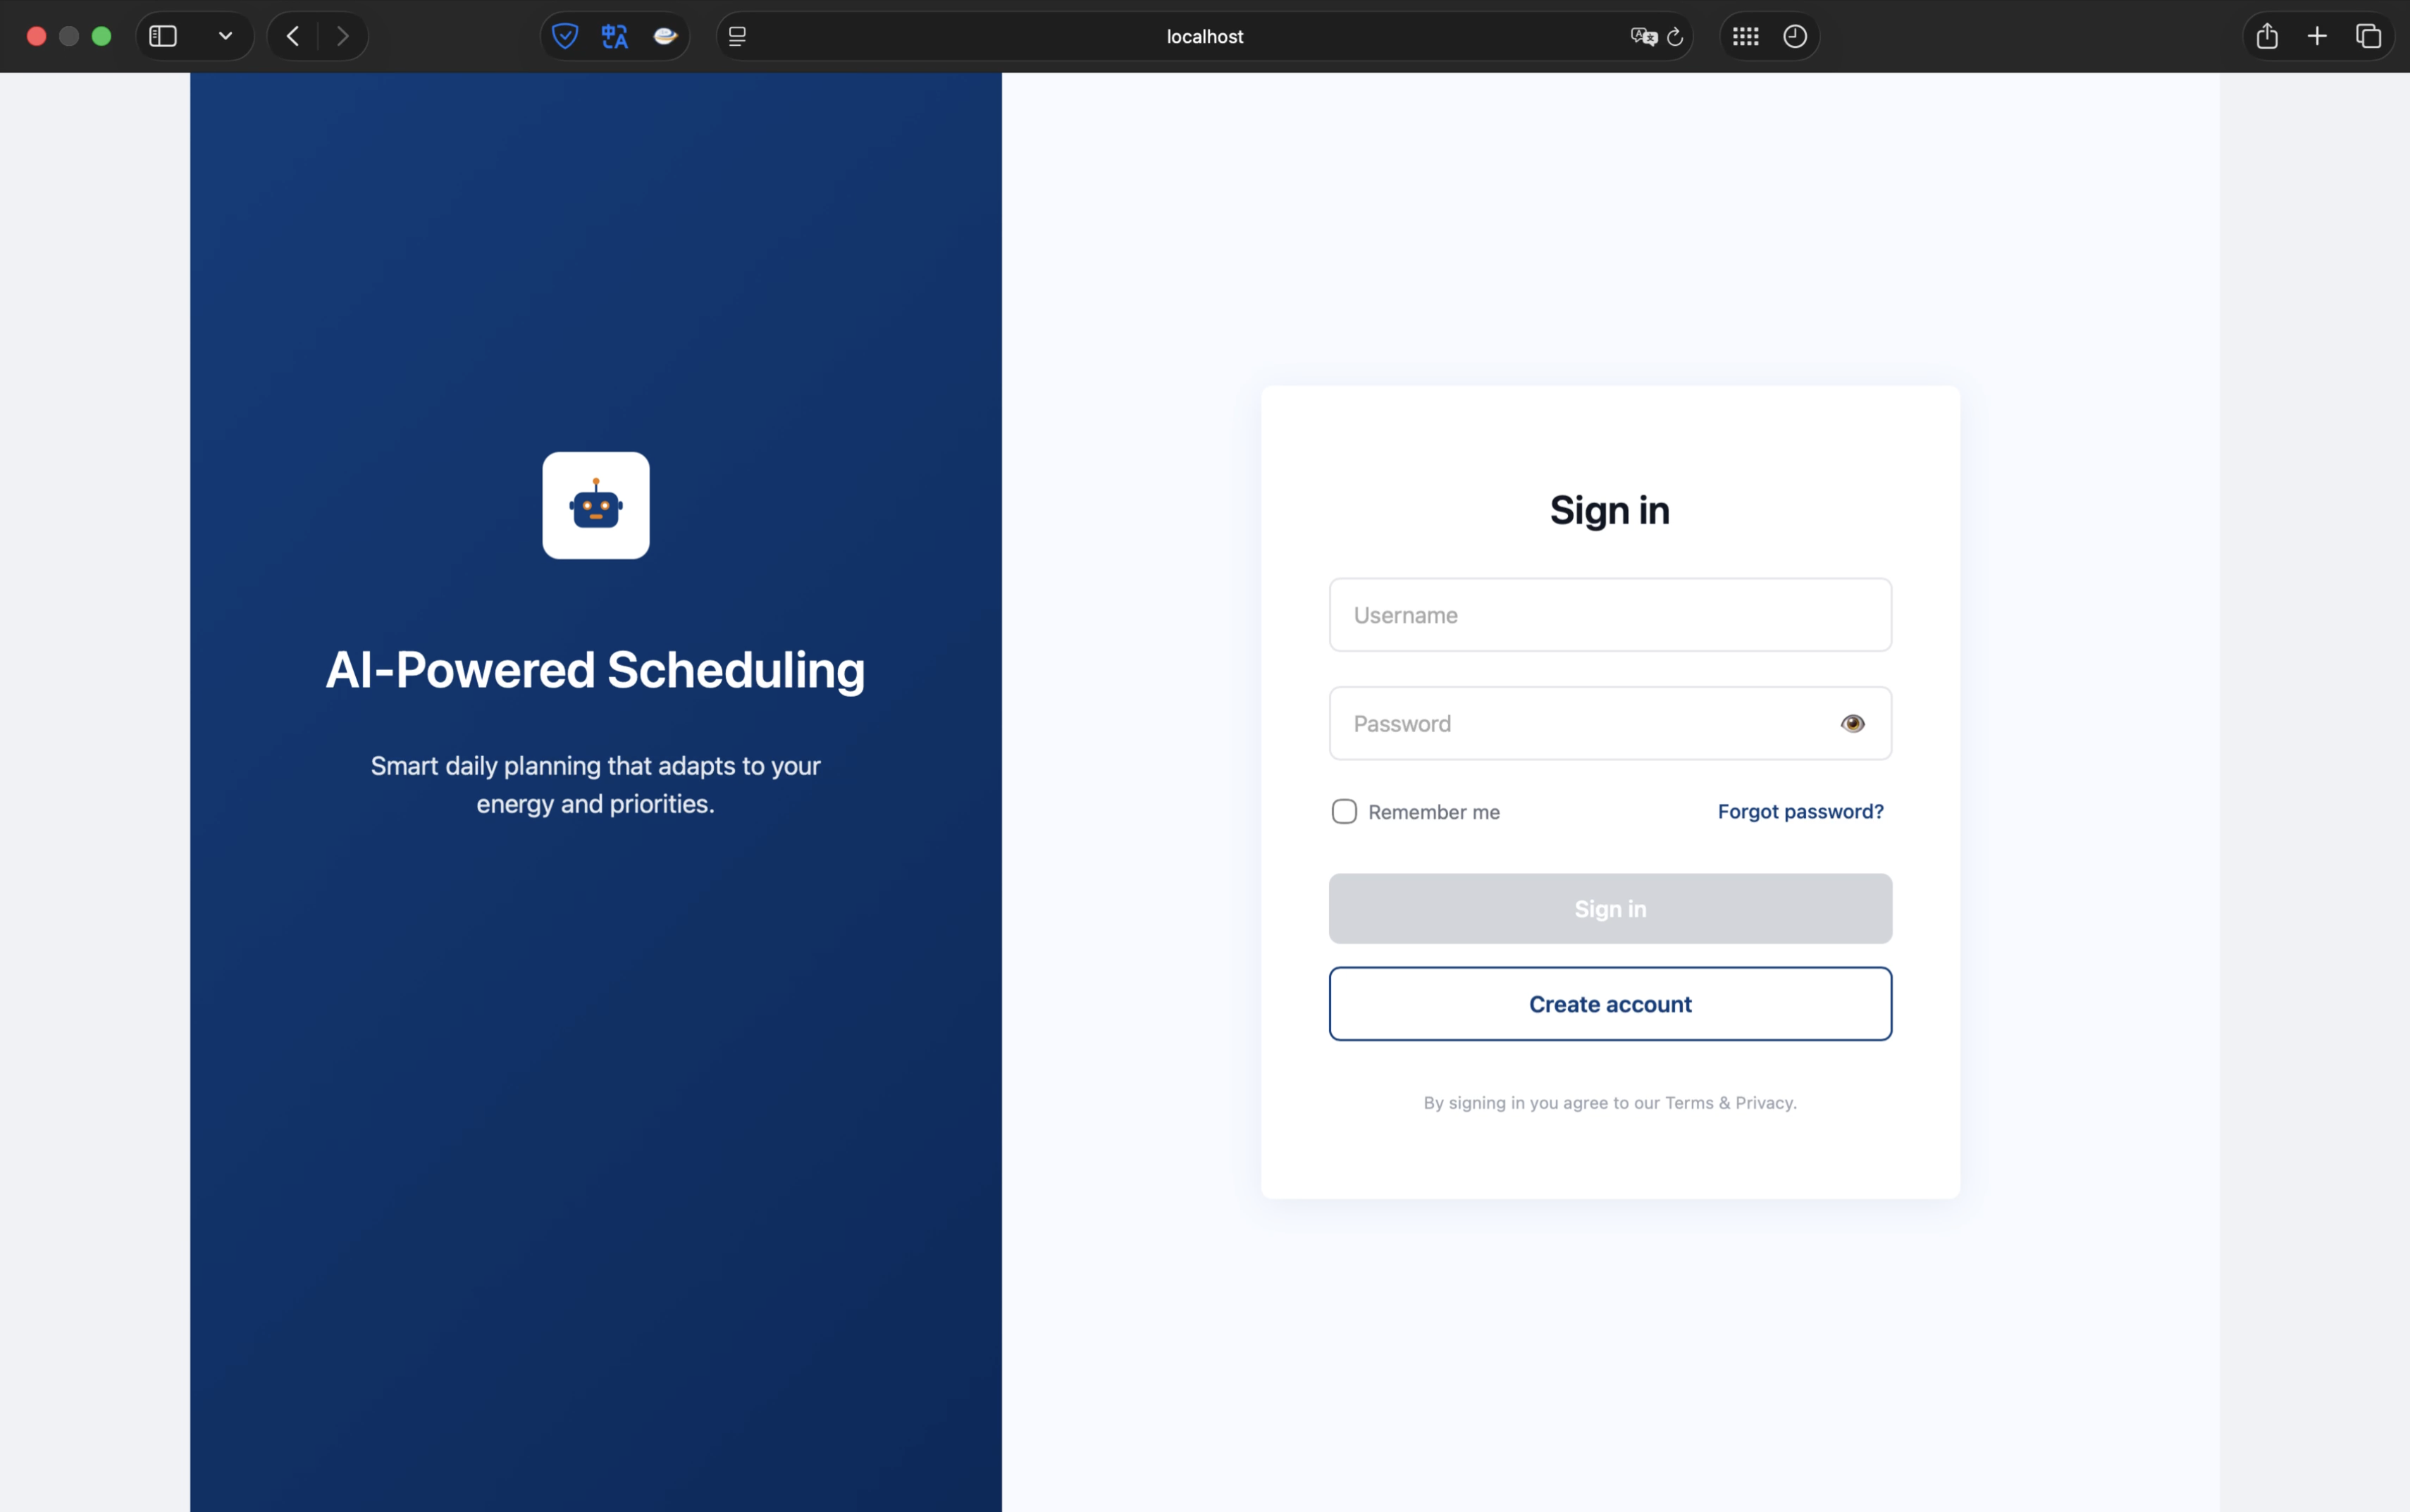
\includegraphics[height=200pt]{Images/System/cover.png}
        \caption{AI-Powered Scheduling System}
        \label{system_cover}
    \end{figure}



%-----------------------
% Problem Description
%-----------------------
\section{Problem Description}

    Effective time management is a persistent challenge in the modern era, where individuals are increasingly burdened by overlapping professional, academic, and personal demands. Traditional task management tools—such as calendars and to-do lists—provide static interfaces that rely heavily on user discipline and manual updates. They lack contextual awareness and cannot adapt dynamically to changes in user workload, energy, or motivation. This often leads to inefficiency, missed deadlines, and heightened stress.
    
    The problem lies in the absence of intelligent reasoning and adaptive personalization in existing scheduling tools. Most applications fail to interpret a user’s behavioral patterns or optimize task order based on fluctuating mental and physical states. Furthermore, users frequently experience decision paralysis—a state in which they have available time but cannot decide what to prioritize—resulting in unproductive downtime.
    
    To address these limitations, this project introduces an AI-Powered scheduling system that leverages data-driven task evaluation and reasoning-based scheduling. The system learns from user history—including completion rates, fatigue patterns, and time usage—to produce personalized daily plans. By balancing workload and recovery periods, it supports sustainable productivity and mental well-being.
    
    From a broader perspective, the system contributes to ongoing research in human-centered artificial intelligence and intelligent decision-making systems. It exemplifies how computational reasoning can enhance everyday productivity tools, making them more adaptive, context-aware, and aligned with human cognitive and emotional needs.



%-----------------------
% Solutions
%-----------------------
\section{Solutions}

    Our \textbf{AI-Powered Scheduling System} is designed to provide personalized, adaptive, and intelligent time management. It integrates artificial intelligence reasoning and user-centered design to help individuals plan tasks efficiently while maintaining well-being.
    
    The system is composed of two major parts: 
    
    \begin{enumerate}
        \item \textbf{Front-End Interface}
            \begin{itemize}
                \item Features an intuitive weekly timetable and task board for visualizing, adding, and editing both fixed and flexible tasks through an interactive calendar view.
                \item Integrates an AI chatbot that understands natural language commands, enabling users to create, update, or delete tasks conversationally.
                \item Supports real-time feedback, task-status transitions, and adaptive rescheduling through intelligent scheduler execution.
                \item Provides analytical dashboards (daily and weekly reports) with dynamic charts that visualize productivity, energy, and stress trends.
            \end{itemize}
        
        \item \textbf{Back-End Intelligence} \\
            The back-end intelligence comprises two key reasoning modules:
            \begin{itemize}
                \item \textbf{Task Evaluation Model} – a neural network that predicts each task’s energy cost and pressure level based on user data and task history. It introduces a Historical Impact Weight (HIW) mechanism to model how past tasks influence current performance.
                \item \textbf{Scheduler} – a rule-based engine that arranges tasks into a feasible timetable by prioritizing deadlines and user-defined importance. It ensures workload balance and automatically allocates rest periods to prevent fatigue.
            \end{itemize}
    \end{enumerate}
    
    The system achieves several functions: 
    
    \begin{enumerate}
        \item \textbf{Intelligent Task Ranking}: Tasks are evaluated and ranked according to urgency, priority, and predicted energy/pressure levels.
        \item \textbf{Adaptive Scheduling}: Automatically assigns tasks to optimal time slots, considering fixed appointments and dynamic updates.
        \item \textbf{Rest Time Optimization}: Determines ideal rest intervals using an evolutionary algorithm to enhance recovery and long-term efficiency.
        \item \textbf{Natural Language Interaction}: (Optional LLM integration) Users can describe tasks in plain language, and the system extracts relevant parameters (e.g., deadline, duration).
        \item \textbf{Personalized Learning}: The system refines its scheduling strategy based on user feedback and past behavior patterns.
    \end{enumerate}
    
    \subsection{Task Evaluation Model}
    
        The \textbf{Task Evaluation Model} serves as the system’s predictive intelligence component. Its primary objective is to estimate how each task influences a user’s energy consumption and mental pressure, thereby enabling intelligent scheduling and ranking based on predicted physical and cognitive load.
    
        The model takes as input structured task attributes—such as type, duration, and difficulty—and outputs two key indicators:
    
        \begin{center}
            $(\Delta E, \Delta P) = f(\text{type}, \text{duration}, \text{difficulty})$
        \end{center}
    
        where $\Delta E$ denotes the predicted change in energy (energy loss), and $\Delta P$ represents the predicted change in psychological pressure (pressure increase).
    
        \subsubsection{Data Preparation}
    
            To train the predictive model, two primary datasets are used:
    
            \begin{itemize}
                \item \textbf{stats\_check.csv} — continuous biometric logs collected throughout the day, recording each user’s \textbf{Energy} and \textbf{Pressure} levels at specific timestamps.
                \item \textbf{schedule.csv} — task logs detailing each activity’s user, task type, start/end time, and difficulty rating.
            \end{itemize}
    
            A dedicated preprocessing script (\textbf{data\_preprocessing.py}) combines these two sources through time-aligned interpolation. For each task instance, the system:
    
            \begin{enumerate}
                \item Locates the user’s Energy and Pressure data on the same date.
                \item Interpolates the values at both the task’s start and end timestamps.
                \item Computes the deltas:
                        
                    \begin{center}
                        $\Delta E = E_{end} - E_{start}, \quad \Delta P = P_{end} - P_{start}$
                    \end{center}
            
                    These deltas represent the physical and cognitive effects associated with performing the task.  
                    The preprocessing procedure robustly handles edge cases such as:
                    
                    \begin{itemize}
                        \item Missing or incomplete biometric records,
                        \item Single-point or sparse daily logs,
                        \item Cross-midnight or invalid time ranges.
                    \end{itemize}
            \end{enumerate}
    
            The resulting dataset (\textbf{new\_tasks\_df.csv}) forms a structured learning table, where each task is paired with its observed energy and pressure variations.
    
        \subsubsection{Feature Engineering}
    
            Before model training, several features are extracted and numerically encoded:
    
            \begin{center}
                \begin{tabular}{l l l}
                    \toprule
                    \textbf{Feature} & \textbf{Description} & \textbf{Type} \\ \midrule   
                    Task type & Encoded categorical label (via LabelEncoder) & Categorical (int) \\
                    Difficulty & User-defined perceived difficulty (0–5 scale) & Numeric \\
                    Duration & Computed task duration (in minutes) & Numeric \\ \bottomrule
                \end{tabular}
            \end{center}
    
            Additional derived labels include:
            \begin{itemize}
                \item \textbf{energy\_loss}: difference in Energy between task end and start,
                \item \textbf{pressure\_increase}: difference in Pressure between task end and start.
            \end{itemize}
    
        \subsubsection{Model Training and Evaluation}
    
            Two independent regression models are trained to predict Energy Loss and Pressure Increase respectively. Both use the same input features [\textbf{type}, \textbf{difficulty}, \textbf{duration}].

            \begin{enumerate}
                \item \textbf{Model Choice}

                    A \textbf{Random Forest Regressor} is adopted for both targets due to its robustness to noise and missing data, nonlinear feature interaction handling, and interpretability through feature importance analysis.

                \item \textbf{Training Process}

                    \begin{enumerate}
                        \item The dataset is split 80/20 into training and test sets.
                        \item Separate models are trained for each target:
                        
                            \begin{center}
                                $f_E(x) \rightarrow \widehat{\Delta E}, \quad f_P(x) \rightarrow \widehat{\Delta P}$
                            \end{center}
                        
                        \item Model performance is evaluated using:
                        
                            \begin{itemize}
                                \item MAE (Mean Absolute Error)
                                \item MSE (Mean Squared Error)
                                \item $R^2$ Score (Goodness of fit)
                            \end{itemize}
                    \end{enumerate}

                \item \textbf{Evaluation Output}

                    === Energy Loss Prediction === \\
                    MAE: 0.6154976455054124 \\
                    MSE: 0.7161091879304533 \\
                    R²: 0.05477522739025942 
            
                    === Pressure Increase Prediction === \\
                    MAE: 0.6326830109599901 \\
                    MSE: 0.7067960090389993 \\
                    R²: -0.13040842378934858 \\
                    
            \end{enumerate}
    
            Both models are then persisted as serialized \textbf{.pkl} files using \textbf{joblib}: 
            
            \begin{itemize}
                \item \textbf{energy\_loss\_model.pkl}
                \item \textbf{pressure\_increase\_model.pkl}
                \item \textbf{task\_label\_encoder.pkl}
            \end{itemize}
    
        \subsubsection{Task Scoring and Application}
    
            Once trained, the model is applied to new or upcoming tasks (from \textbf{new\_tasks\_df.csv}) to predict:
    
            \begin{center}
                $\text{Predicted Load} = \{\widehat{\Delta E}, \widehat{\Delta P}\}$
            \end{center}
    
            These predicted values are subsequently integrated into the Scheduler and Task Ranking modules to:
    
            \begin{itemize}
                \item Prioritize low-fatigue time slots for high-energy tasks,
                \item Avoid consecutive high-pressure activities,
                \item Recommend rest intervals when cumulative predicted load exceeds a threshold.
            \end{itemize}
    
            Through this integration, the system achieves both predictive awareness and adaptive scheduling, ensuring an optimal balance between productivity and user well-being.
    
    \subsection{Scheduler}
    
        The \textbf{Scheduler} is the central reasoning engine of the AI-powered Scheduling System. Its main objective is to transform a collection of user tasks—both fixed and flexible—into a feasible, adaptive, and optimized timetable that balances productivity with well-being. It embodies the system’s intelligent reasoning capability, enabling real-time adaptation to user behavior, task constraints, and time availability. 
        
        The design of the Scheduler integrates \textbf{rule-based logic}, \textbf{heuristic optimization}, and \textbf{data-driven evaluation}. It not only arranges tasks efficiently but also ensures the user receives adequate rest, minimizing cognitive fatigue and maintaining consistent performance throughout the day. The workflow of the scheduler is shown in Figure~\ref{scheduler}. 

        \begin{figure}[H]
            \centering
            \includesvg[width=0.6\textwidth]{Images/System/scheduler.svg}
            \caption{Scheduler Workflow}
            \label{scheduler}
        \end{figure}

        \subsubsection{Core Architecture and Logic}

            \begin{enumerate}
                \item \textbf{Task Categorization}

                    All incoming tasks are divided into two primary types: 

                    \begin{itemize}
                        \item \textbf{Fixed Tasks}: Events that have immutable start and end times (e.g., meetings, classes).
                        \item \textbf{Flexible Tasks}: Tasks with adjustable time windows that the system can optimize (e.g., studying, project work).
                    \end{itemize}

                    This distinction allows the Scheduler to maintain temporal integrity (fixed commitments first) while using flexible intervals to adaptively optimize user time.

                \item \textbf{Scheduling Pipeline}

                    The Scheduler operates through a structured multi-stage process:

                    \begin{itemize}
                        \item \textbf{Initialization}: All fixed tasks are inserted into the timeline in chronological order. The system identifies available windows between fixed tasks. 
                        \item \textbf{Task Sorting}: Flexible tasks are sorted by earliest deadline, priority, and expected duration. This ensures time-critical and high-importance tasks are handled first.
                        \item \textbf{Progressive Fitting}: For each flexible task, the Scheduler traverses available windows sequentially. It checks three constraints: \textbf{1.} The task cannot be scheduled before the current time. \textbf{2.} It must finish before its deadline. \textbf{3.} It must not exceed the available duration window (with a 25\% buffer margin to absorb unexpected changes). Tasks violating any constraint are skipped or reported as unscheduled.
                        \item \textbf{Conflict Handling and Reallocation}: If inserting a new fixed task disrupts existing ones, the Scheduler automatically extracts affected tasks, rebuilds free windows, and reinserts displaced tasks using the same priority-based fitting logic. This guarantees adaptive reorganization without manual intervention.
                    \end{itemize}
            \end{enumerate}

        \subsubsection{Rest Time Distribution}

            To ensure sustainable performance, the Scheduler allocates \textbf{optimal rest intervals} between tasks: 

            \begin{enumerate}
                \item The system uses a \textbf{Sigmoid rest-feedback function} to model the diminishing returns of rest time (i.e., a short rest boosts performance sharply, but excessive rest yields less benefit).
                
                \item Using Lagrange multiplier optimization and binary search, the Scheduler distributes the available rest budget among multiple rest slots such that: 

                    \begin{center}
                        $\sum_i r_i (\lambda) = R_{total}$
                    \end{center}
    
                    where $r_i$ represents the rest time allocated to slot i under a global rest-time constraint $R_{total}$.

                \item The method guarantees convergence and fairness among all rest periods, maximizing overall energy recovery and stress reduction.
            \end{enumerate}

            This process mirrors a \textbf{water-filling optimization} approach used in resource allocation problems.

        \subsubsection{Historical Impact Integration}

            To make scheduling context-aware, the Scheduler considers the historical influence of previous tasks:

            \begin{enumerate}
                \item It computes \textbf{task similarity} based on attribute vectors (type, difficulty, duration, etc.) using \textbf{cosine similarity}.
                \item The \textbf{Historical Impact Weight (HIW)} mechanism then adjusts the predicted energy and pressure of a task based on residual fatigue from similar prior tasks:

                \begin{center}
                    $\text{Adjusted\ Energy}_t = E_t + \text{Similarity} \times E_{t-1}$
                \end{center}
            \end{enumerate}

            This approach ensures that performing several similar tasks consecutively increases cumulative fatigue, encouraging more balanced task sequences.

        
        \subsubsection{Computational Efficiency}

            \begin{enumerate}
                \item Task Sorting: $O(N \log N)$
                \item Task Placement: $O(N \times W)$, where W is the number of windows.
                \item Rest Optimization: $O(K \log(1/\epsilon))$, where K is the number of rest slots and $\epsilon$ is the convergence tolerance.
            \end{enumerate}

            Overall, the algorithm achieves practical real-time performance for individual users while maintaining theoretical rigor in optimization.


    \subsection{System Development}
    
        The system development can be divided into three main parts: the \textbf{database construction}, the \textbf{backend development} and \textbf{frontend design}. 

        \subsubsection{Database}

            Our system uses \textbf{MongoDB} as the core database for storing users, tasks, and scheduling information. As a \textbf{NoSQL document database}, MongoDB organizes data in a flexible \textbf{JSON-like structure}, allowing different users’ tasks and records to have dynamic fields such as deadlines, priorities, and predicted energy or stress levels. This flexibility is essential for an adaptive AI scheduling system, where task attributes and user data frequently evolve.
            
            We chose MongoDB because it offers high scalability, schema flexibility, and fast query performance. Its JSON/BSON format integrates seamlessly with our Python-based backend, enabling efficient data exchange between the AI reasoning modules and the web interface. Moreover, MongoDB’s real-time update and indexing features allow the scheduler to react immediately to user input and changes, ensuring smooth, responsive performance even under dynamic workloads.

            For our system, we build a database with three collections: users, fixed-tasks and flexible-tasks. The users collection stores user account information, including fields such as: \{ user\_id, user\_name, password \}. The fixed-tasks collection stores each user's fixed-time task records, with fields: \{ user\_id, task\_name, task\_type, task\_start\_time, task\_end\_time, task\_duration, expected\_difficulty, task\_location, status, created\_at \}. The flexible-tasks collection stores user tasks that can be rescheduled within a flexible time window, in contrast to the strictly timed tasks in fixed-tasks. Compared to fixed-tasks collection, flexible-tasks adds adaptive and predictive attributes (predicted\_energy, predicted\_pressure, task\_priority), but doesn't has explicit start time or end time. 

        \subsubsection{Backend}
        
            The backend of our system is implemented using \textbf{FastAPI}, which provides strong support for data validation, dependency injection, and asynchronous I/O, which makes it particularly well-suited for managing real-time interactions between the user interface and the AI scheduling engine.
            
            The backend architecture follows a modular and service-oriented design, organized into distinct router modules under the \texttt{routers} directory. Each router is responsible for a specific subsystem of the application, ensuring high maintainability, scalability, and clarity in the overall system structure. This modular organization allows independent development and updates to individual modules without affecting the stability of the entire system.
            
            The major router modules are summarized as follows:
            
            \begin{itemize}
                \item \textbf{login.py} – Handles user authentication and session management, including login and credential verification.
                \item \textbf{users.py} – Manages user-related operations such as registration and profile retrieval
                \item \textbf{tasks.py} – Supports CRUD (Create, Read, Update, Delete) operations for both fixed and flexible tasks. It interacts directly with MongoDB to manage user task data efficiently.
                \item \textbf{scheduler.py} – Implements the scheduling logic that determines optimal time slots for flexible tasks based on user availability, task priority, and AI-predicted stress or energy levels.
                \item \textbf{stats\_recording.py} – Collects and records user activity and performance statistics, supporting adaptive learning and system optimization.
                \item \textbf{chatbot.py} – Integrates with the OpenAI API to provide an intelligent conversational interface. Through this module, users can interact with the chatbot.
            \end{itemize}
            
            In addition to the router modules, the backend also includes a \textbf{utils} package containing supporting scripts such as \textbf{scheduler\_updated.py}, which defines the scheduler class.
            
            All API endpoints are defined using FastAPI’s routing system and return data in JSON format to the frontend. The backend manages real-time communication with MongoDB, allowing instant data synchronization when users create, modify, or delete tasks. The combination of FastAPI’s asynchronous processing and MongoDB’s dynamic schema design ensures efficient, low-latency system performance, even under heavy user interaction and concurrent task updates.
            
            Overall, the backend serves as the system’s computational and integration core. It coordinates user input, AI reasoning, and data persistence, forming the foundation of the adaptive and intelligent scheduling experience provided by the platform.
        
        \subsubsection{Frontend (System Presentation)}
        
            \begin{enumerate}
                \item \textbf{Login}
                
                    At the login page, users should type in their username and password, then click the "Sign in" button to login. The system will check if the username and password is correct, if correct, the system will redirect the page to the main timetable, as shown in Figure~\ref{login_correct}, otherwise it will show the problem to the user, as shown in Figure~\ref{login_wrong_username} \& Figure~\ref{login_wrong_password}. 
                    
                    \begin{figure}[H]
                        \centering
                        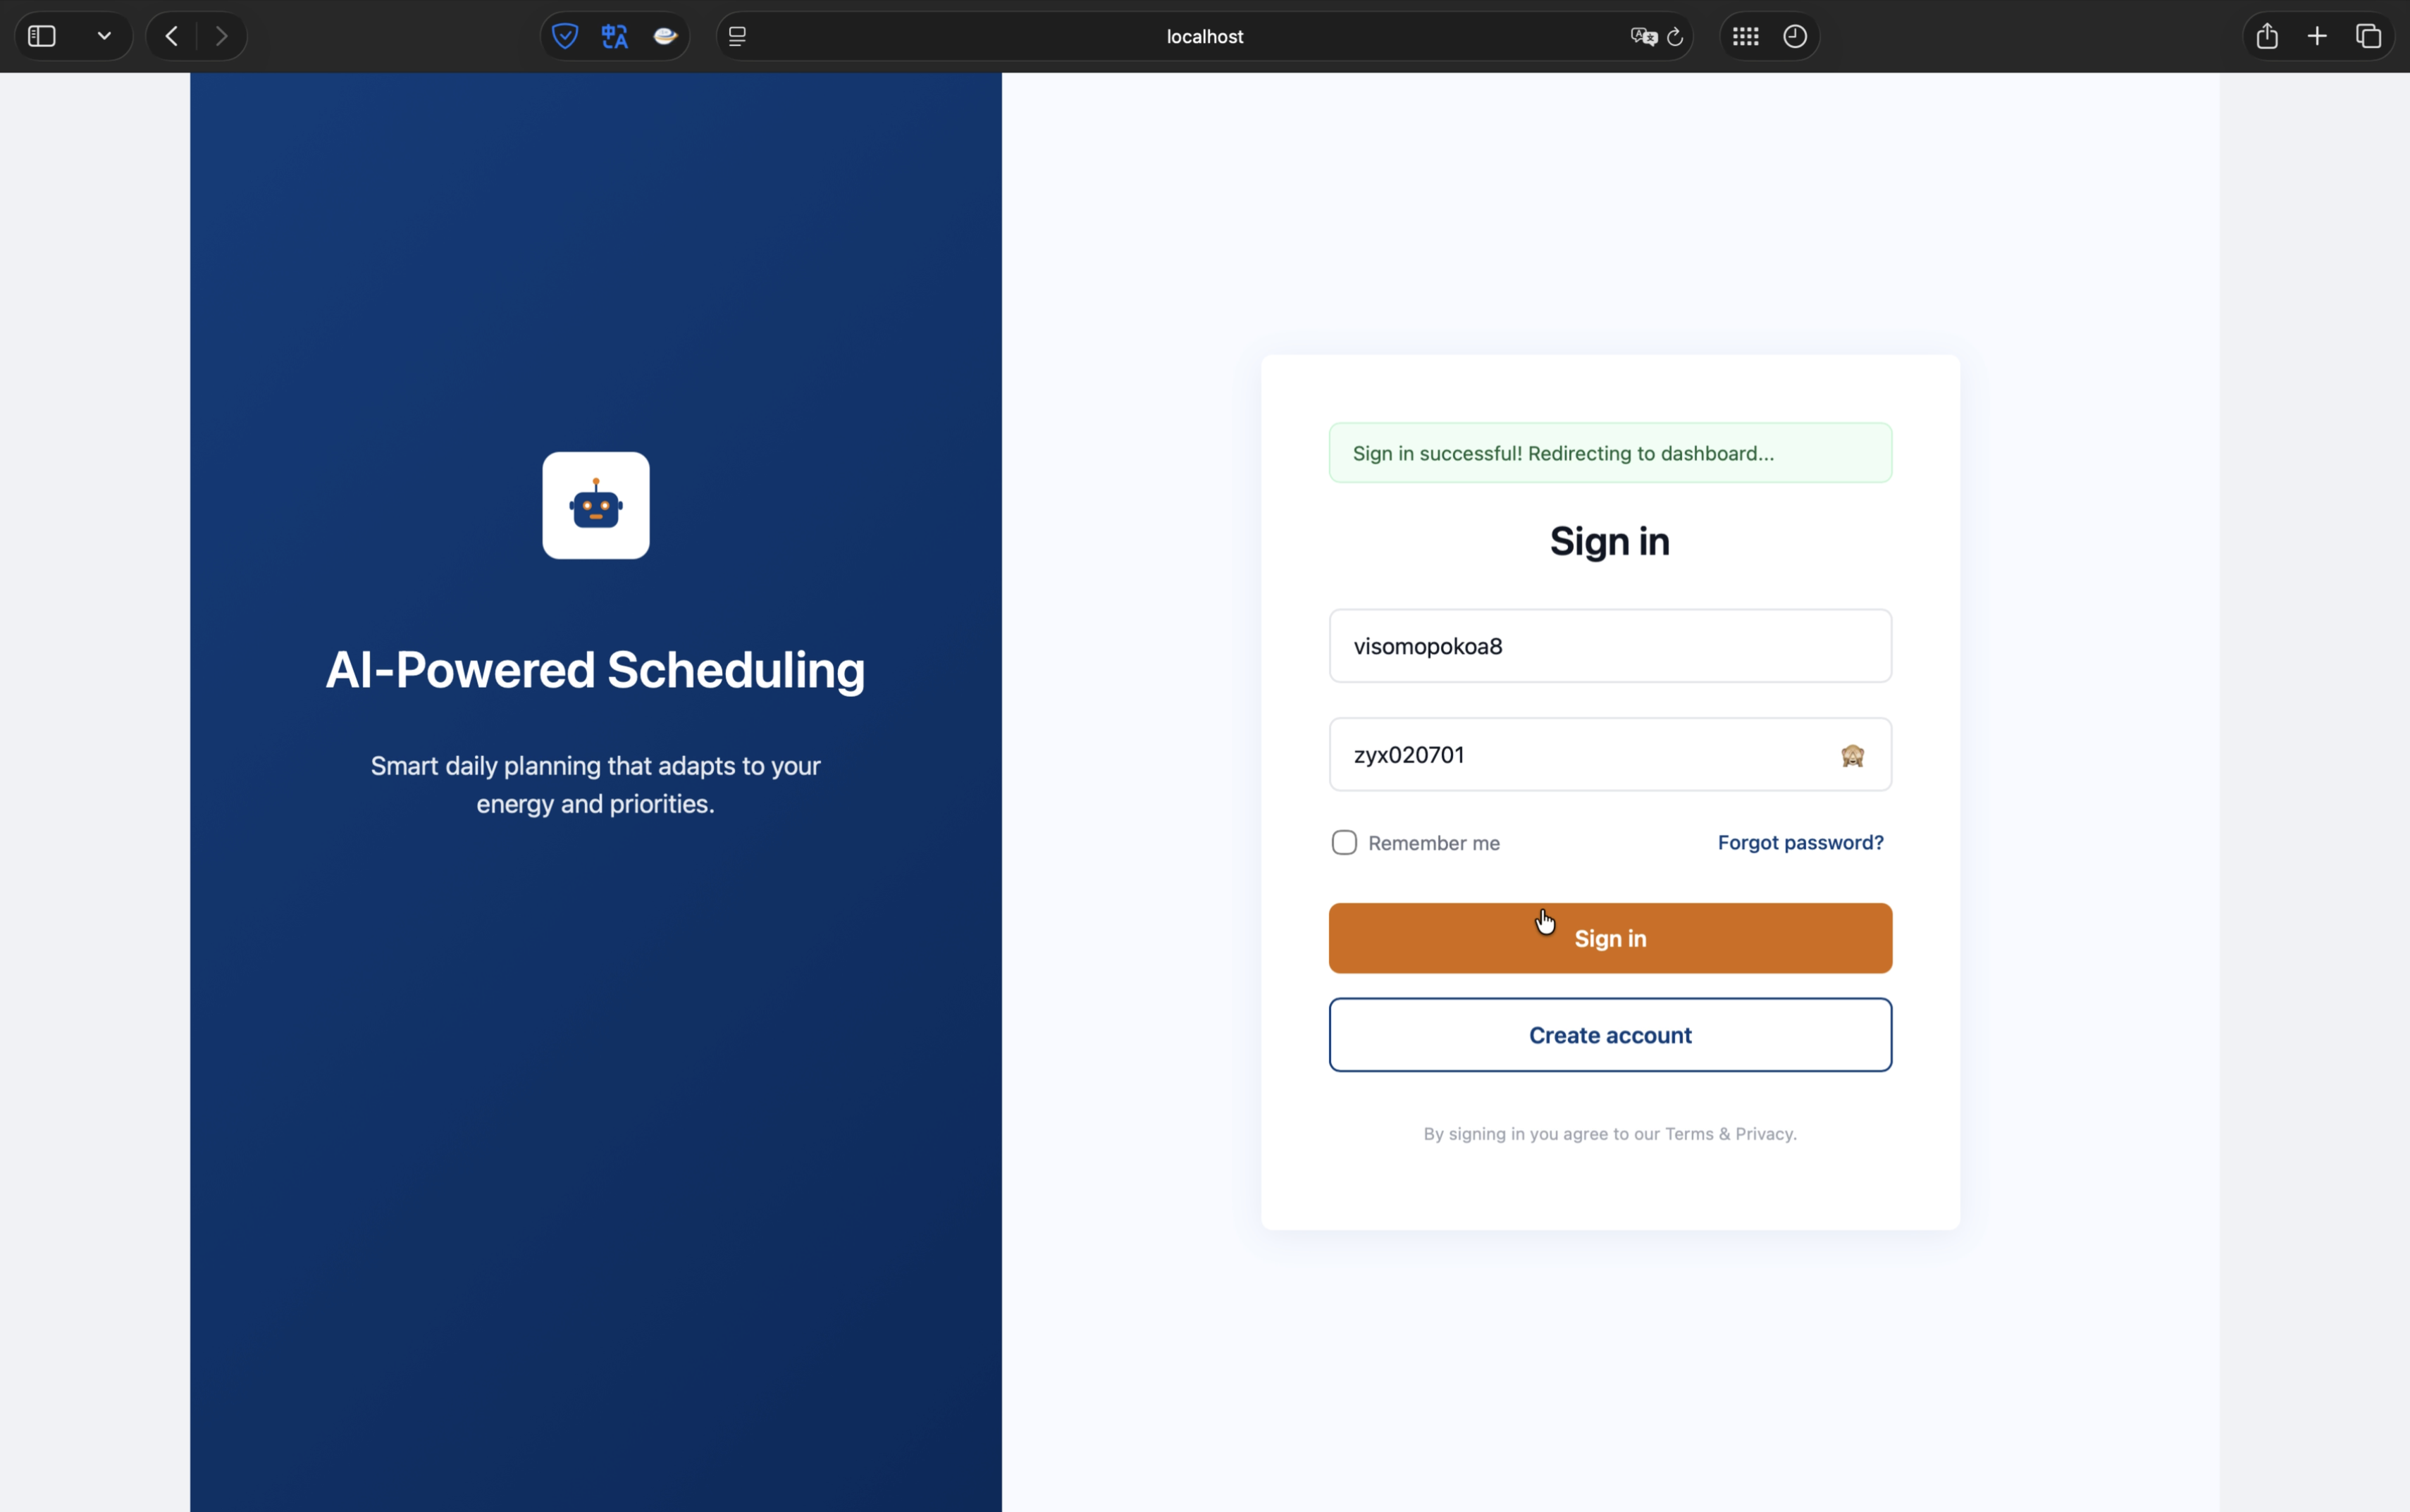
\includegraphics[width=\textwidth]{Images/System/login/redirect.png}
                        \caption{Login Successfully}
                        \label{login_correct}
                    \end{figure}
                    
                    \begin{figure}[H]
                        \begin{minipage}[t]{0.49\textwidth}
                            \centering
                            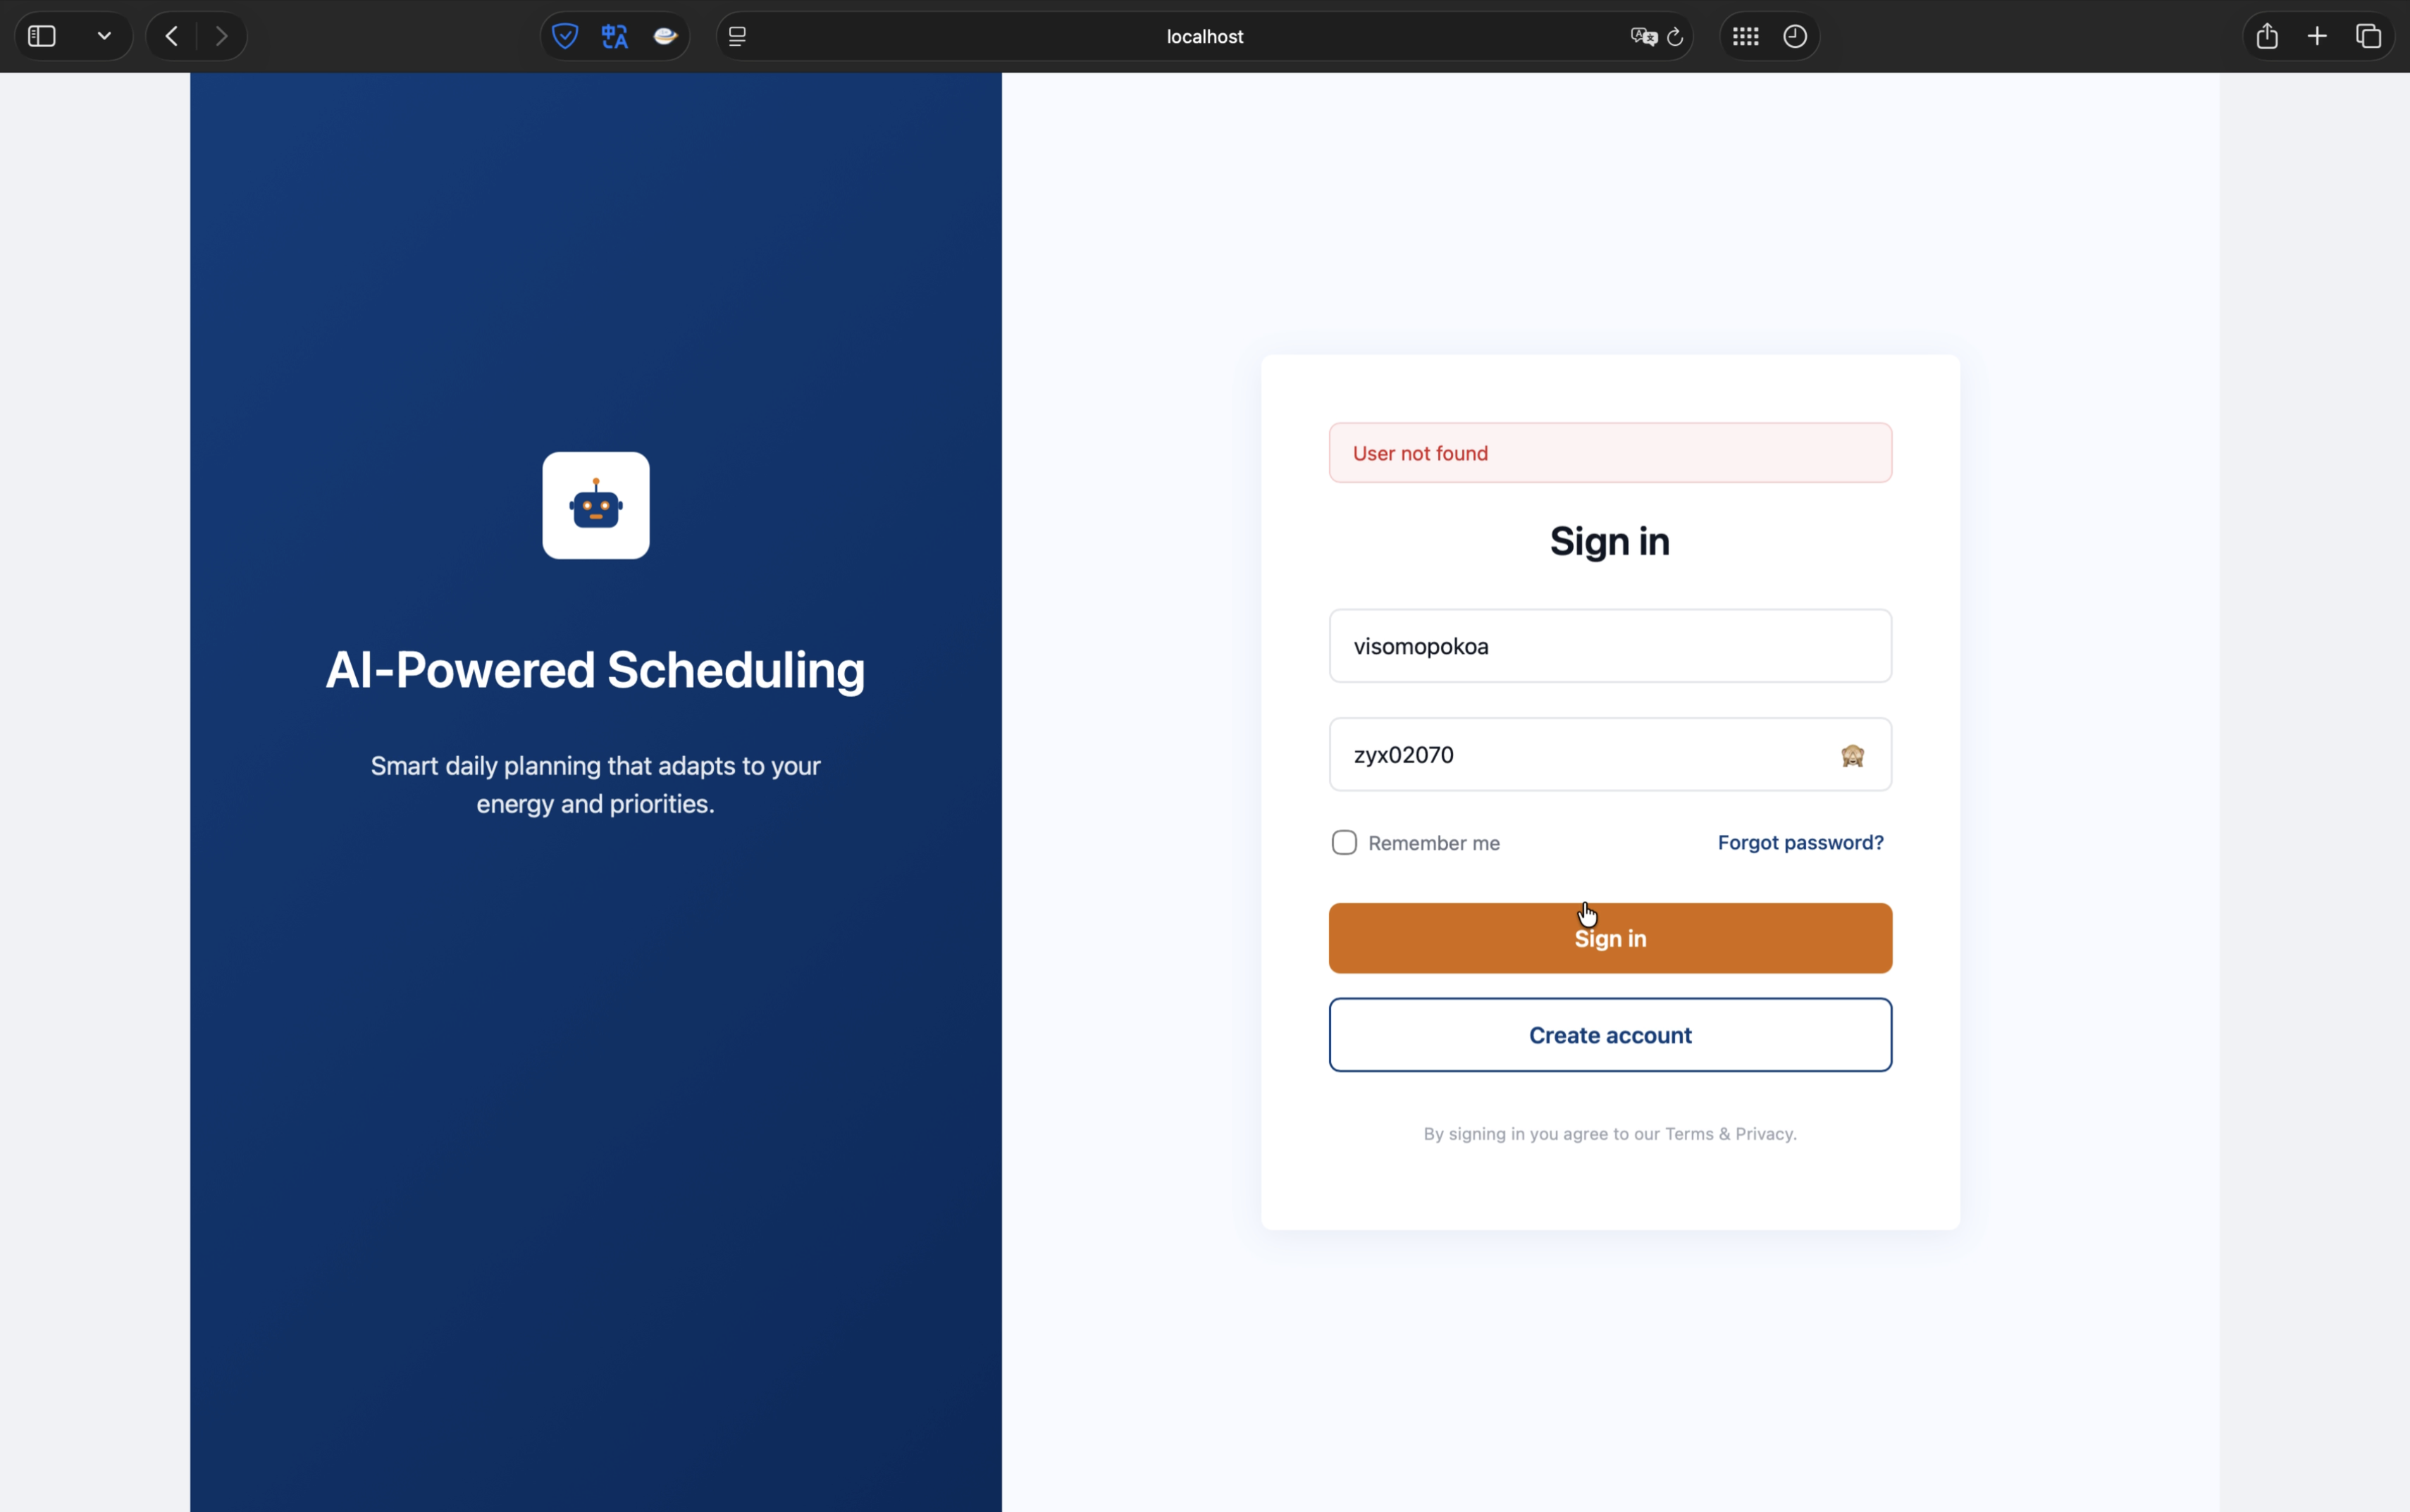
\includegraphics[width=\textwidth]{Images/System/login/username.png}
                            \caption{User Not Found}
                            \label{login_wrong_username}
                        \end{minipage}
                        \hfill
                        \begin{minipage}[t]{0.49\textwidth}
                            \centering
                            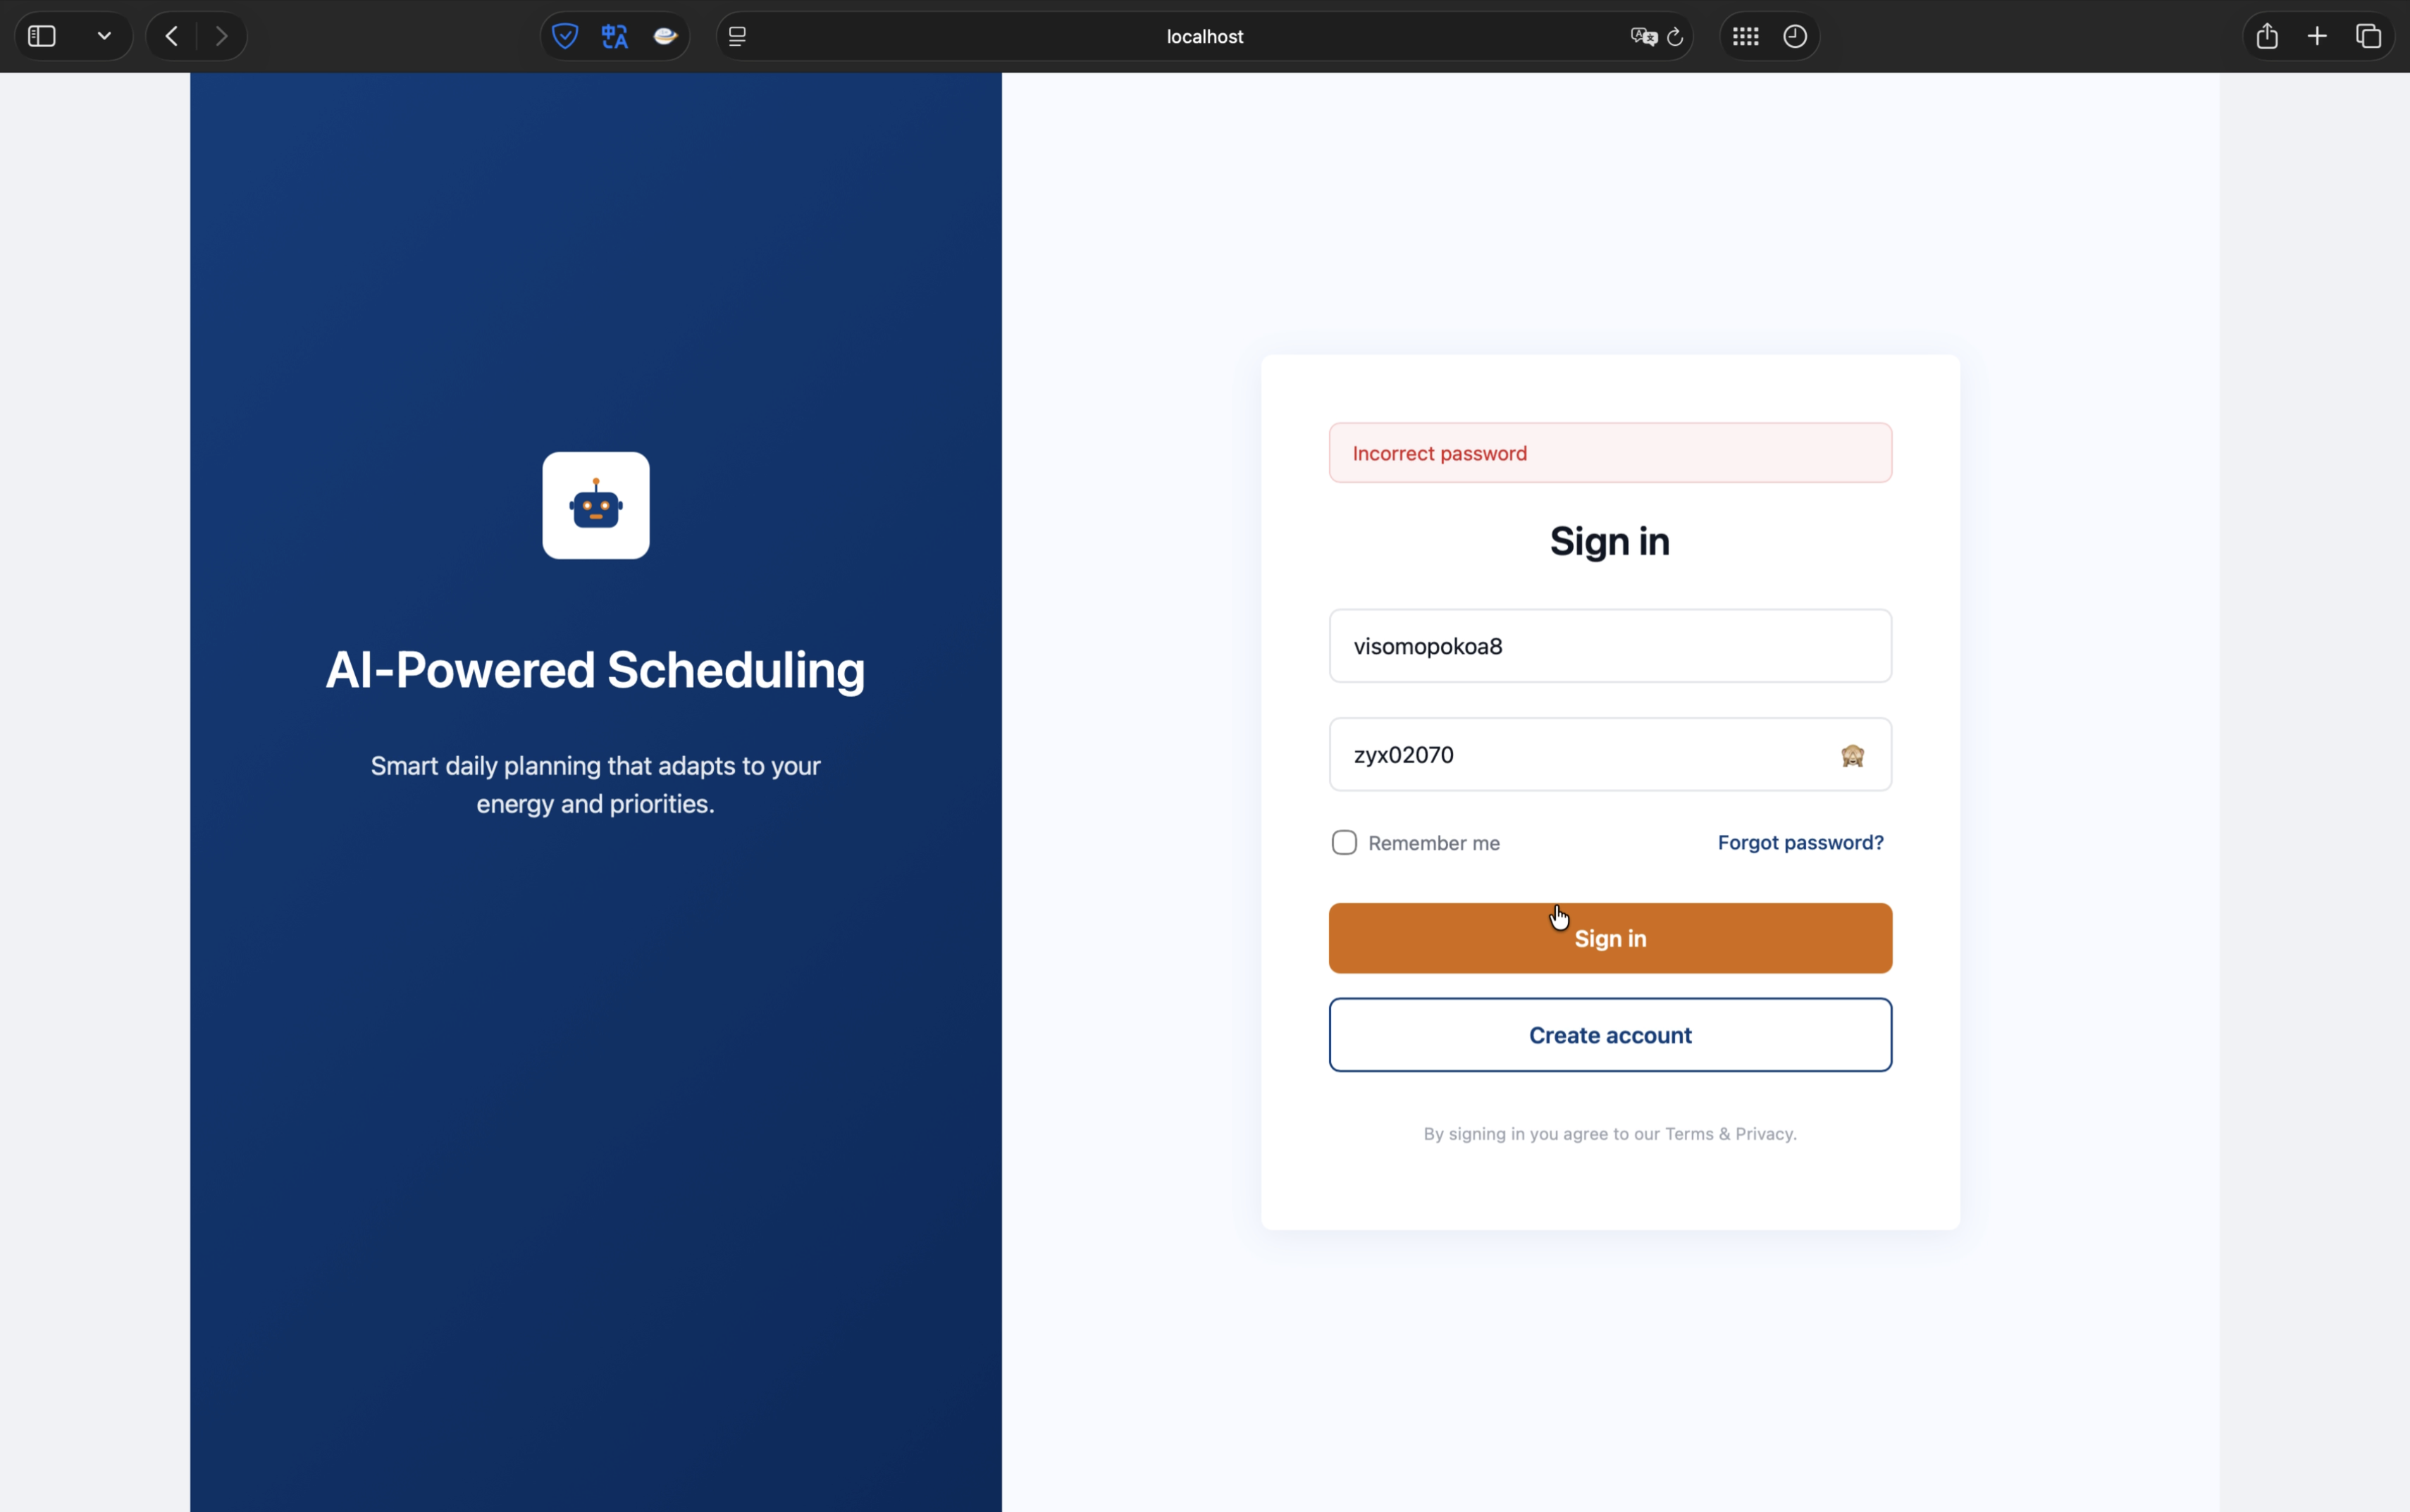
\includegraphics[width=\textwidth]{Images/System/login/password.png}
                            \caption{Incorrect Password}
                            \label{login_wrong_password}
                        \end{minipage}
                    \end{figure}
            
                \item \textbf{Timetable} 

                    After signing in, the first view is the timetable, as Figure~\ref{timetable}, which will list all the registered tasks in it. As show in Figure~\ref{add} to Figure~\ref{aft_delete}, clicking on the white space, the users can add new tasks, clicking on the task block, the users can edit the tasks and even delete them. 

                    \begin{figure}[H]
                        \centering
                        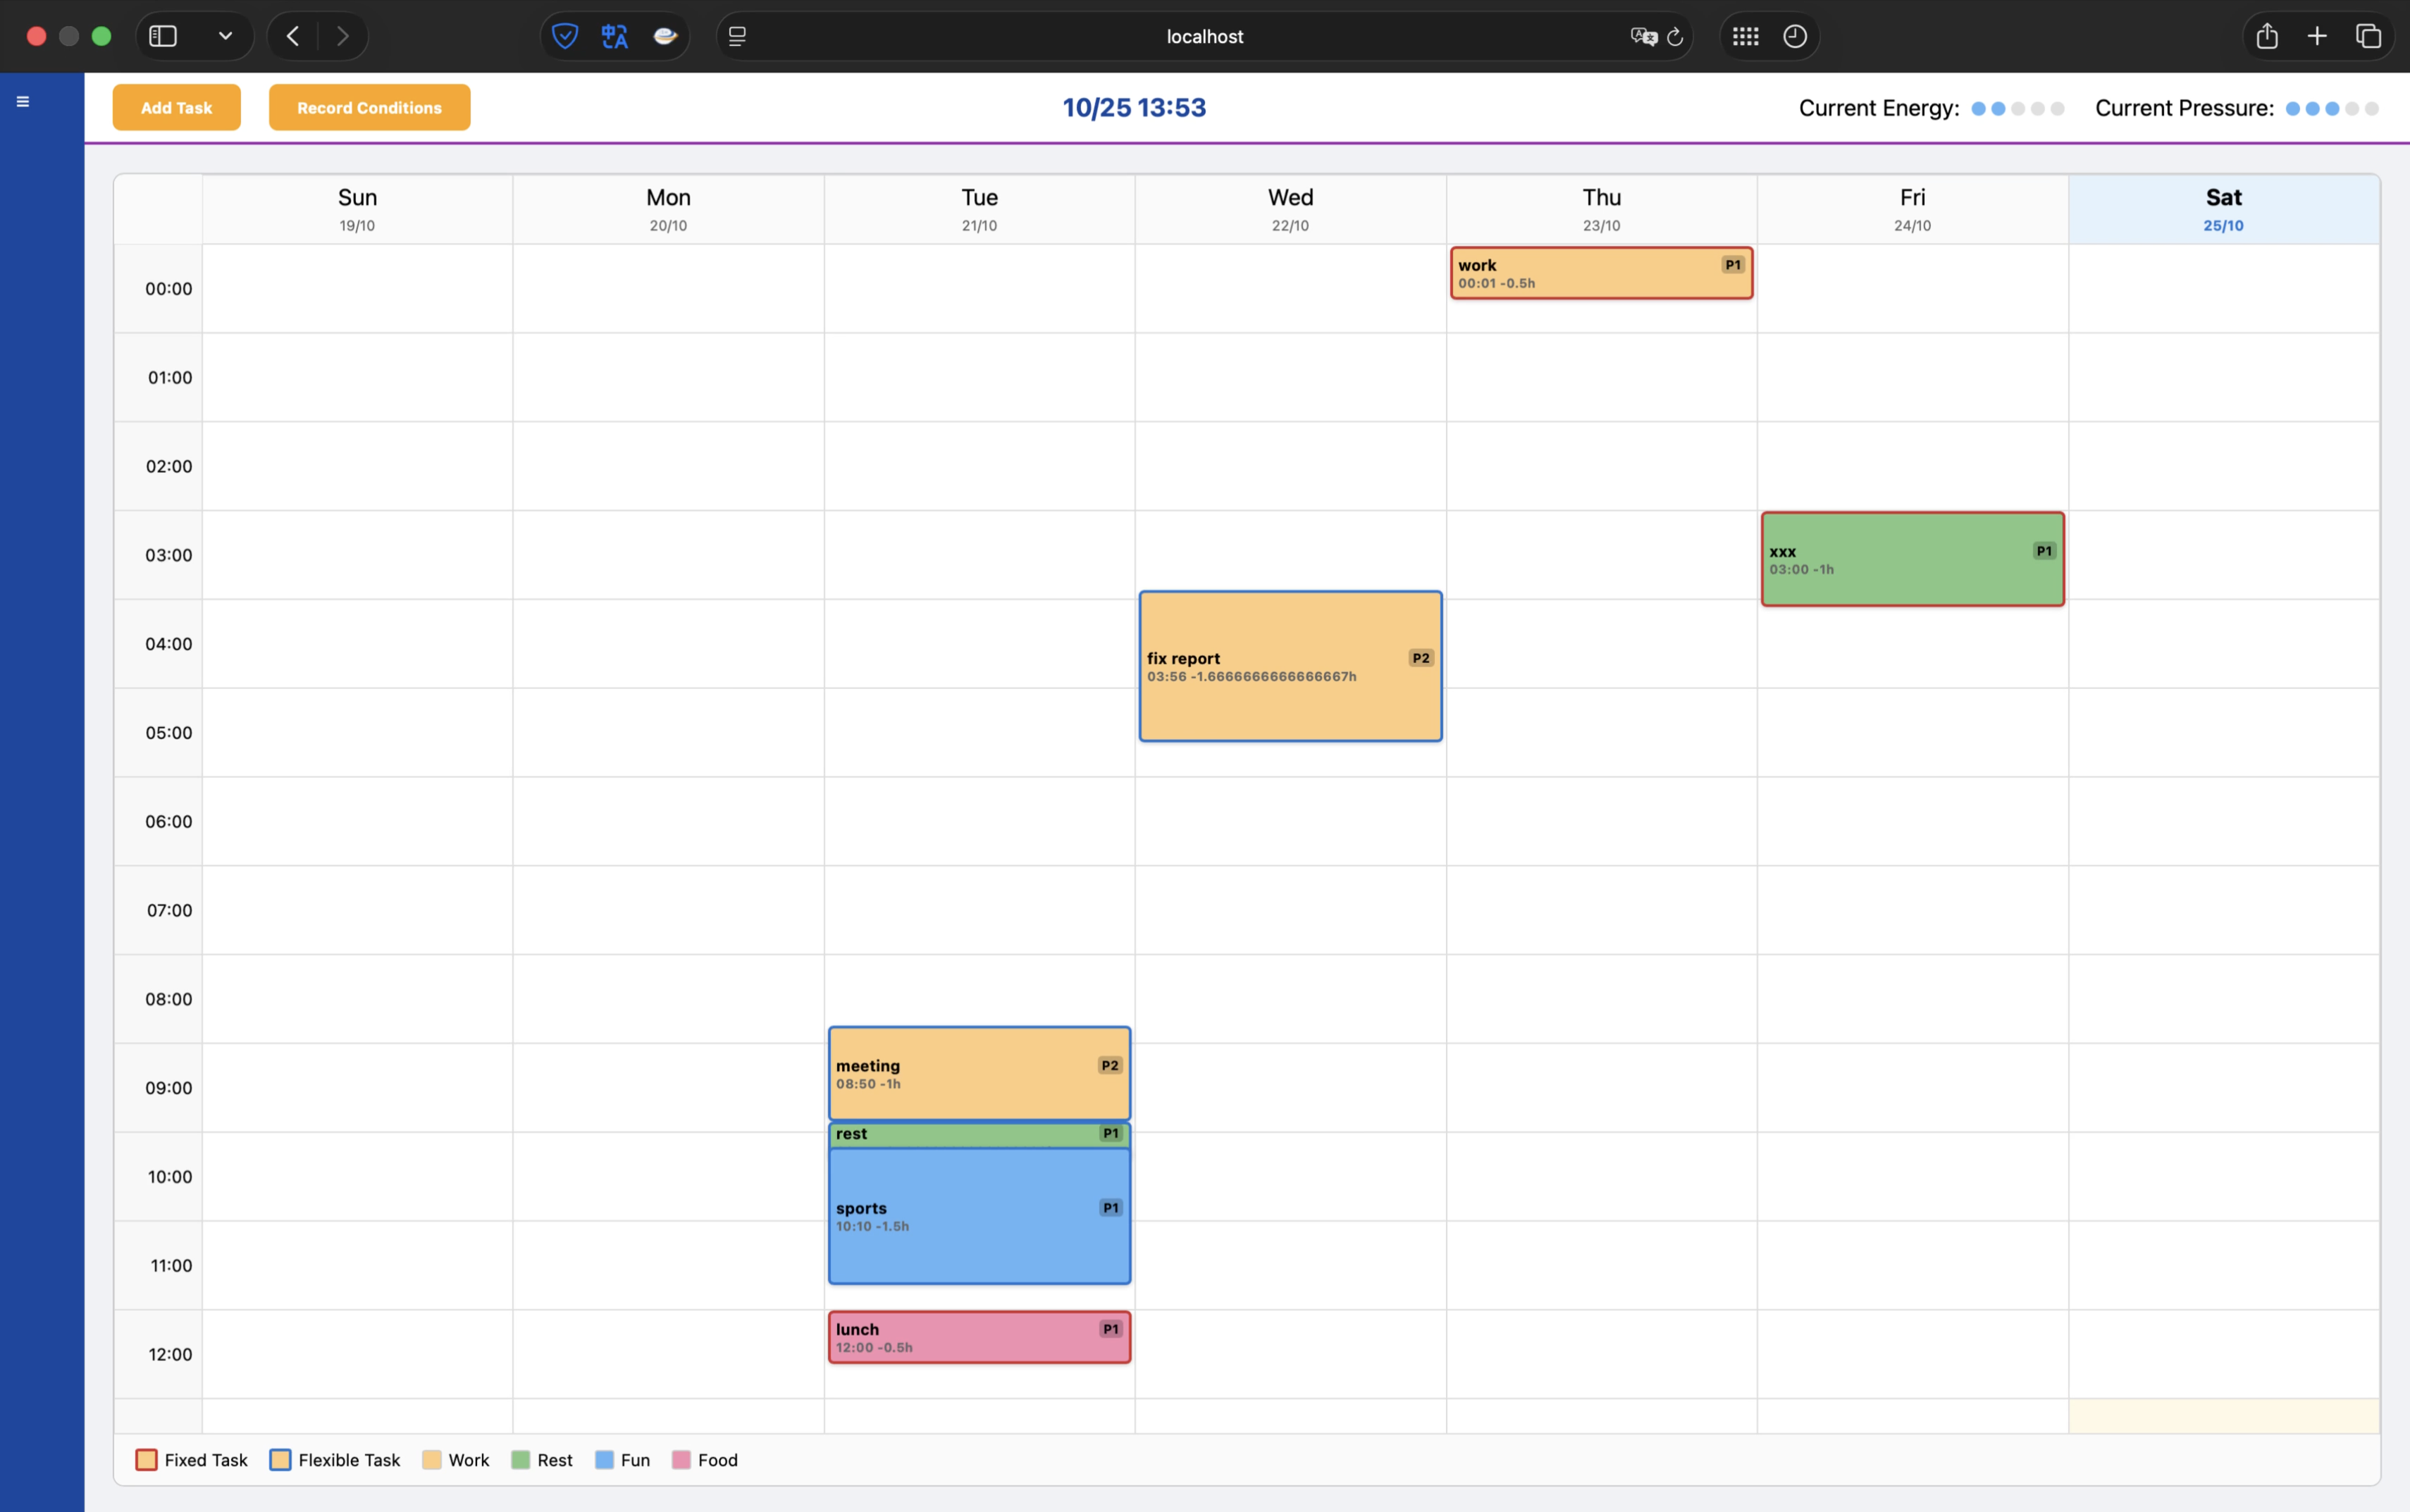
\includegraphics[width=\textwidth]{Images/System/timetable/timetable.png}
                        \caption{Timetable}
                        \label{timetable}
                    \end{figure}

                    \begin{figure}[H]
                        \begin{minipage}[t]{0.49\textwidth}
                            \centering
                            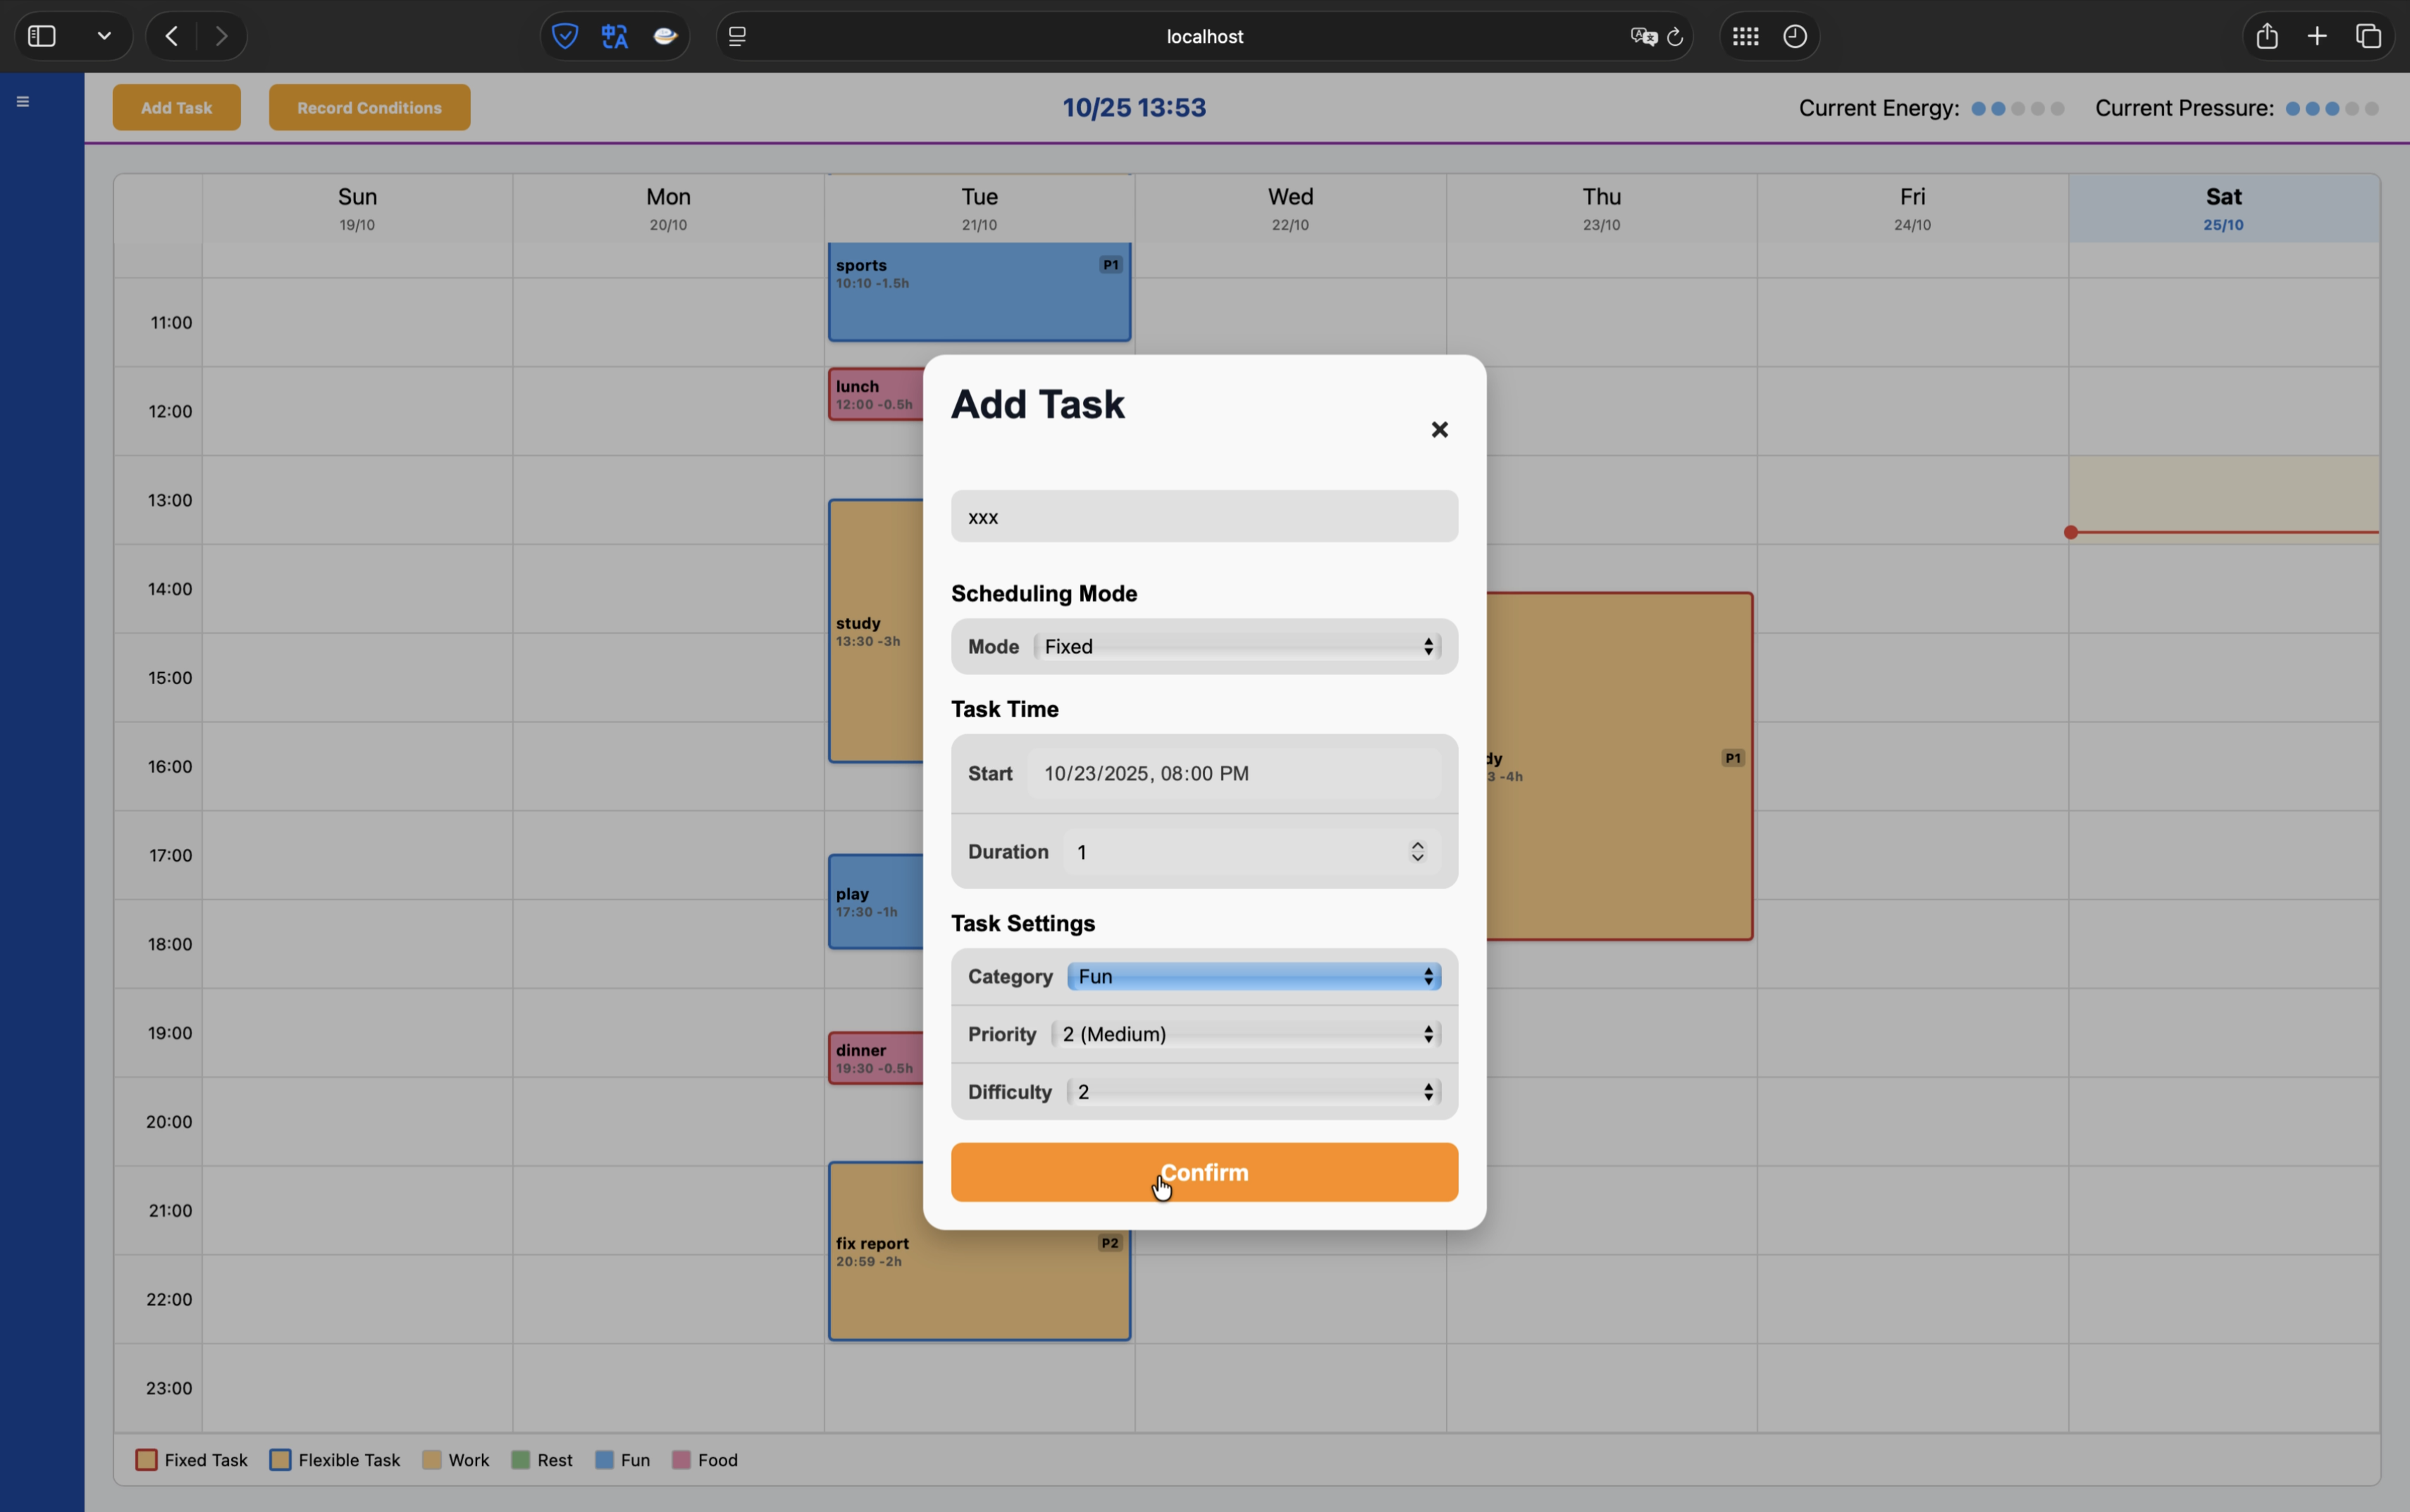
\includegraphics[width=\textwidth]{Images/System/timetable/add.png}
                            \caption{Add Tasks}
                            \label{add}
                        \end{minipage}
                        \hfill
                        \begin{minipage}[t]{0.49\textwidth}
                            \centering
                            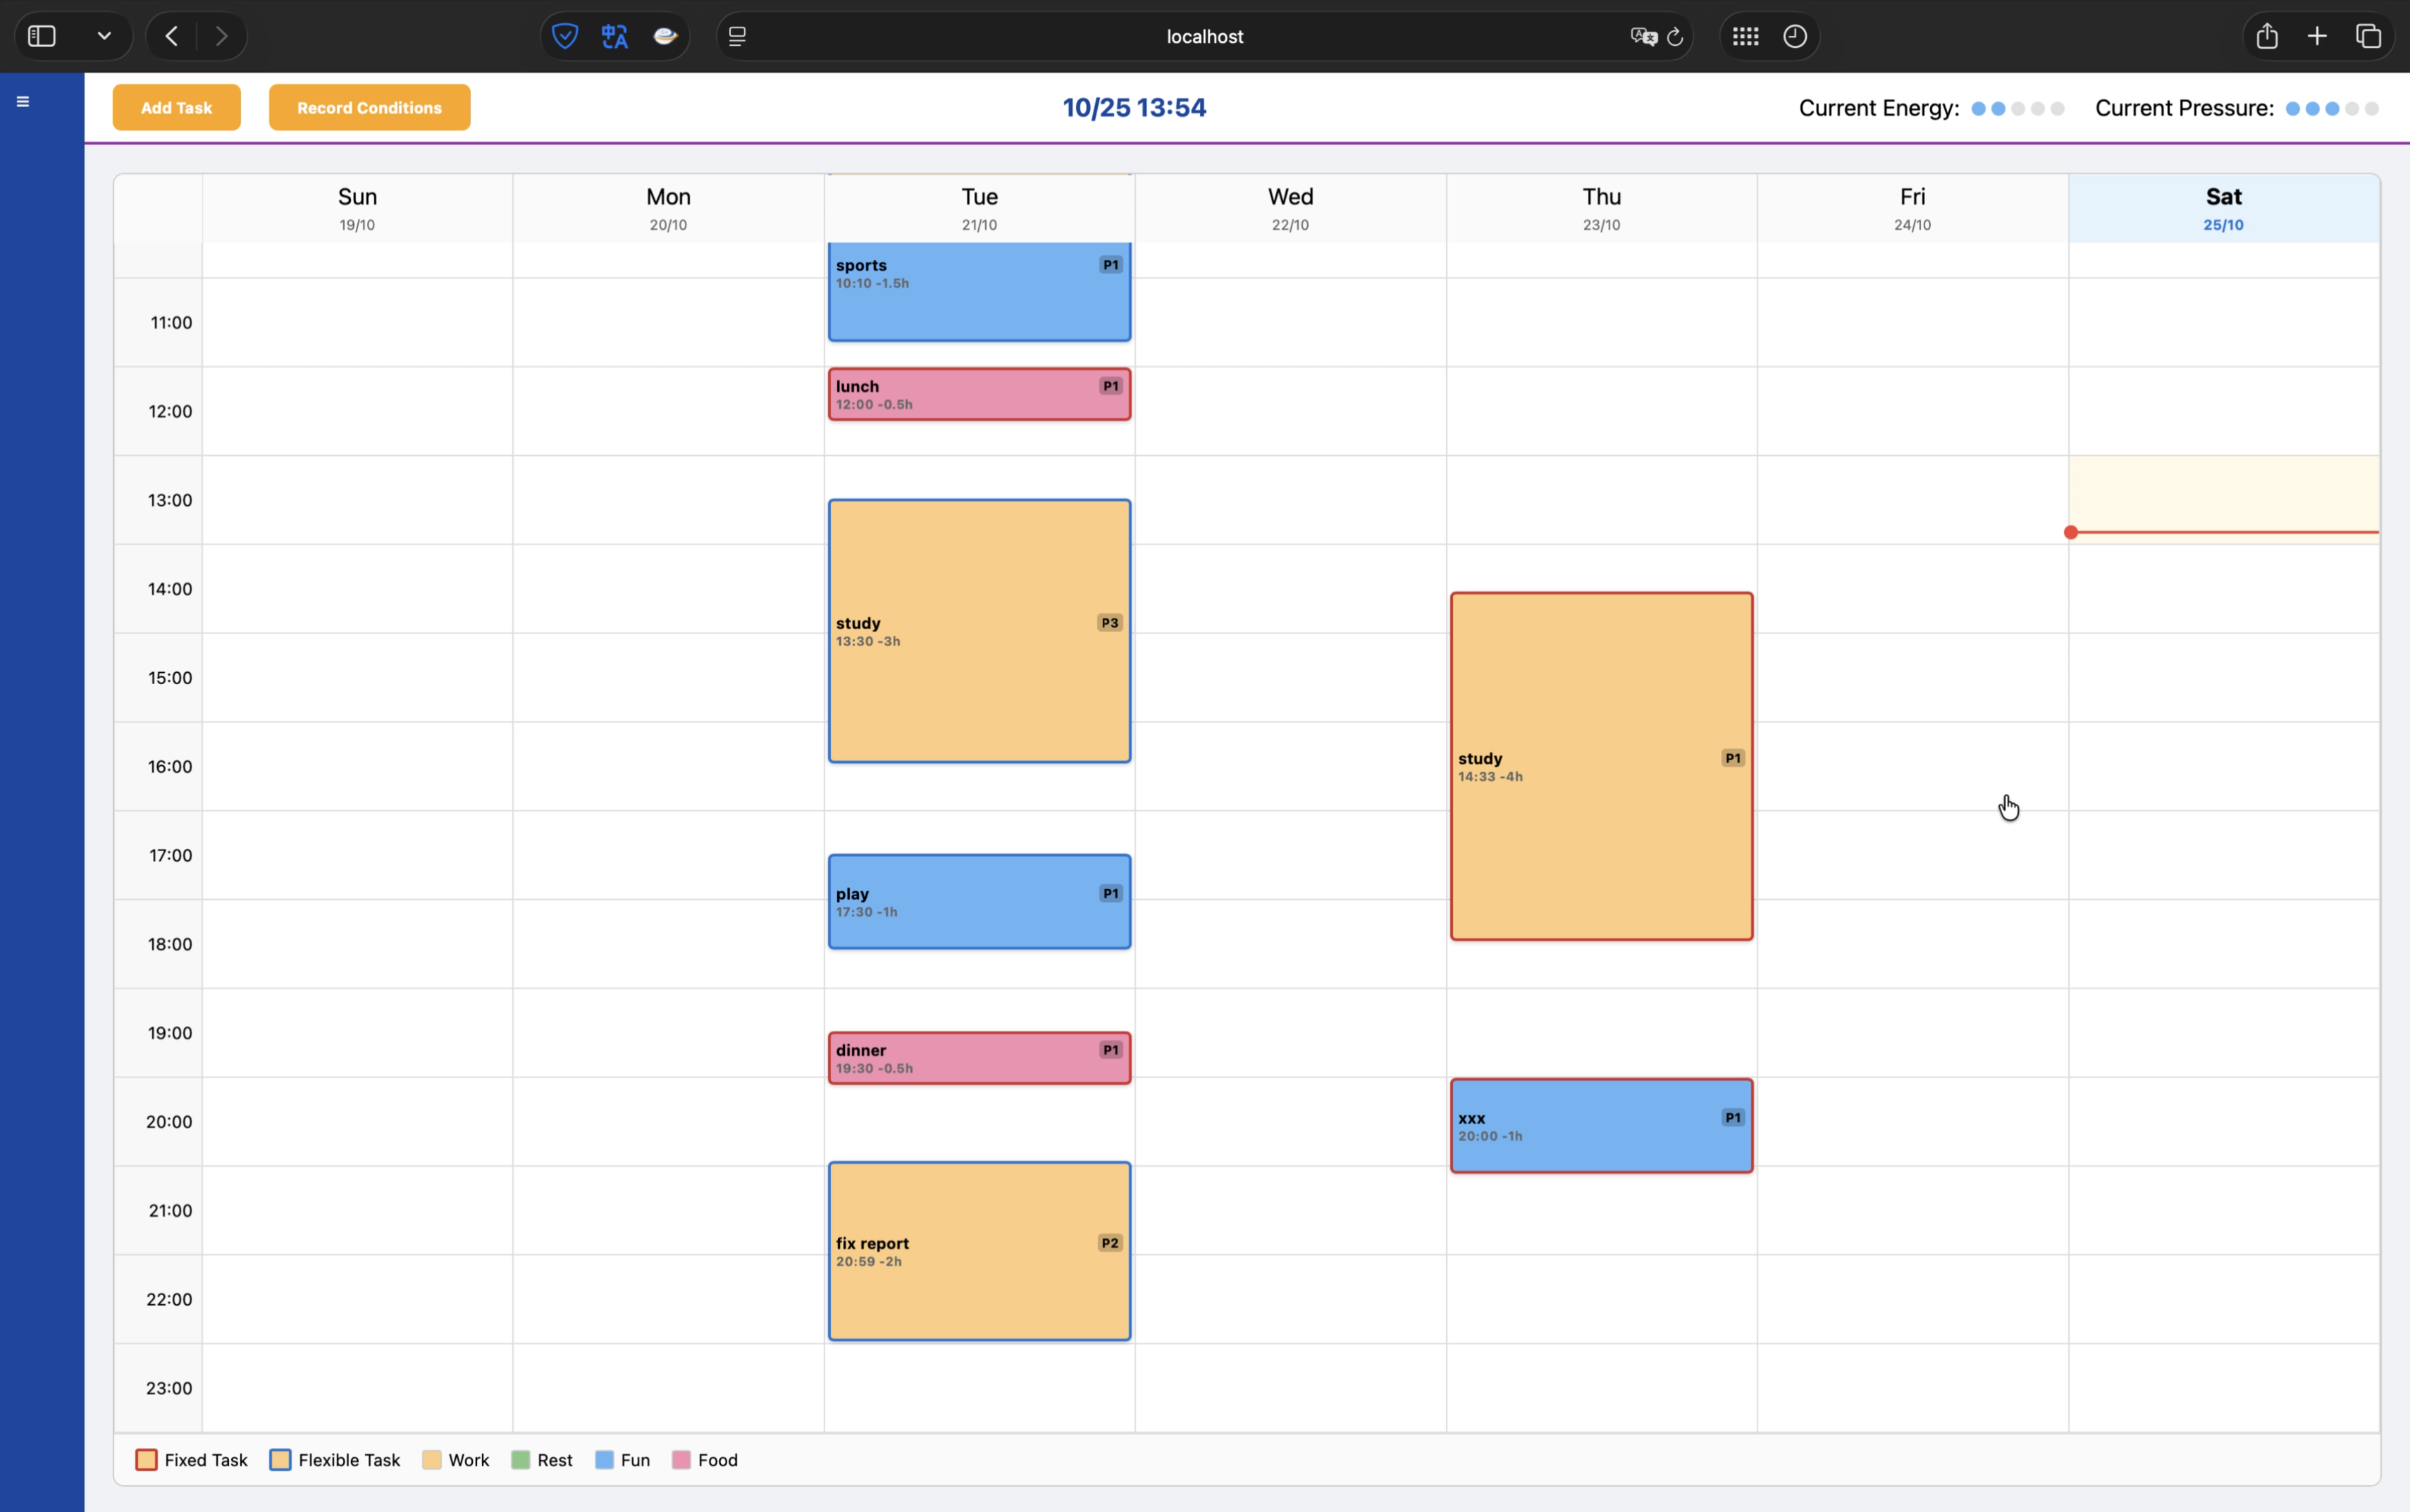
\includegraphics[width=\textwidth]{Images/System/timetable/aft_add.png}
                            \caption{After Adding Tasks}
                            \label{After Adding}
                        \end{minipage}
                    \end{figure}

                    \begin{figure}[H]
                        \begin{minipage}[t]{0.49\textwidth}
                            \centering
                            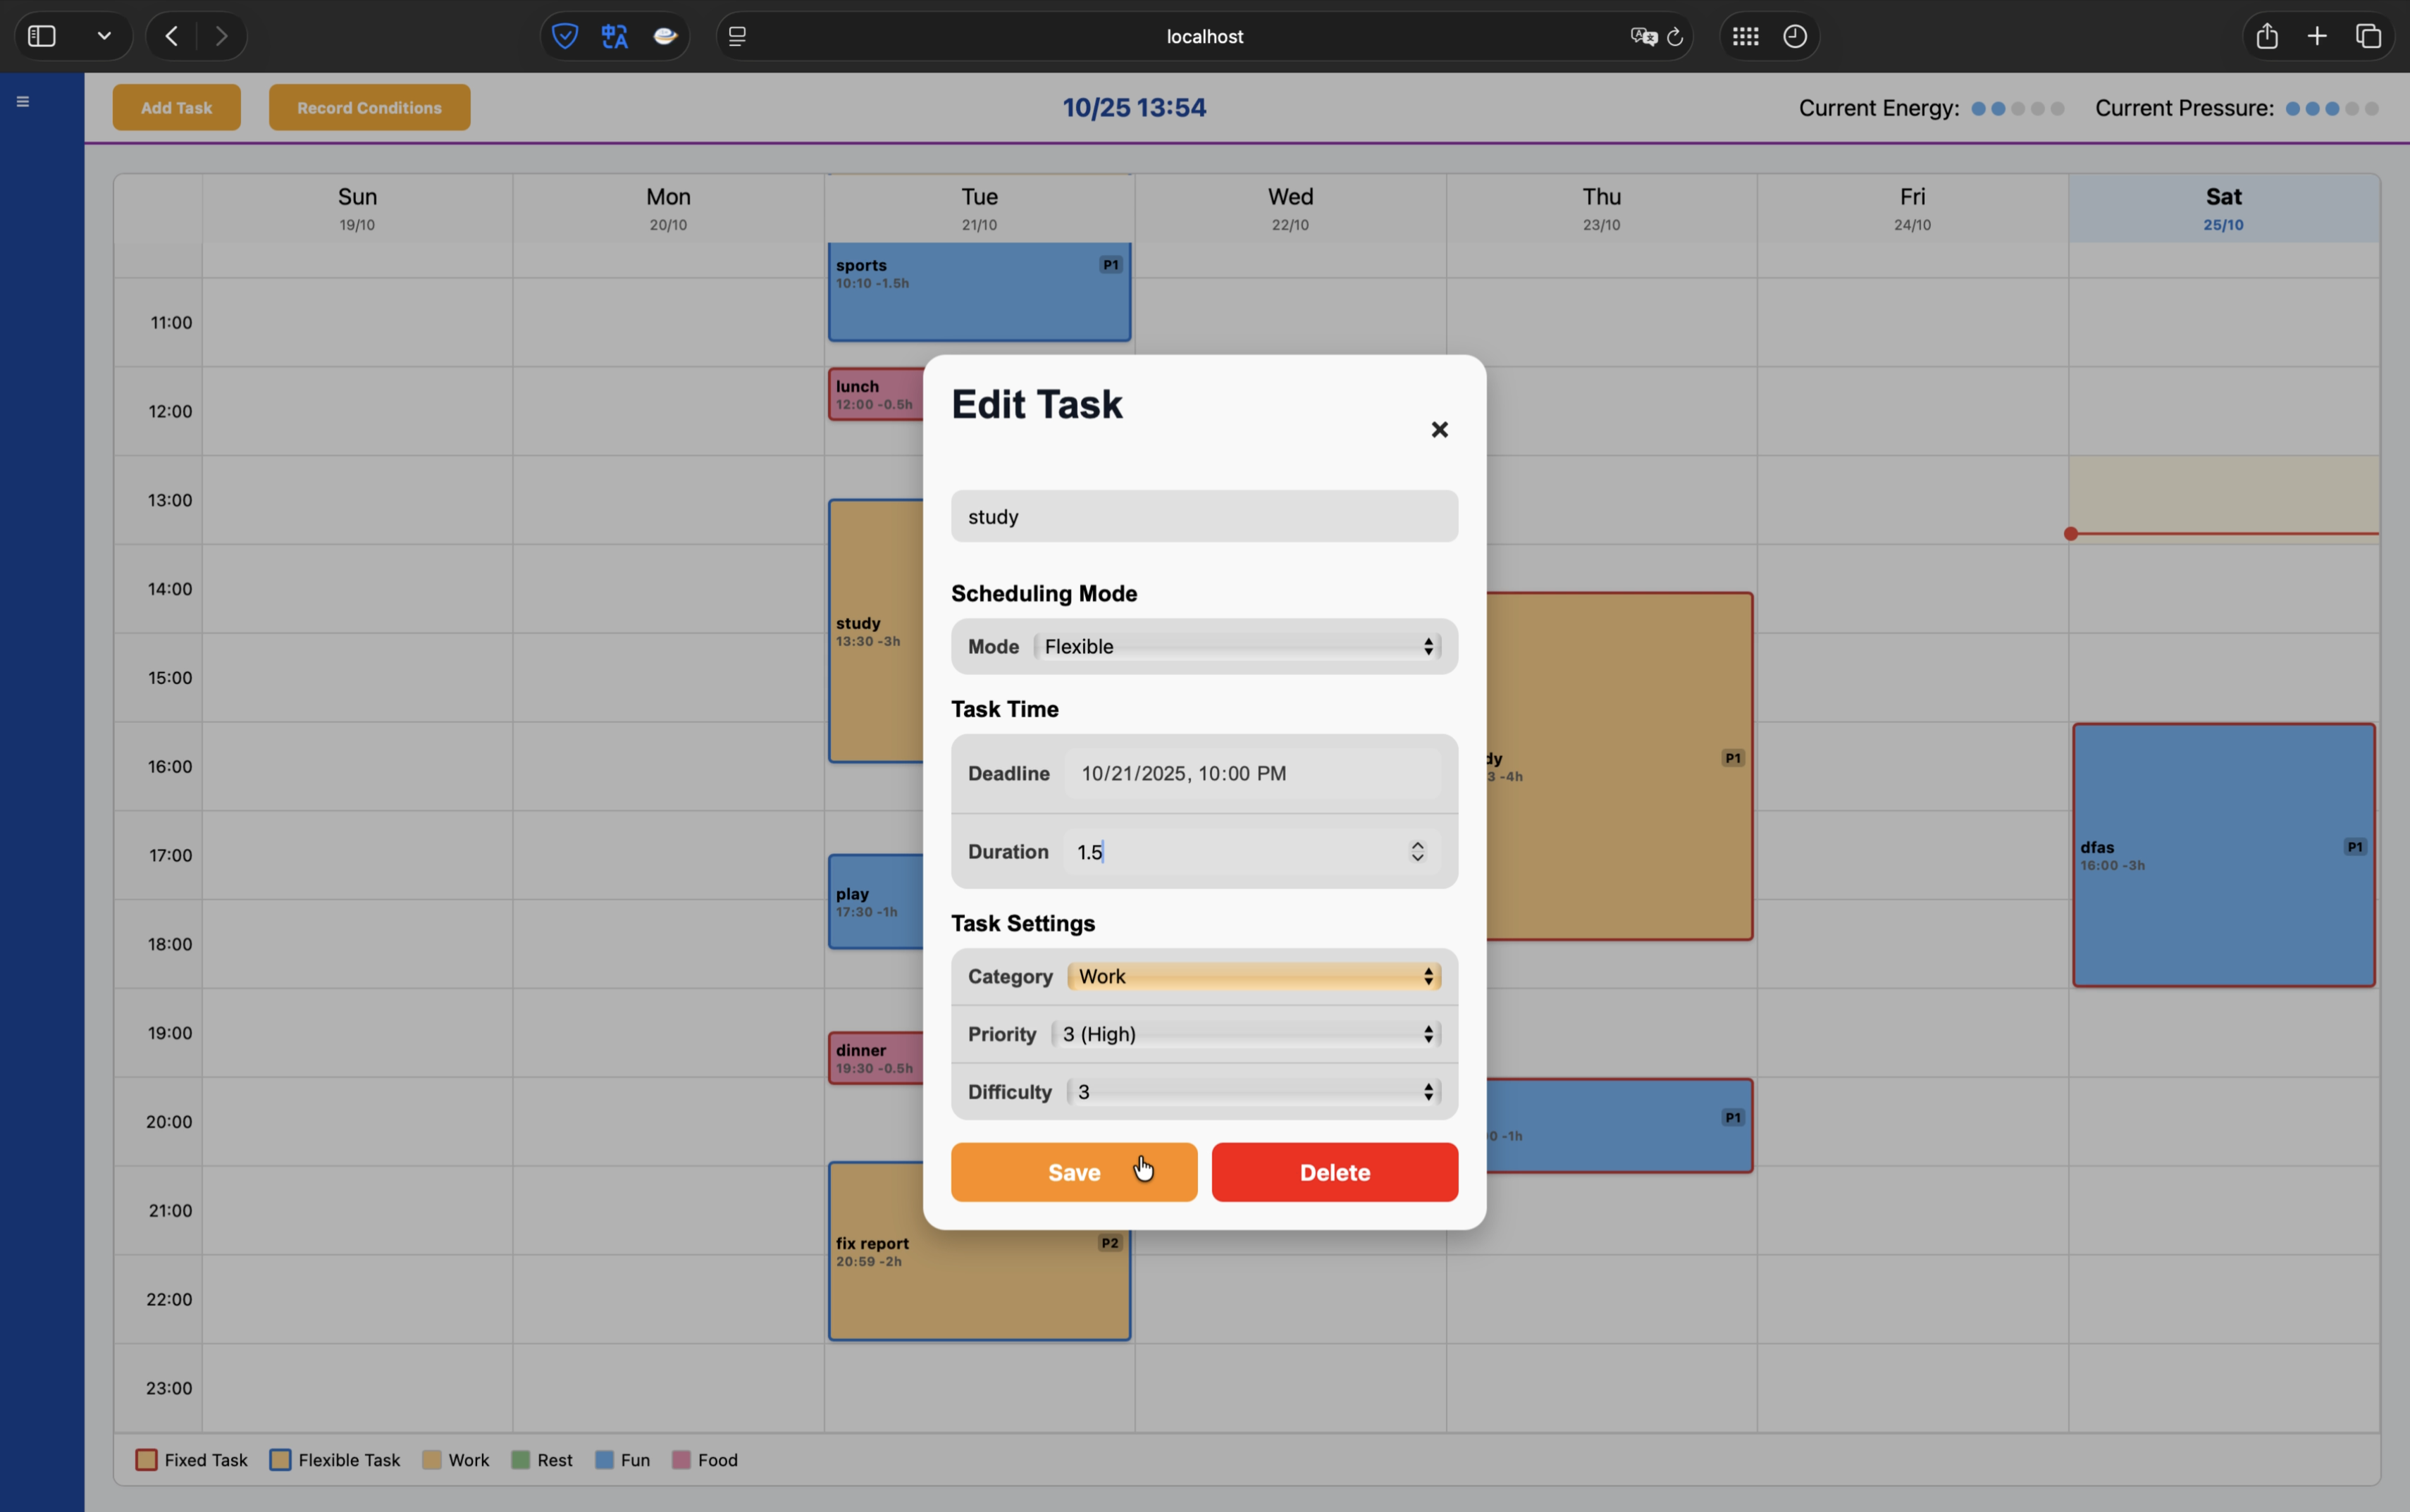
\includegraphics[width=\textwidth]{Images/System/timetable/change_duration.png}
                            \caption{Edit Duration of Tasks}
                            \label{change_duration}
                        \end{minipage}
                        \hfill
                        \begin{minipage}[t]{0.49\textwidth}
                            \centering
                            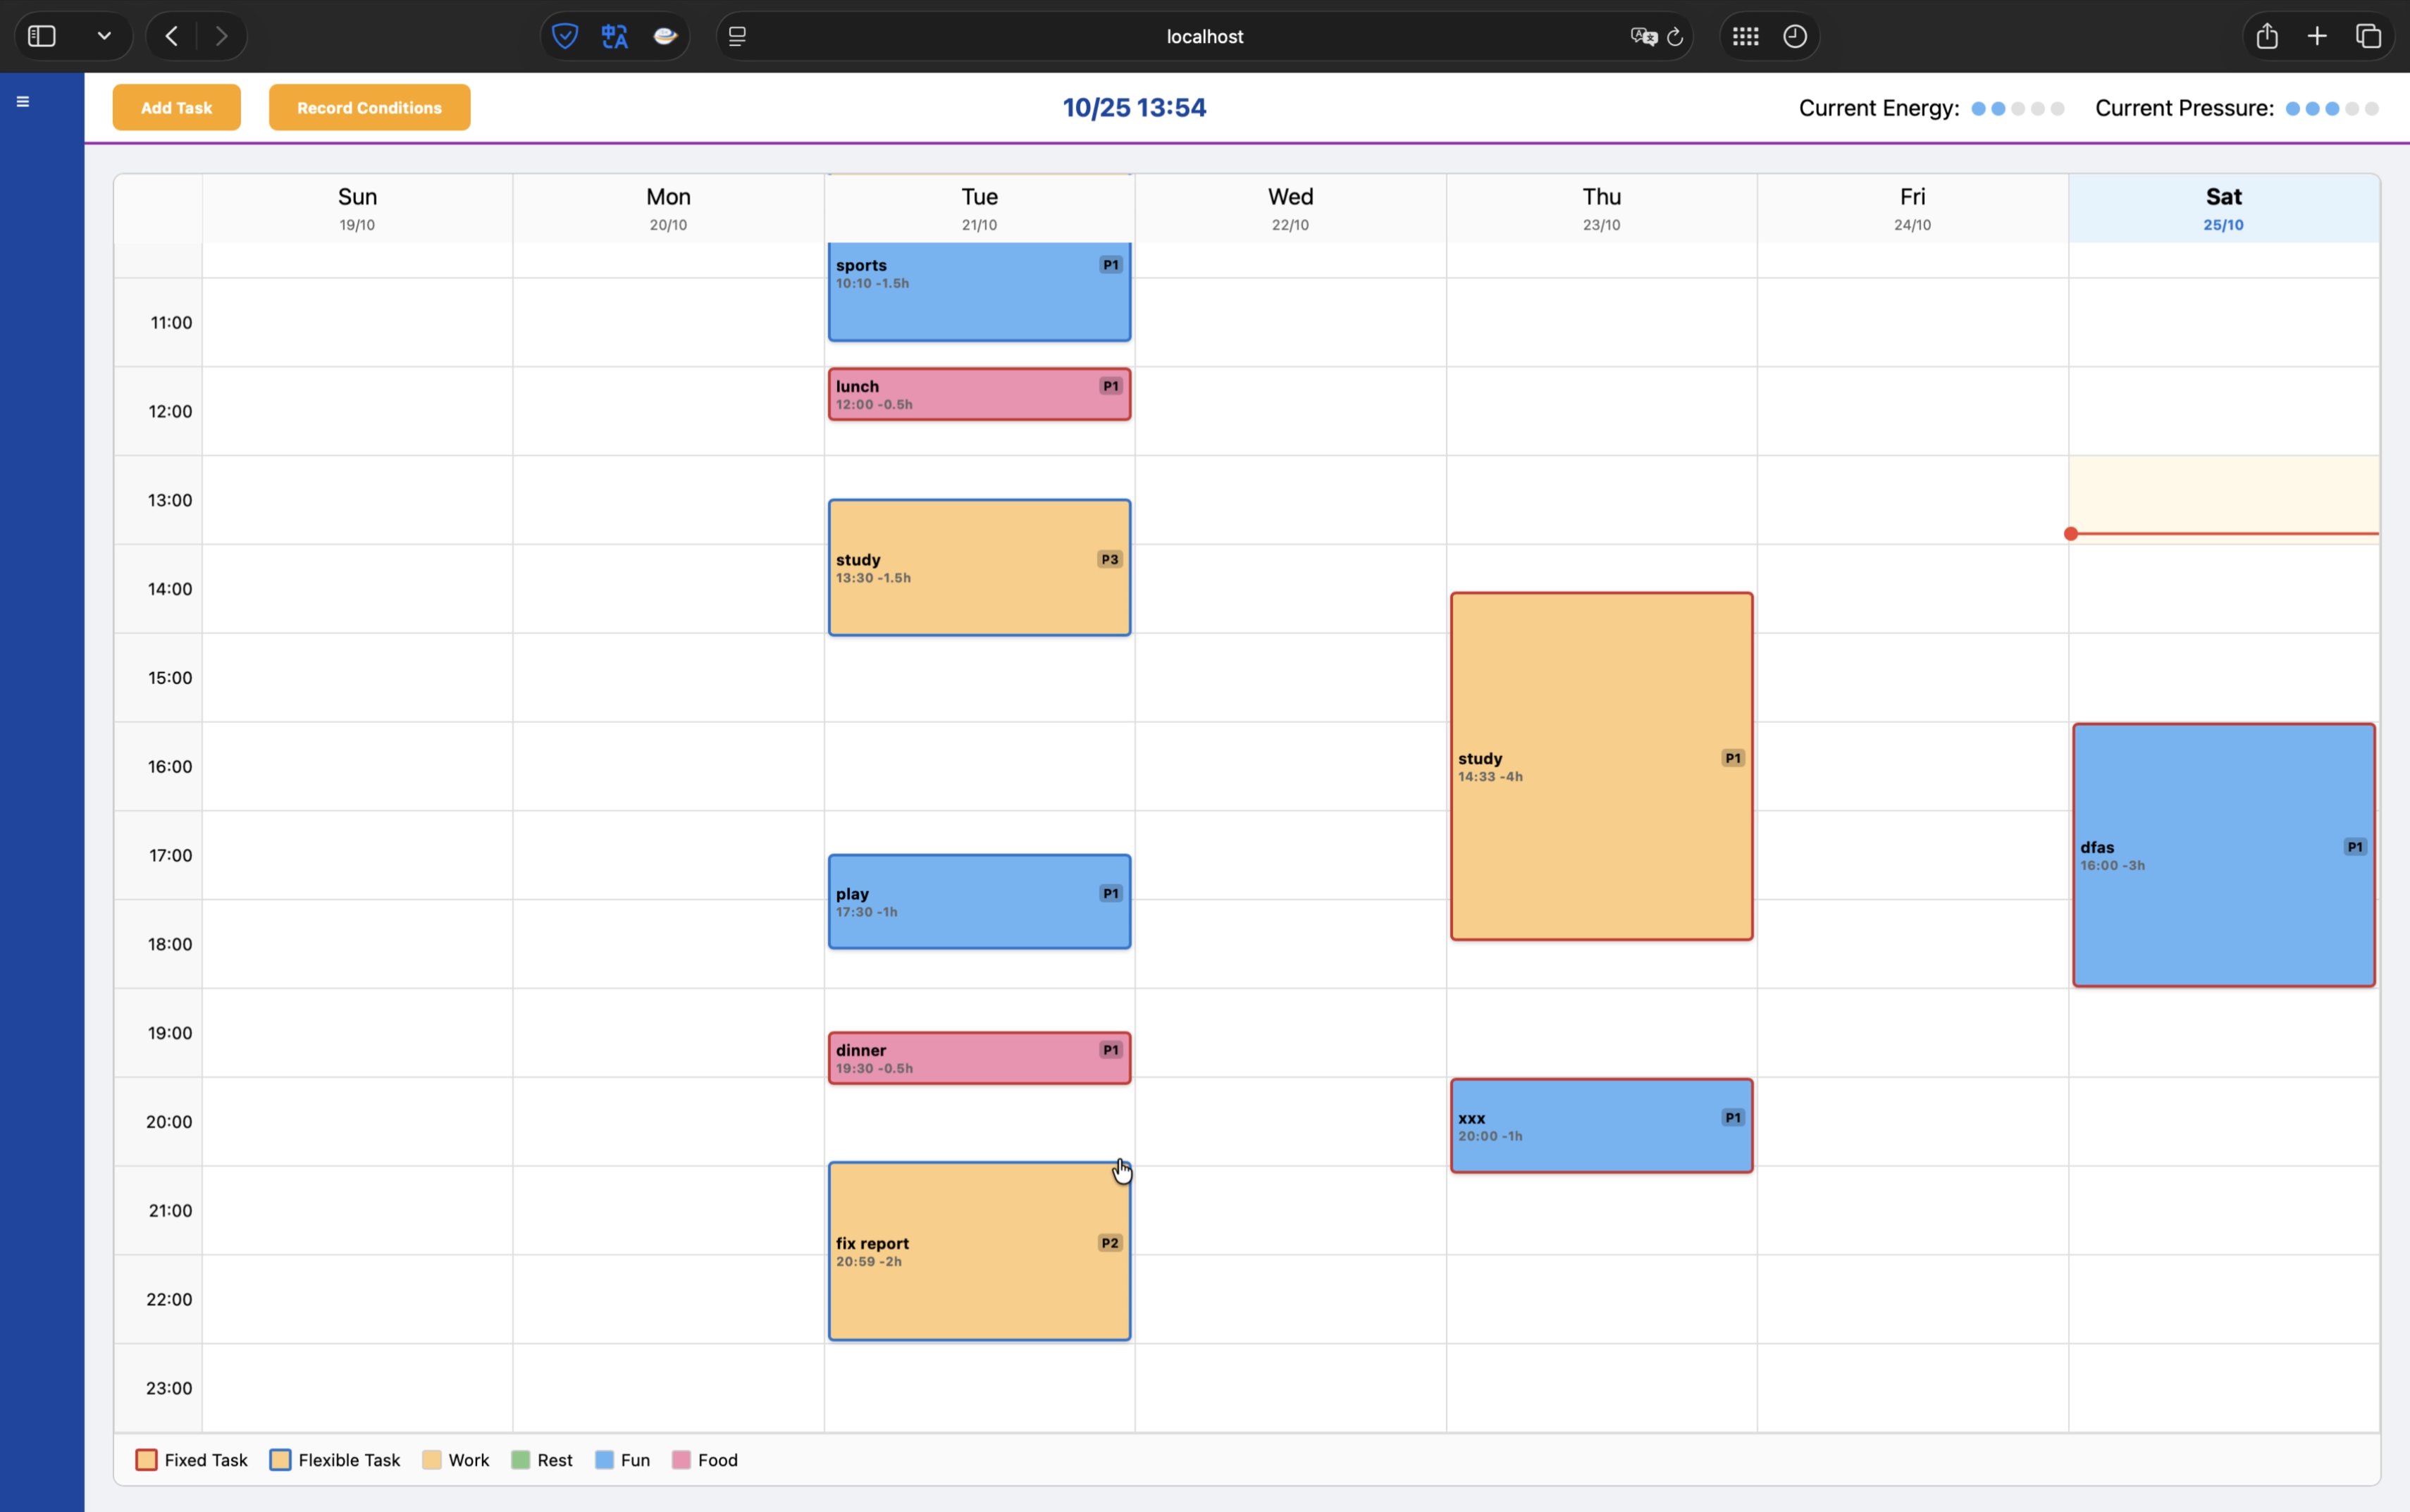
\includegraphics[width=\textwidth]{Images/System/timetable/aft_change_duration.png}
                            \caption{After Editing Duration}
                            \label{aft_change_duration}
                        \end{minipage}
                    \end{figure}

                    \begin{figure}[H]
                        \begin{minipage}[t]{0.49\textwidth}
                            \centering
                            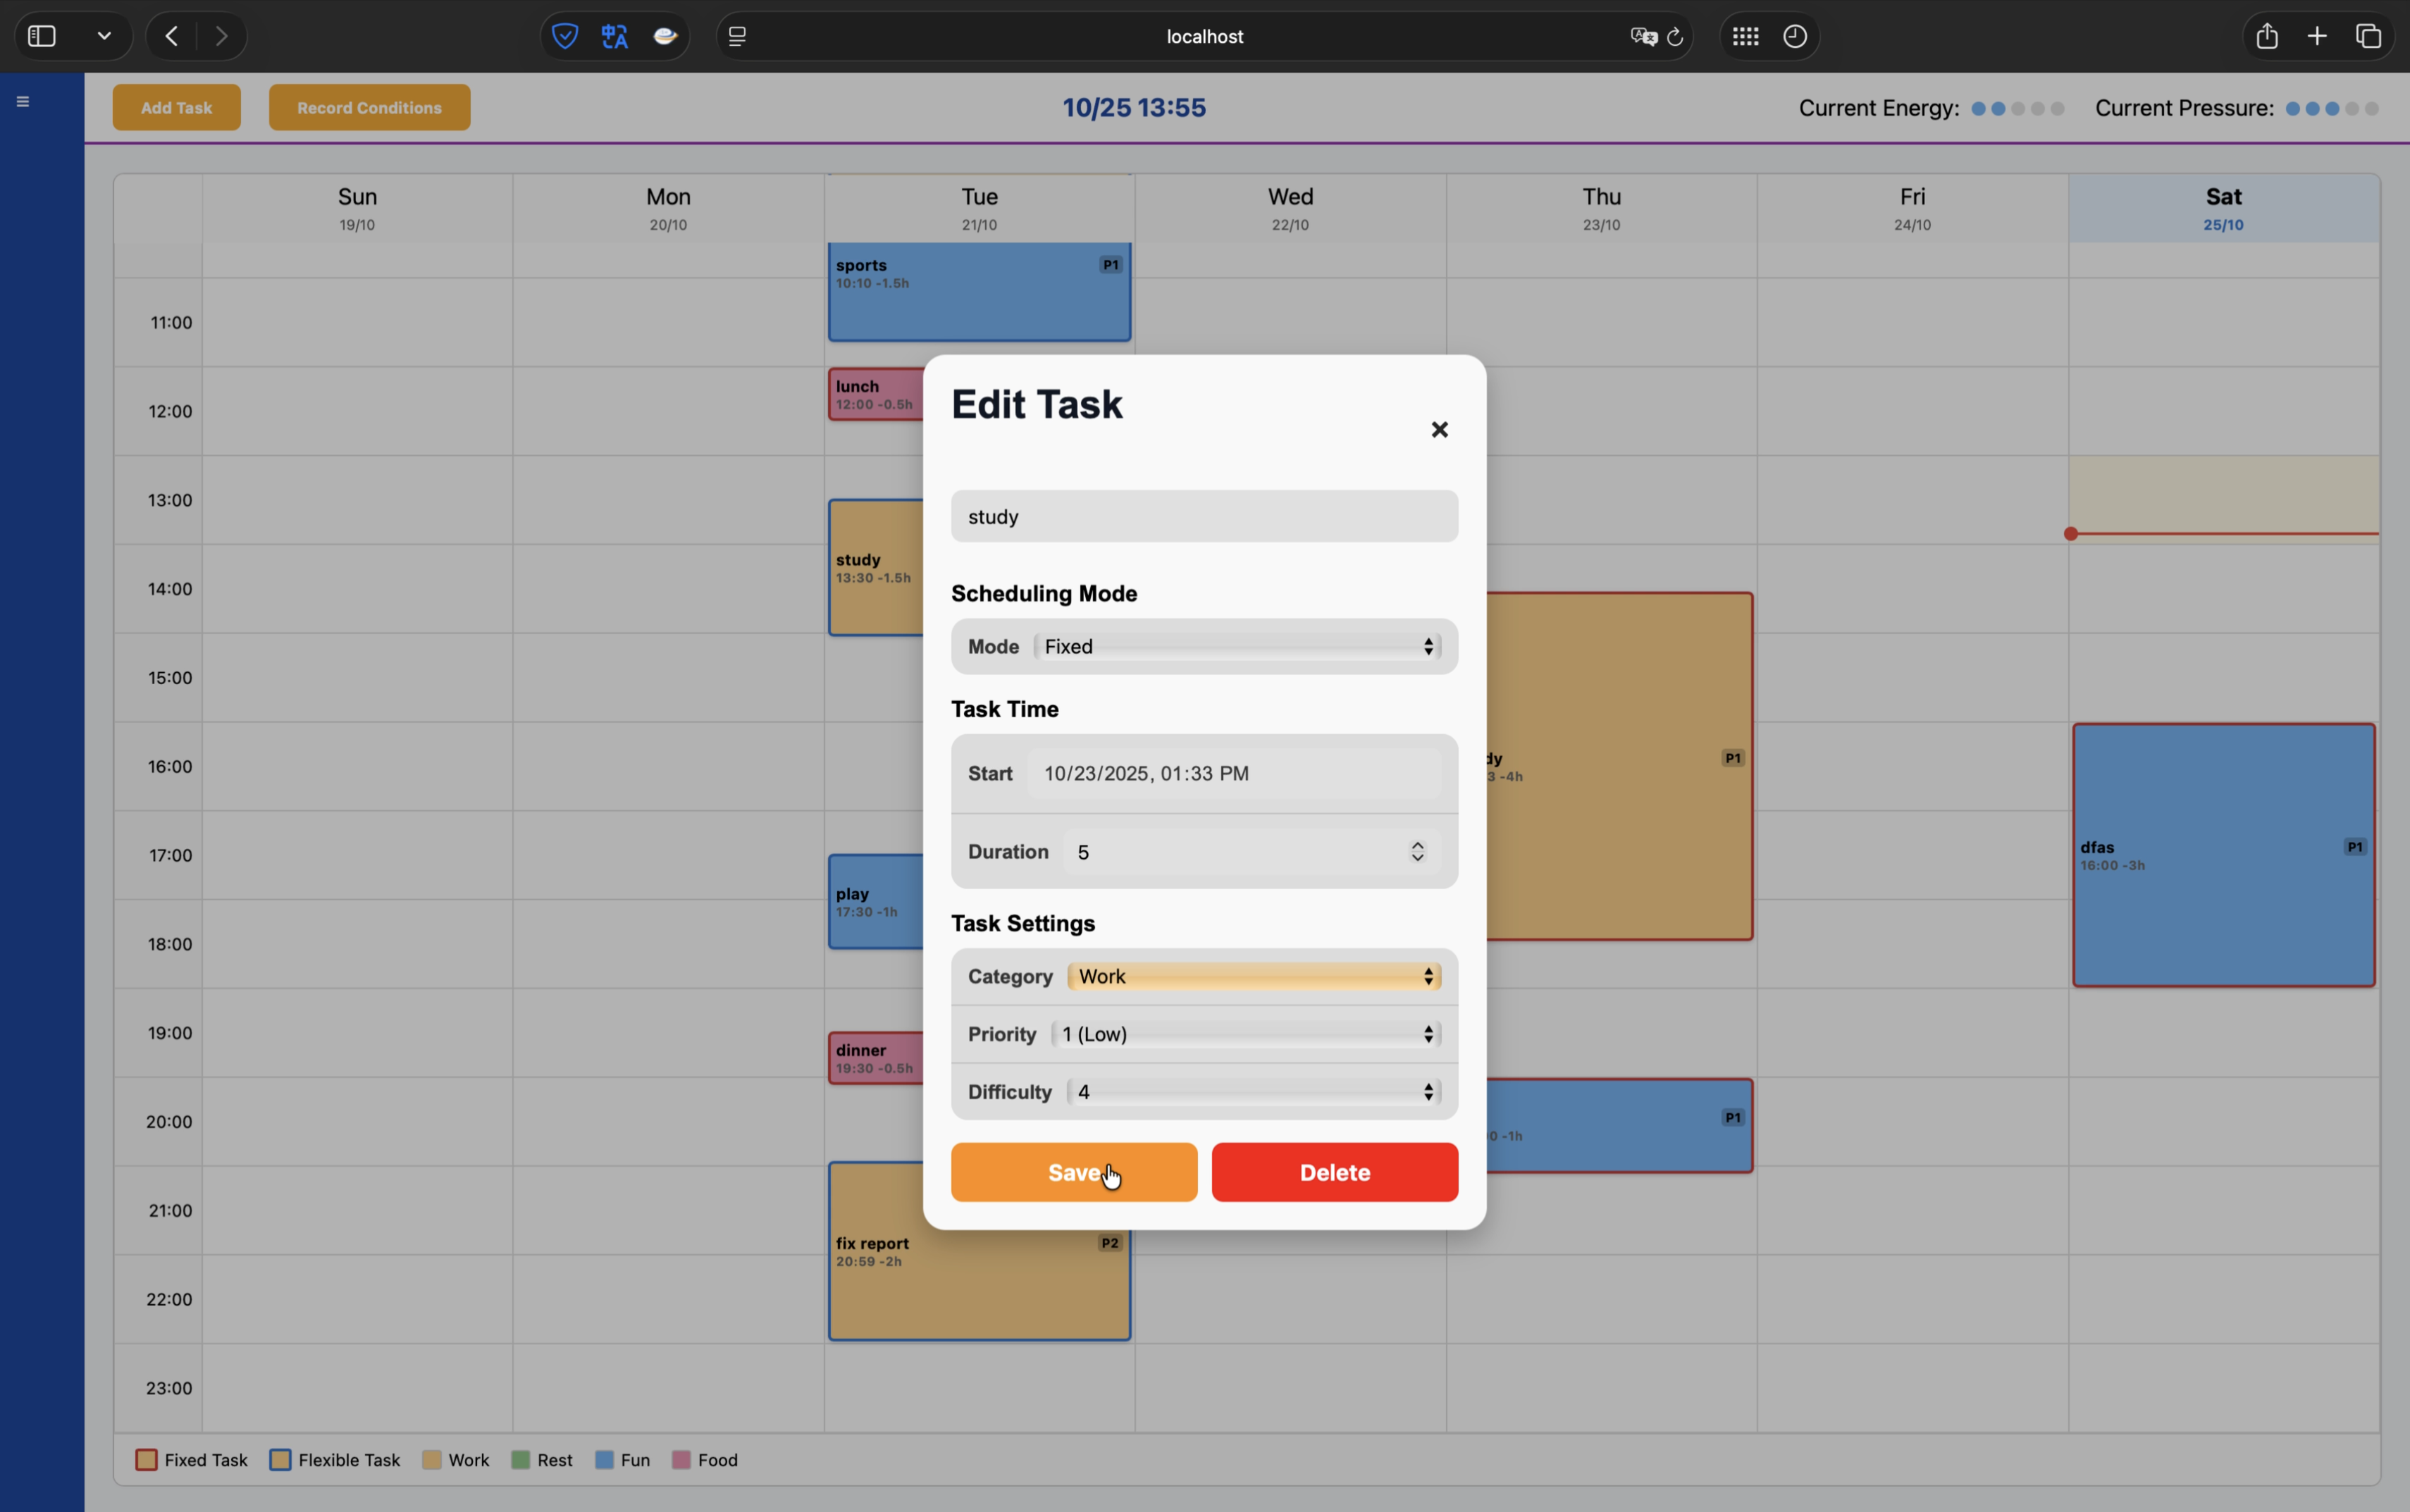
\includegraphics[width=\textwidth]{Images/System/timetable/change_starttime.png}
                            \caption{Edit Start Time of Tasks}
                            \label{change_starttime}
                        \end{minipage}
                        \hfill
                        \begin{minipage}[t]{0.49\textwidth}
                            \centering
                            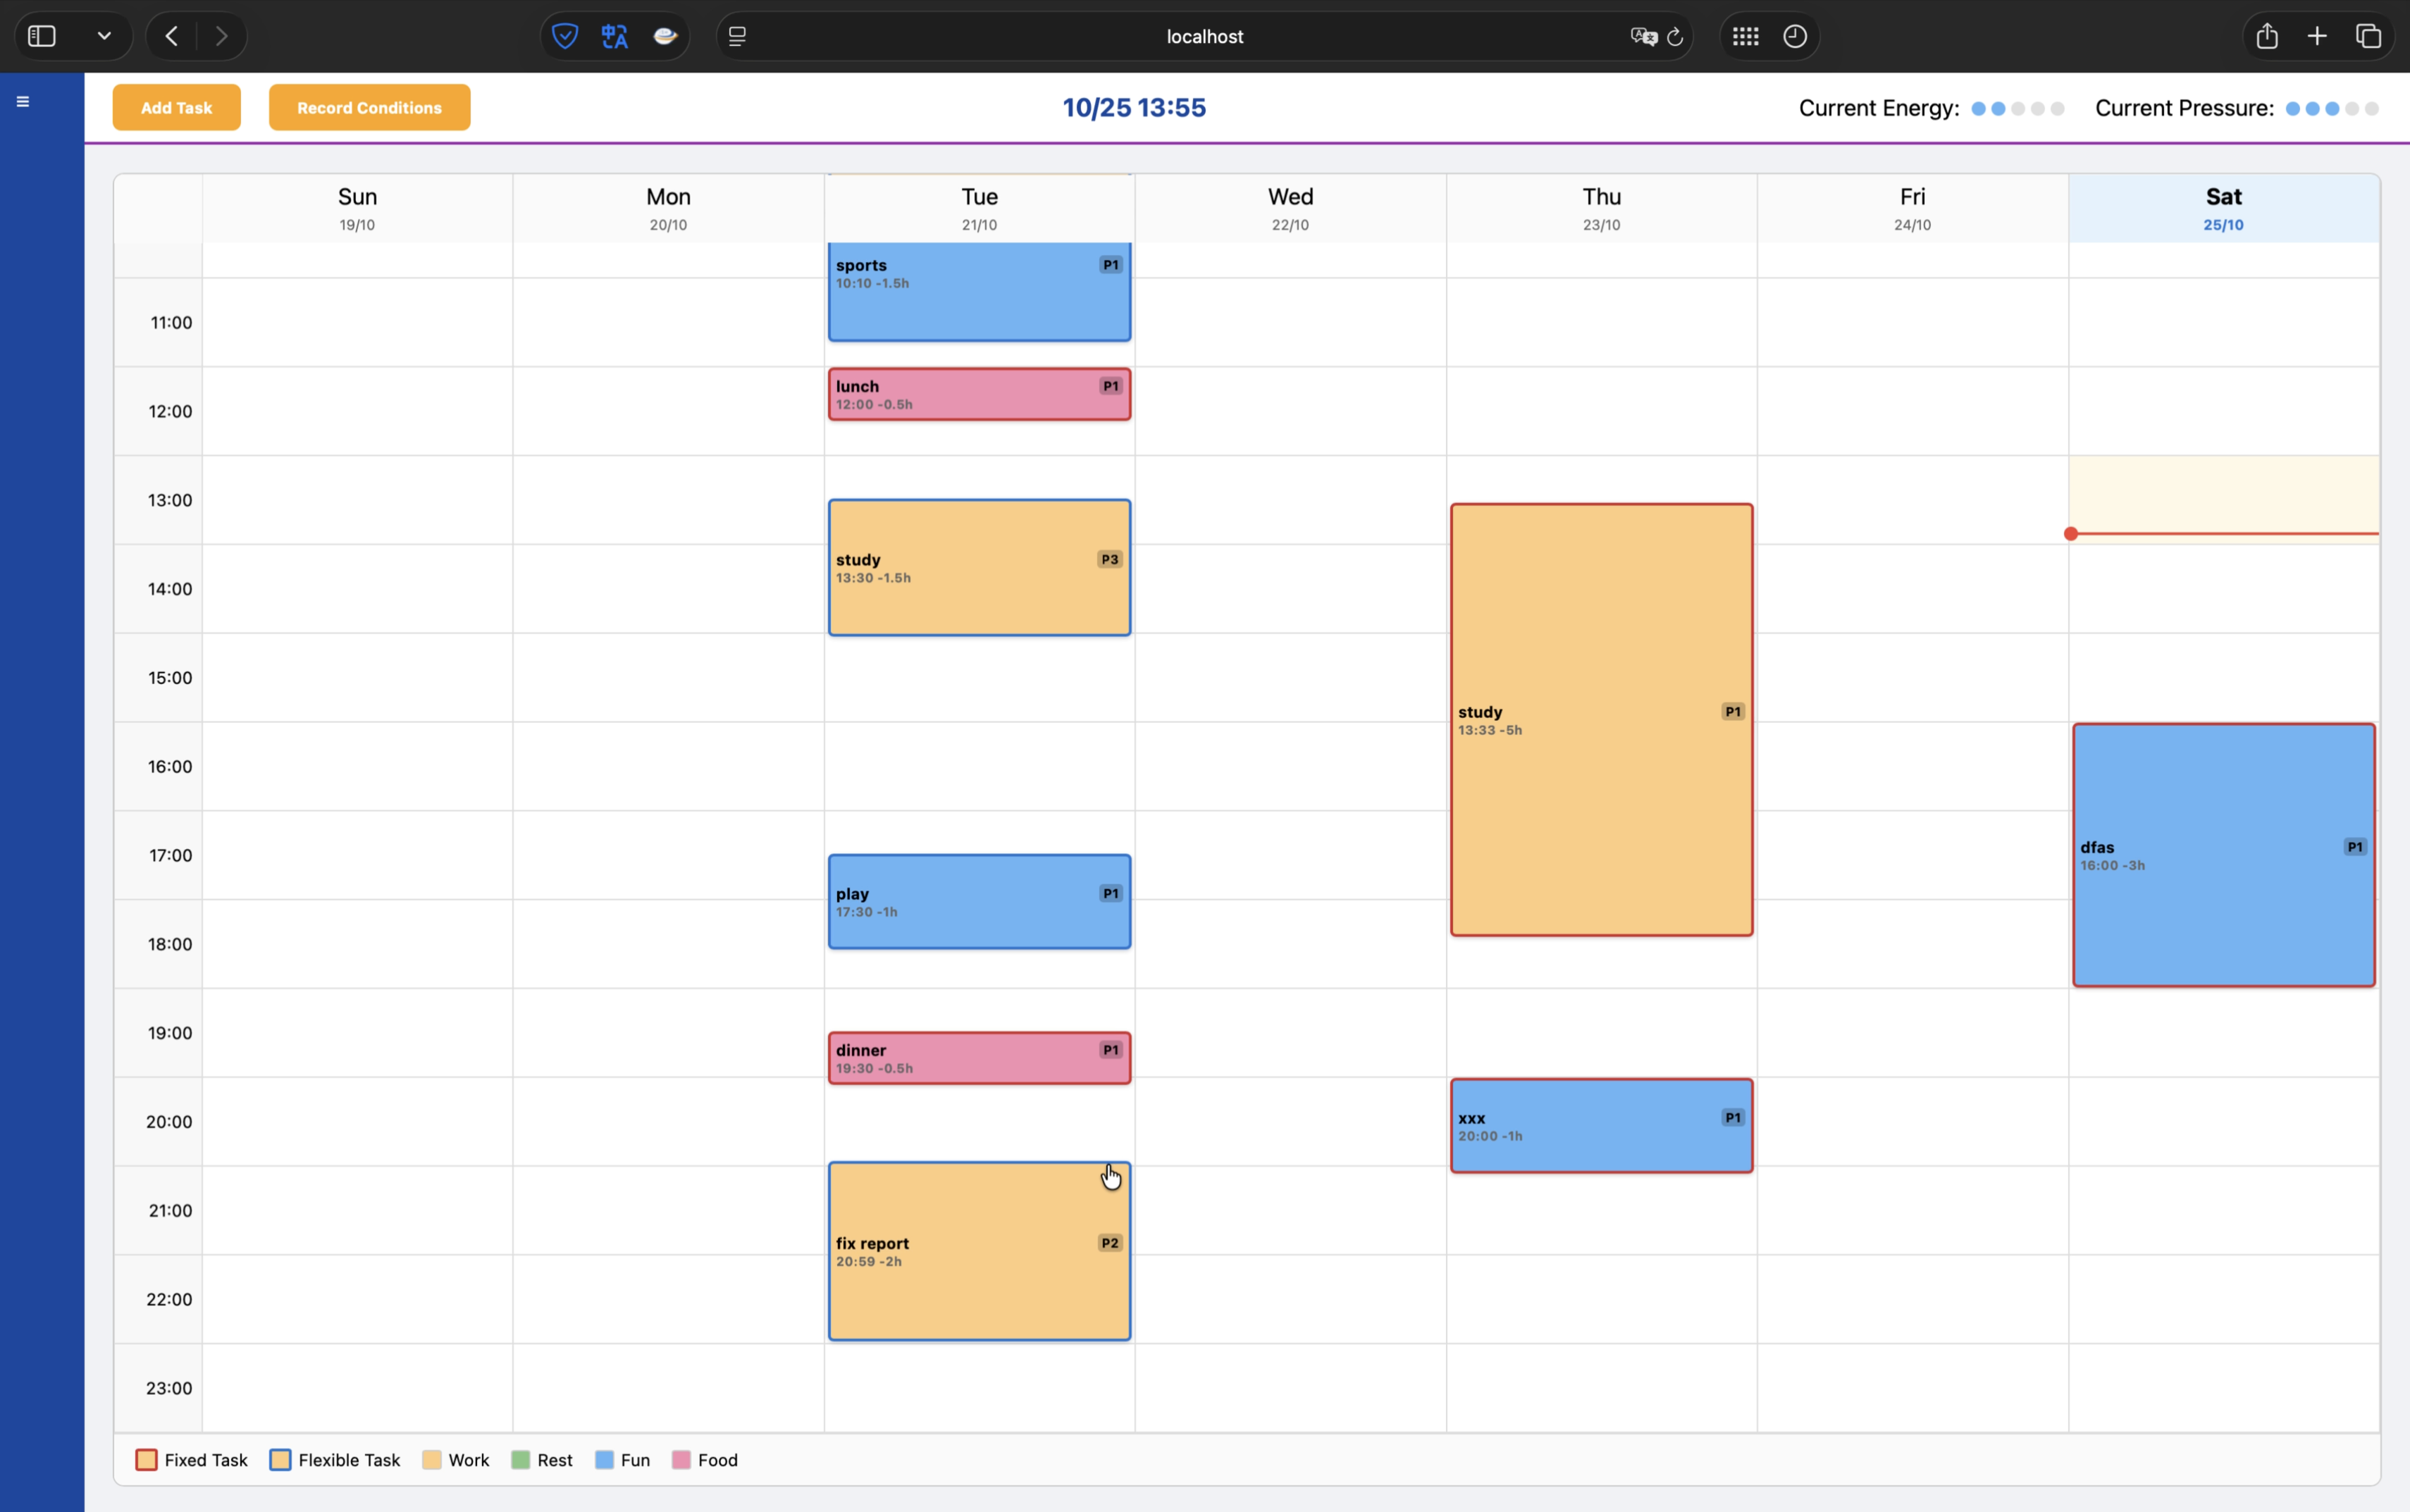
\includegraphics[width=\textwidth]{Images/System/timetable/aft_change_starttime.png}
                            \caption{After Editing Start Time}
                            \label{aft_change_starttime}
                        \end{minipage}
                    \end{figure}

                    \begin{figure}[H]
                        \begin{minipage}[t]{0.49\textwidth}
                            \centering
                            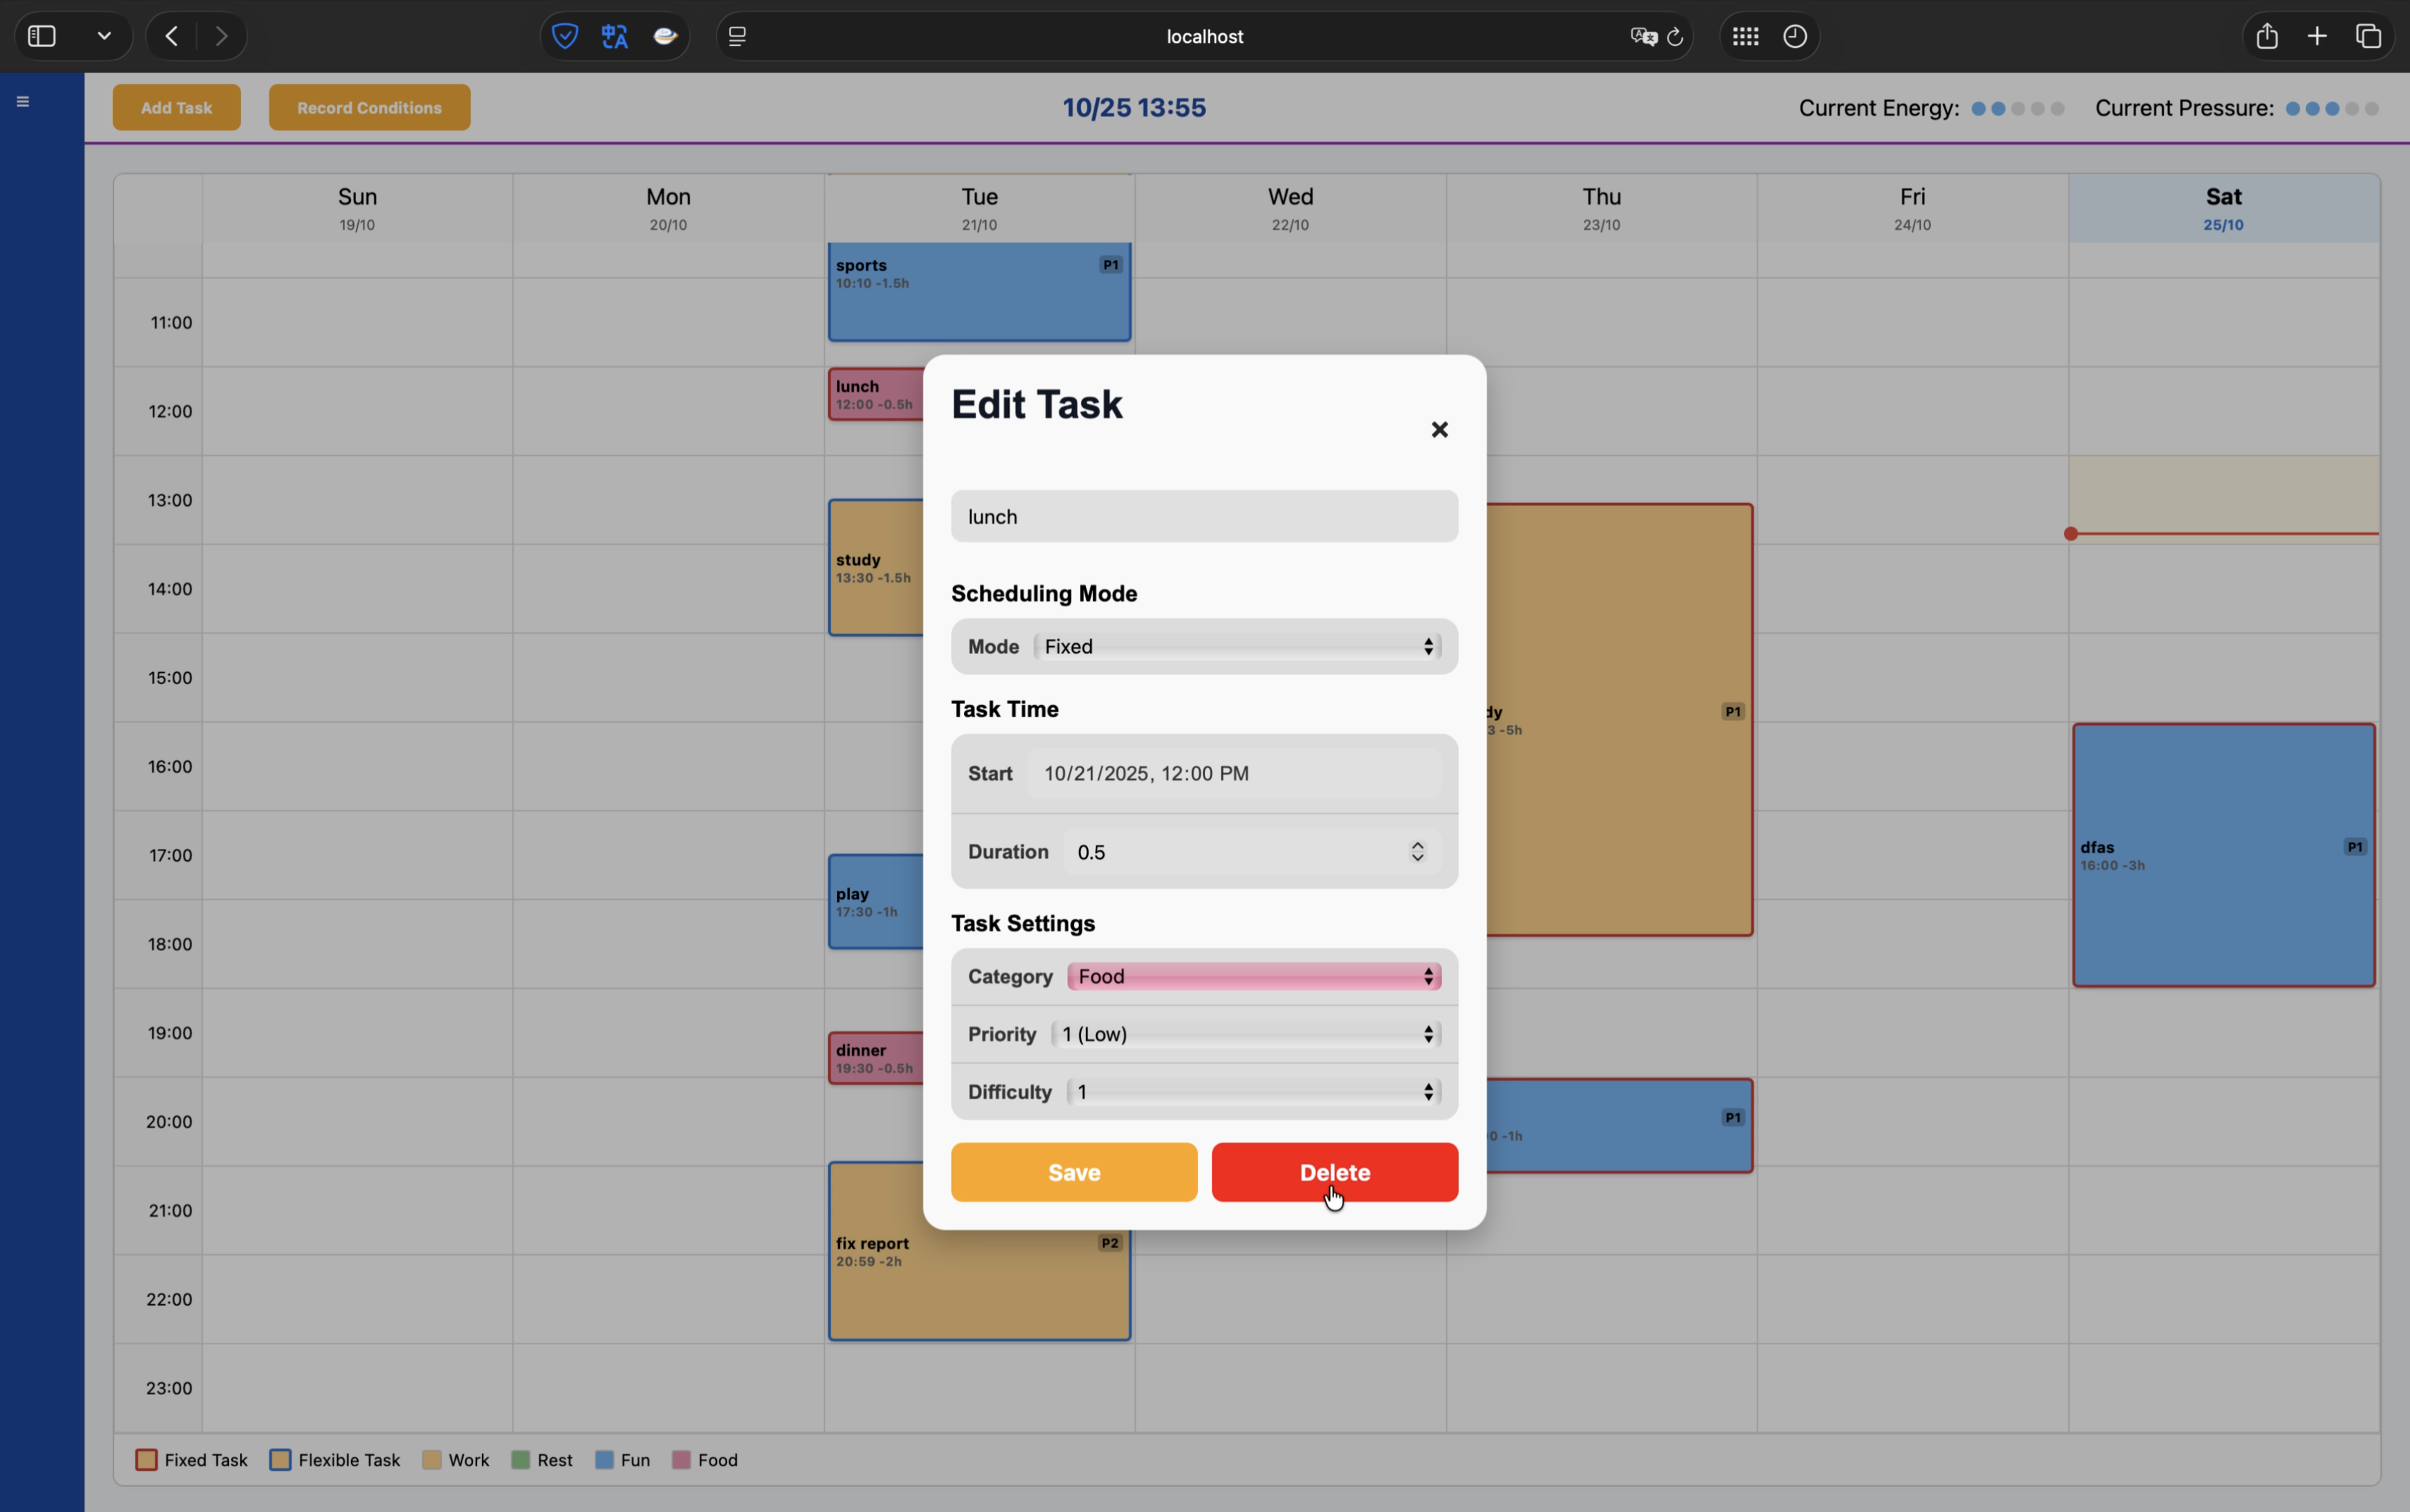
\includegraphics[width=\textwidth]{Images/System/timetable/delete.png}
                            \caption{Delete Tasks}
                            \label{delete}
                        \end{minipage}
                        \hfill
                        \begin{minipage}[t]{0.49\textwidth}
                            \centering
                            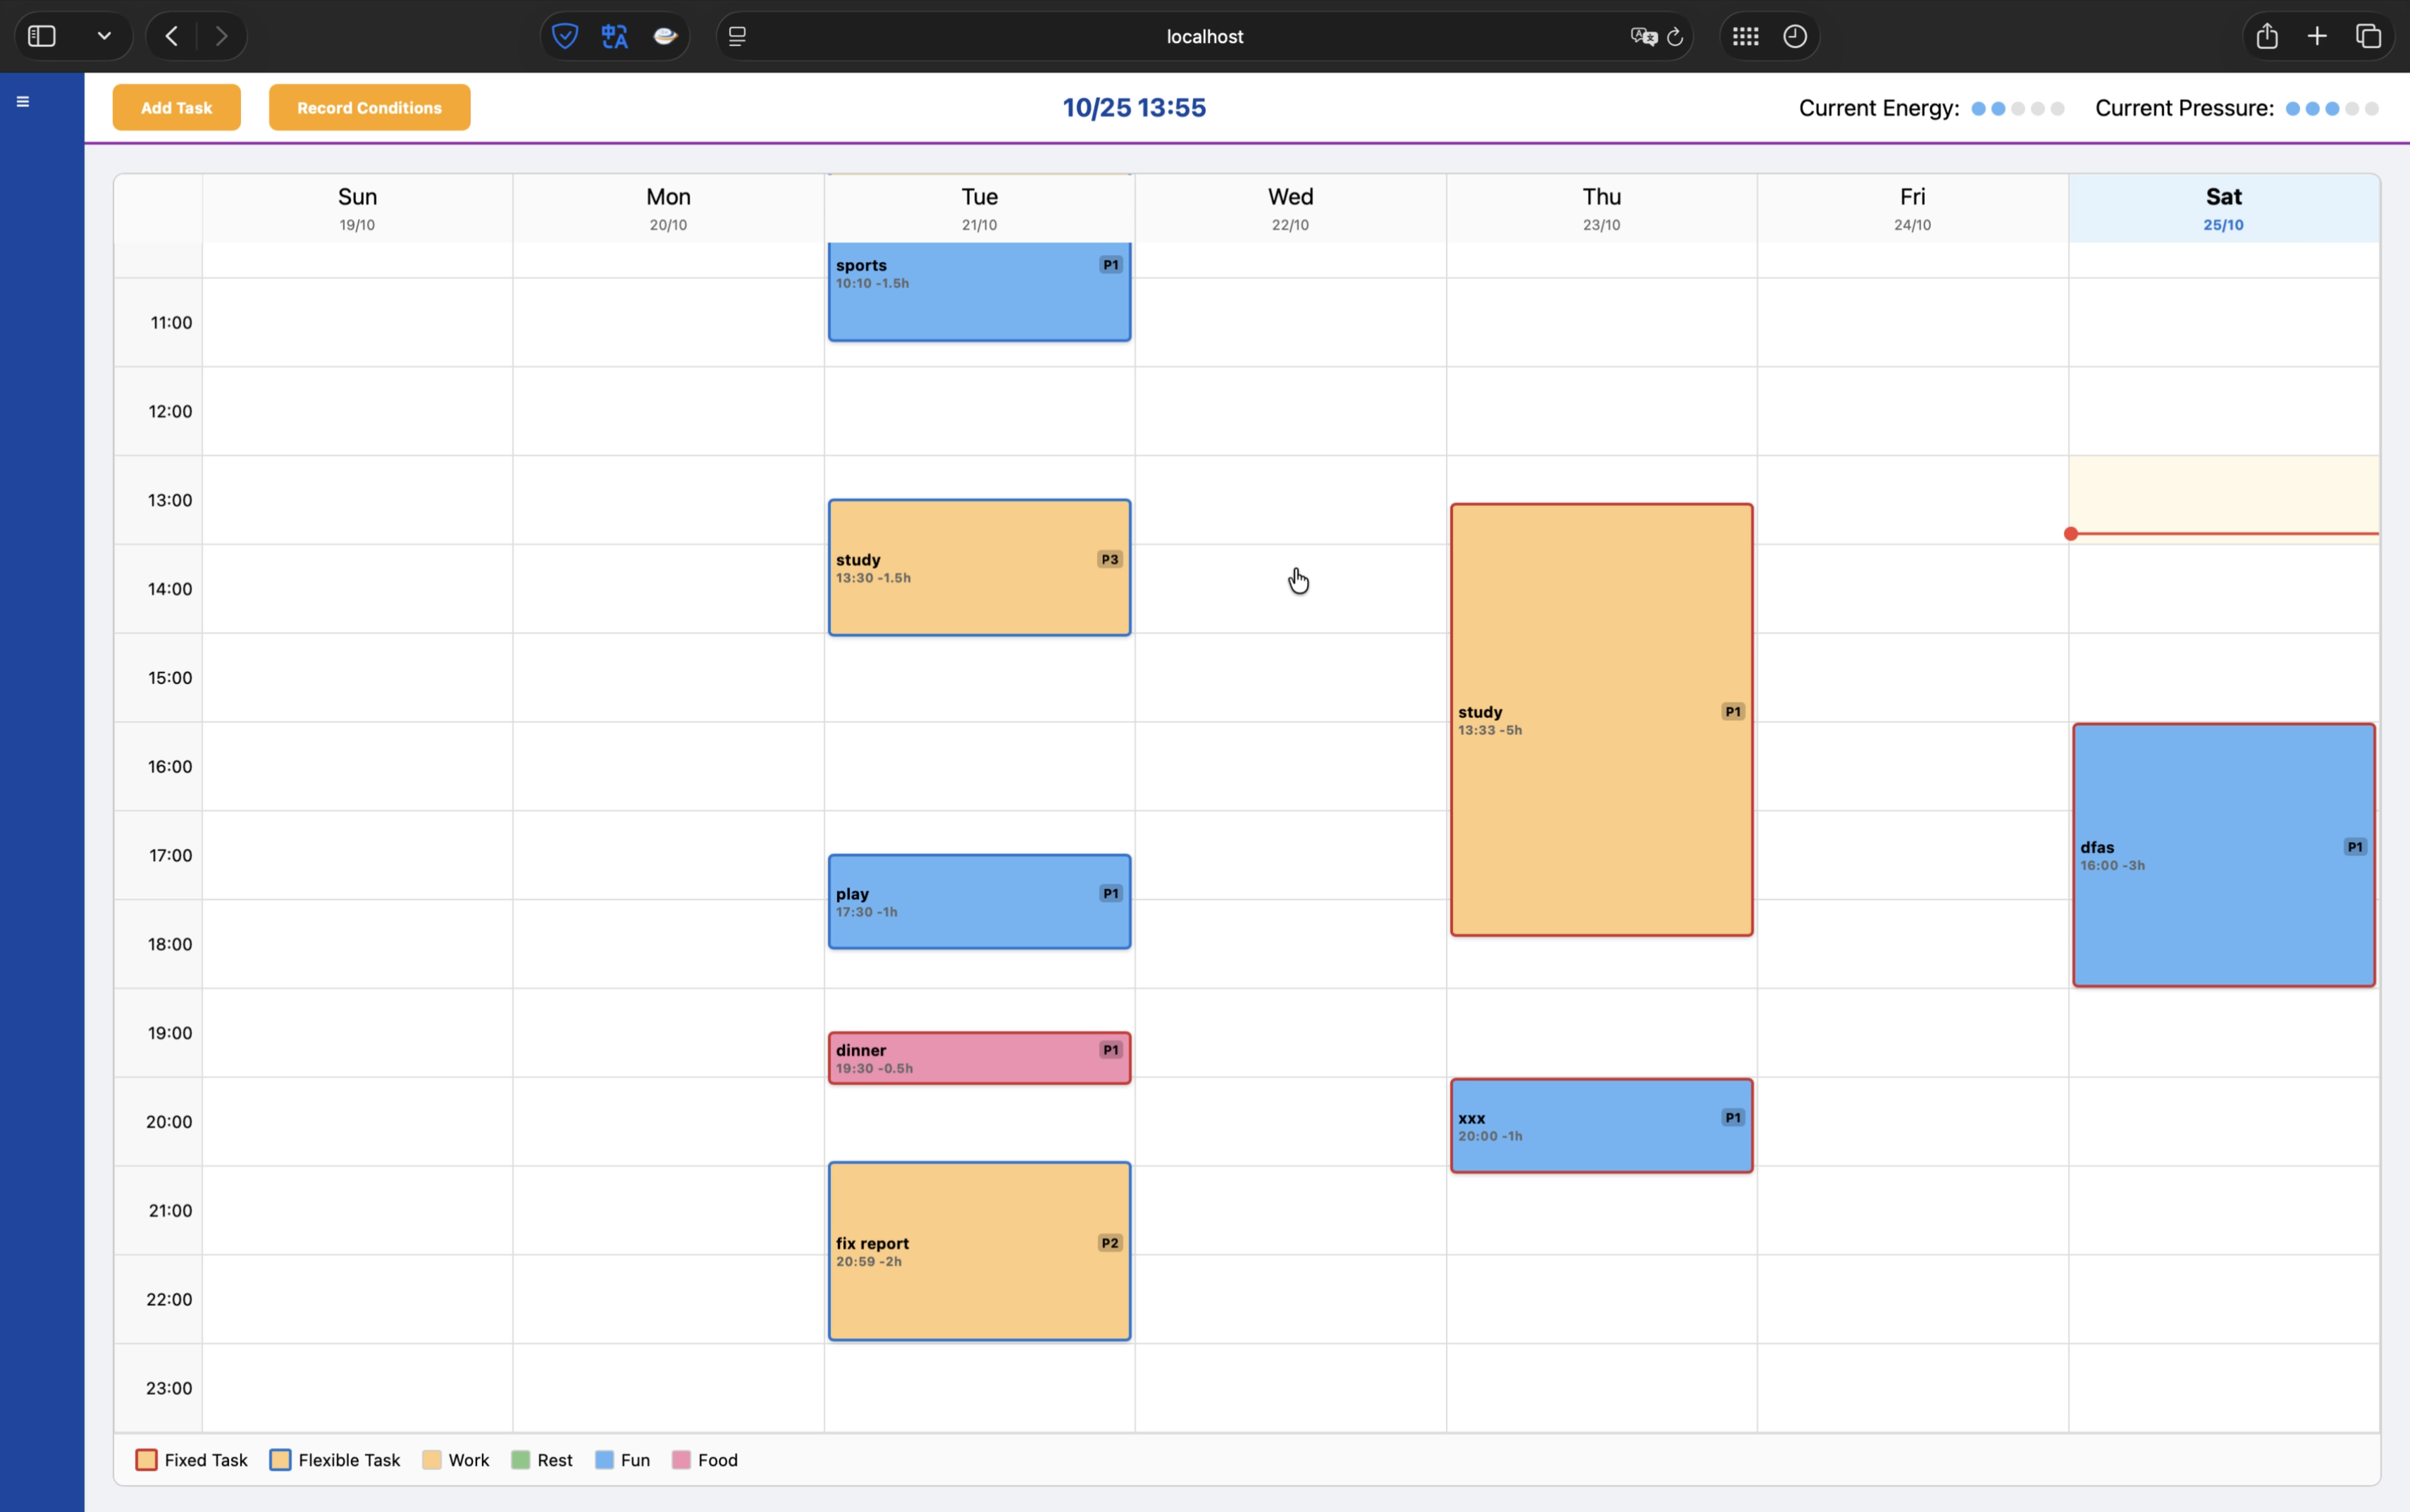
\includegraphics[width=\textwidth]{Images/System/timetable/aft_delete.png}
                            \caption{After Deleting}
                            \label{aft_delete}
                        \end{minipage}
                    \end{figure}

                \item \textbf{AI Scheduling}

                    In the Timetable and Today’s Tasks pages, users can add \textbf{flexible tasks} (Figure~\ref{add_flex}) and delegate scheduling to the system. Upon submission, the pretrained evaluation model (see \textbf{Task Evaluation Model}) estimates each task’s energy and pressure costs. When the user clicks \emph{Run Intelligent Scheduling}, the scheduler allocates all flexible tasks to feasible time slots subject to constraints (e.g., working hours, existing commitments, and rest buffers). Upon success, a confirmation dialog 

                    \begin{quote}
                        \textit{“Intelligent scheduling executed! ”}
                    \end{quote}
                    
                    is displayed (Figure~\ref{sch_succ}). The resulting plan appears on the Today’s Tasks page (Figure~\ref{aft_sch_todaytask}) and in the weekly overview on the Dashboard (Figure~\ref{aft_scheduling}). The AI-scheduling workflow is summarized below.
                    
                    \begin{itemize}
                        \item User submits one or more flexible tasks.
                        \item The evaluation model predicts energy and pressure costs for each task.
                        \item The scheduler formulates a constrained allocation problem over available time slots.
                        \item A solver assigns tasks, inserts rest buffers, and resolves conflicts by priority/difficulty.
                        \item On success, the plan is committed and surfaced to the UI; otherwise, the user is prompted to revise inputs.
                    \end{itemize}


                    \begin{figure}[H]
                        \centering
                        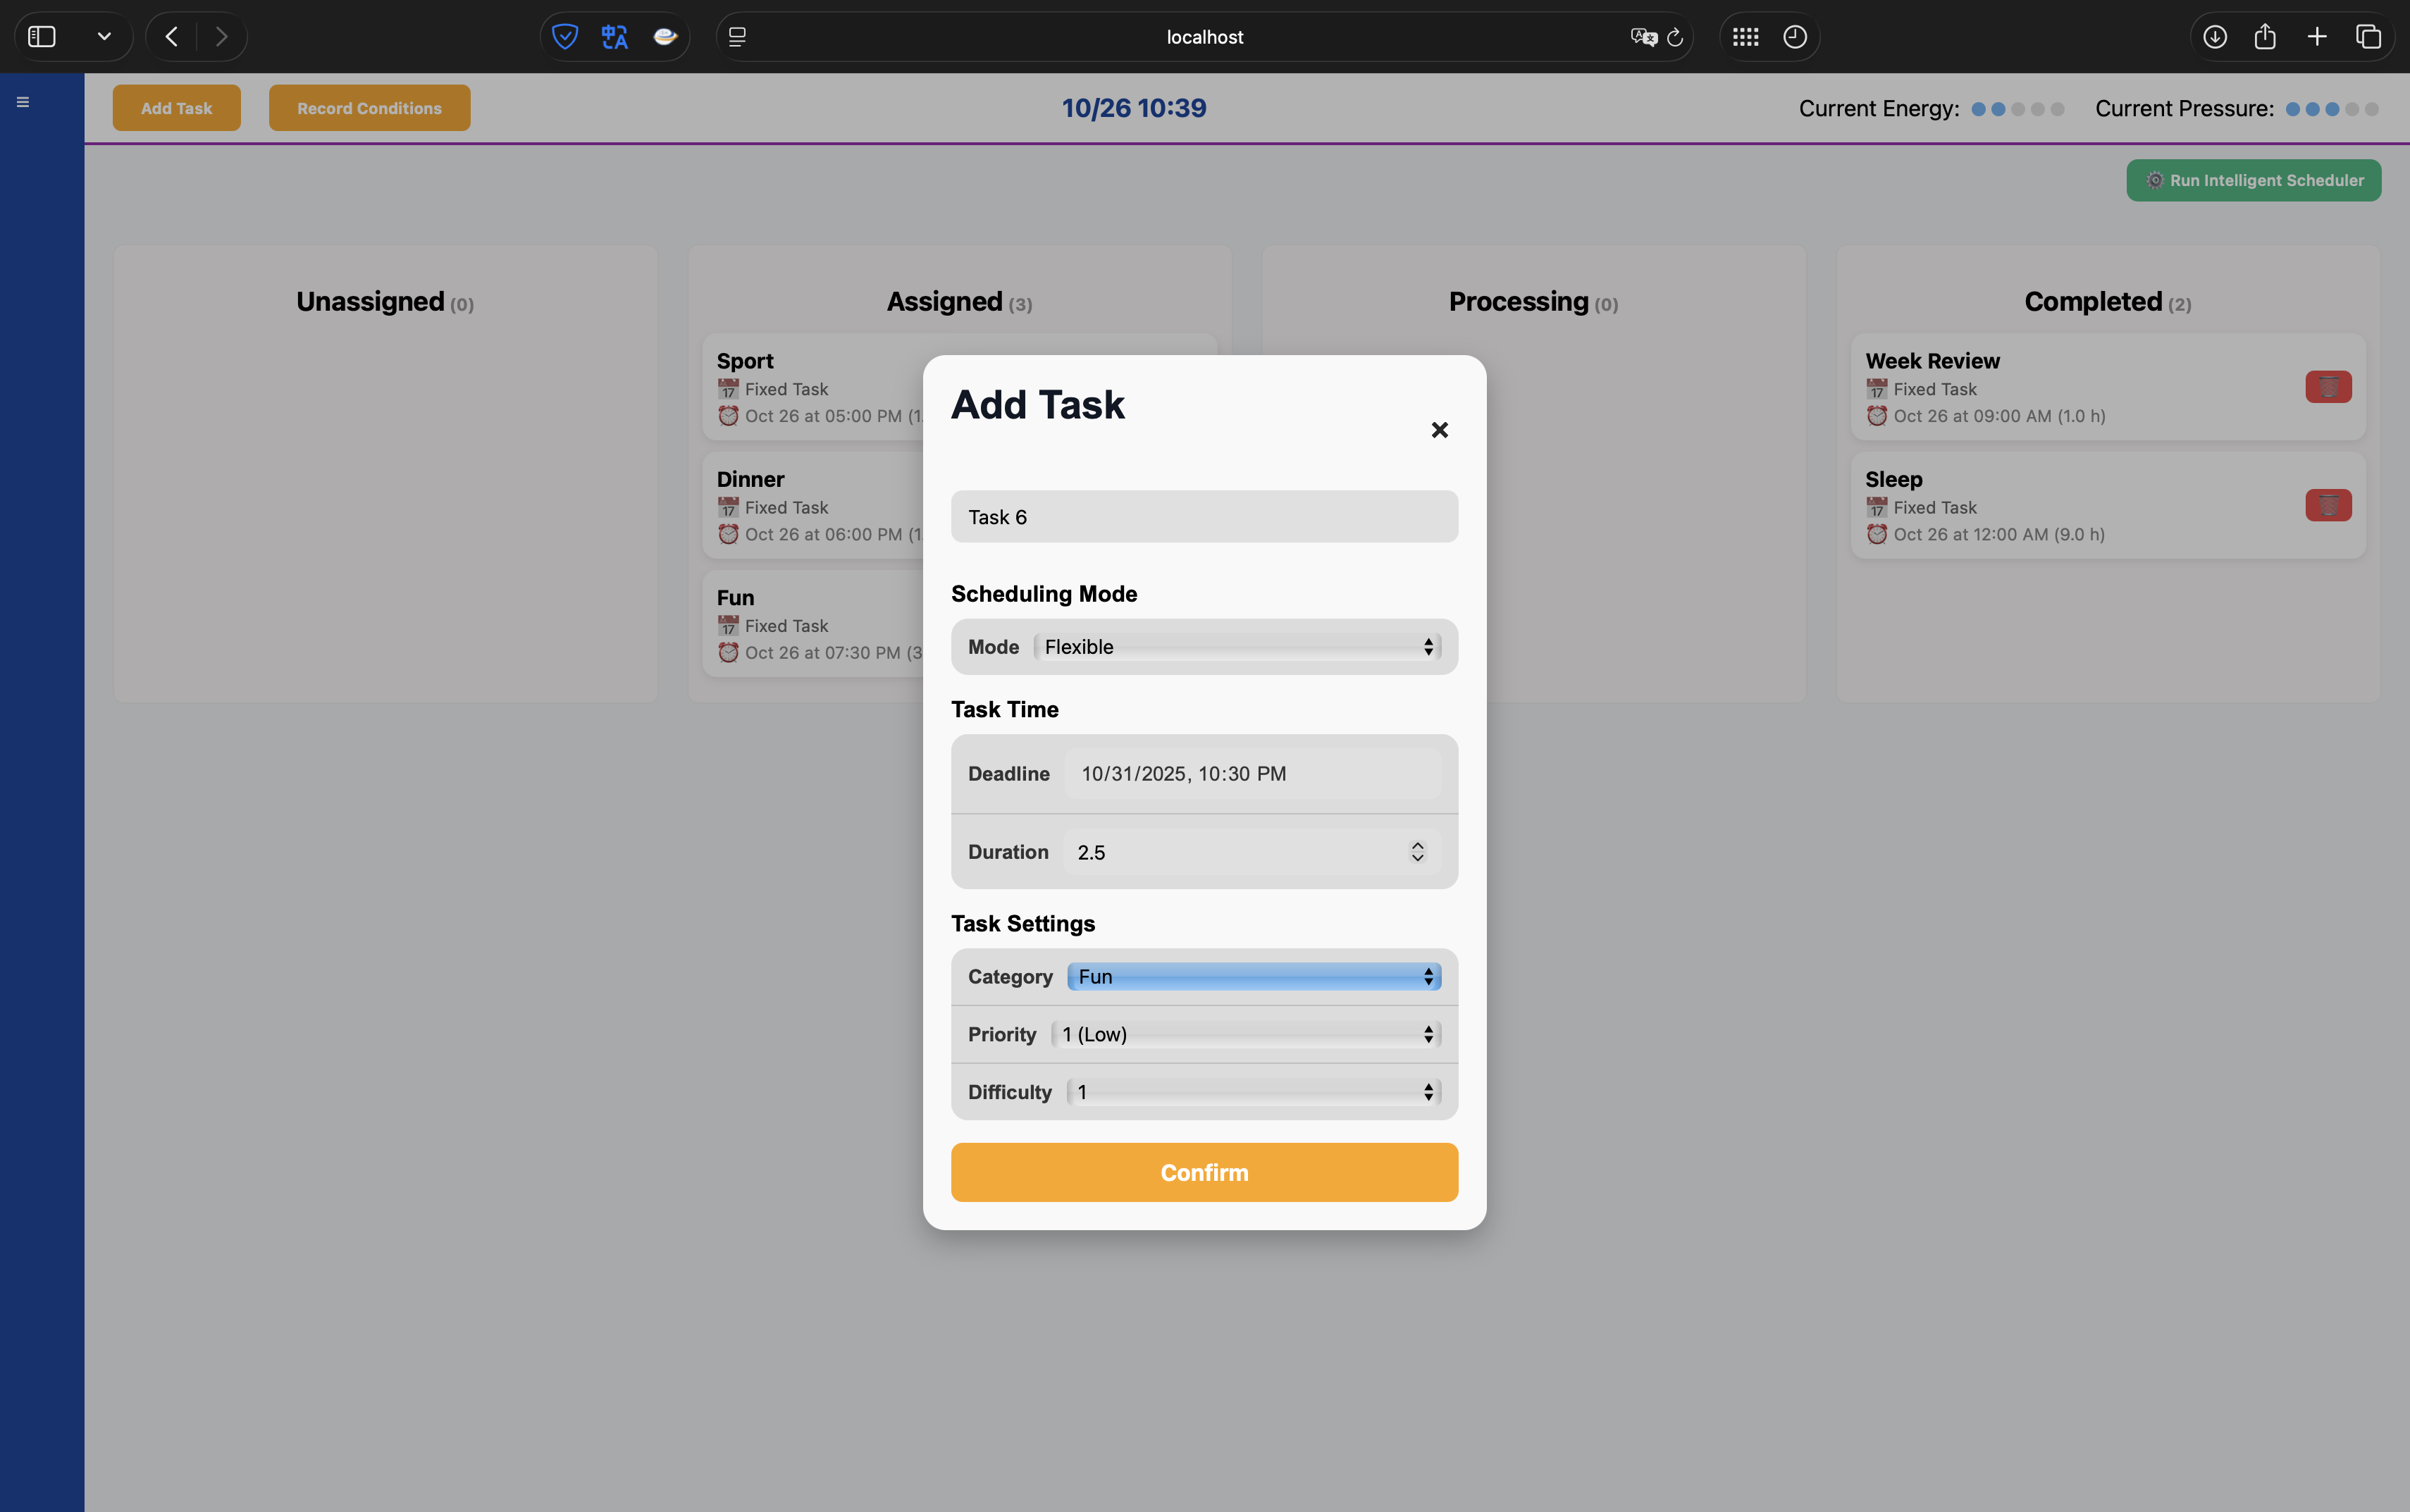
\includegraphics[width=\textwidth]{Images/System/ai_scheduling/add_flex.png}
                        \caption{Add Flexible Tasks}
                        \label{add_flex}
                    \end{figure}

                    \begin{figure}[H]
                        \begin{minipage}[t]{0.49\textwidth}
                            \centering
                            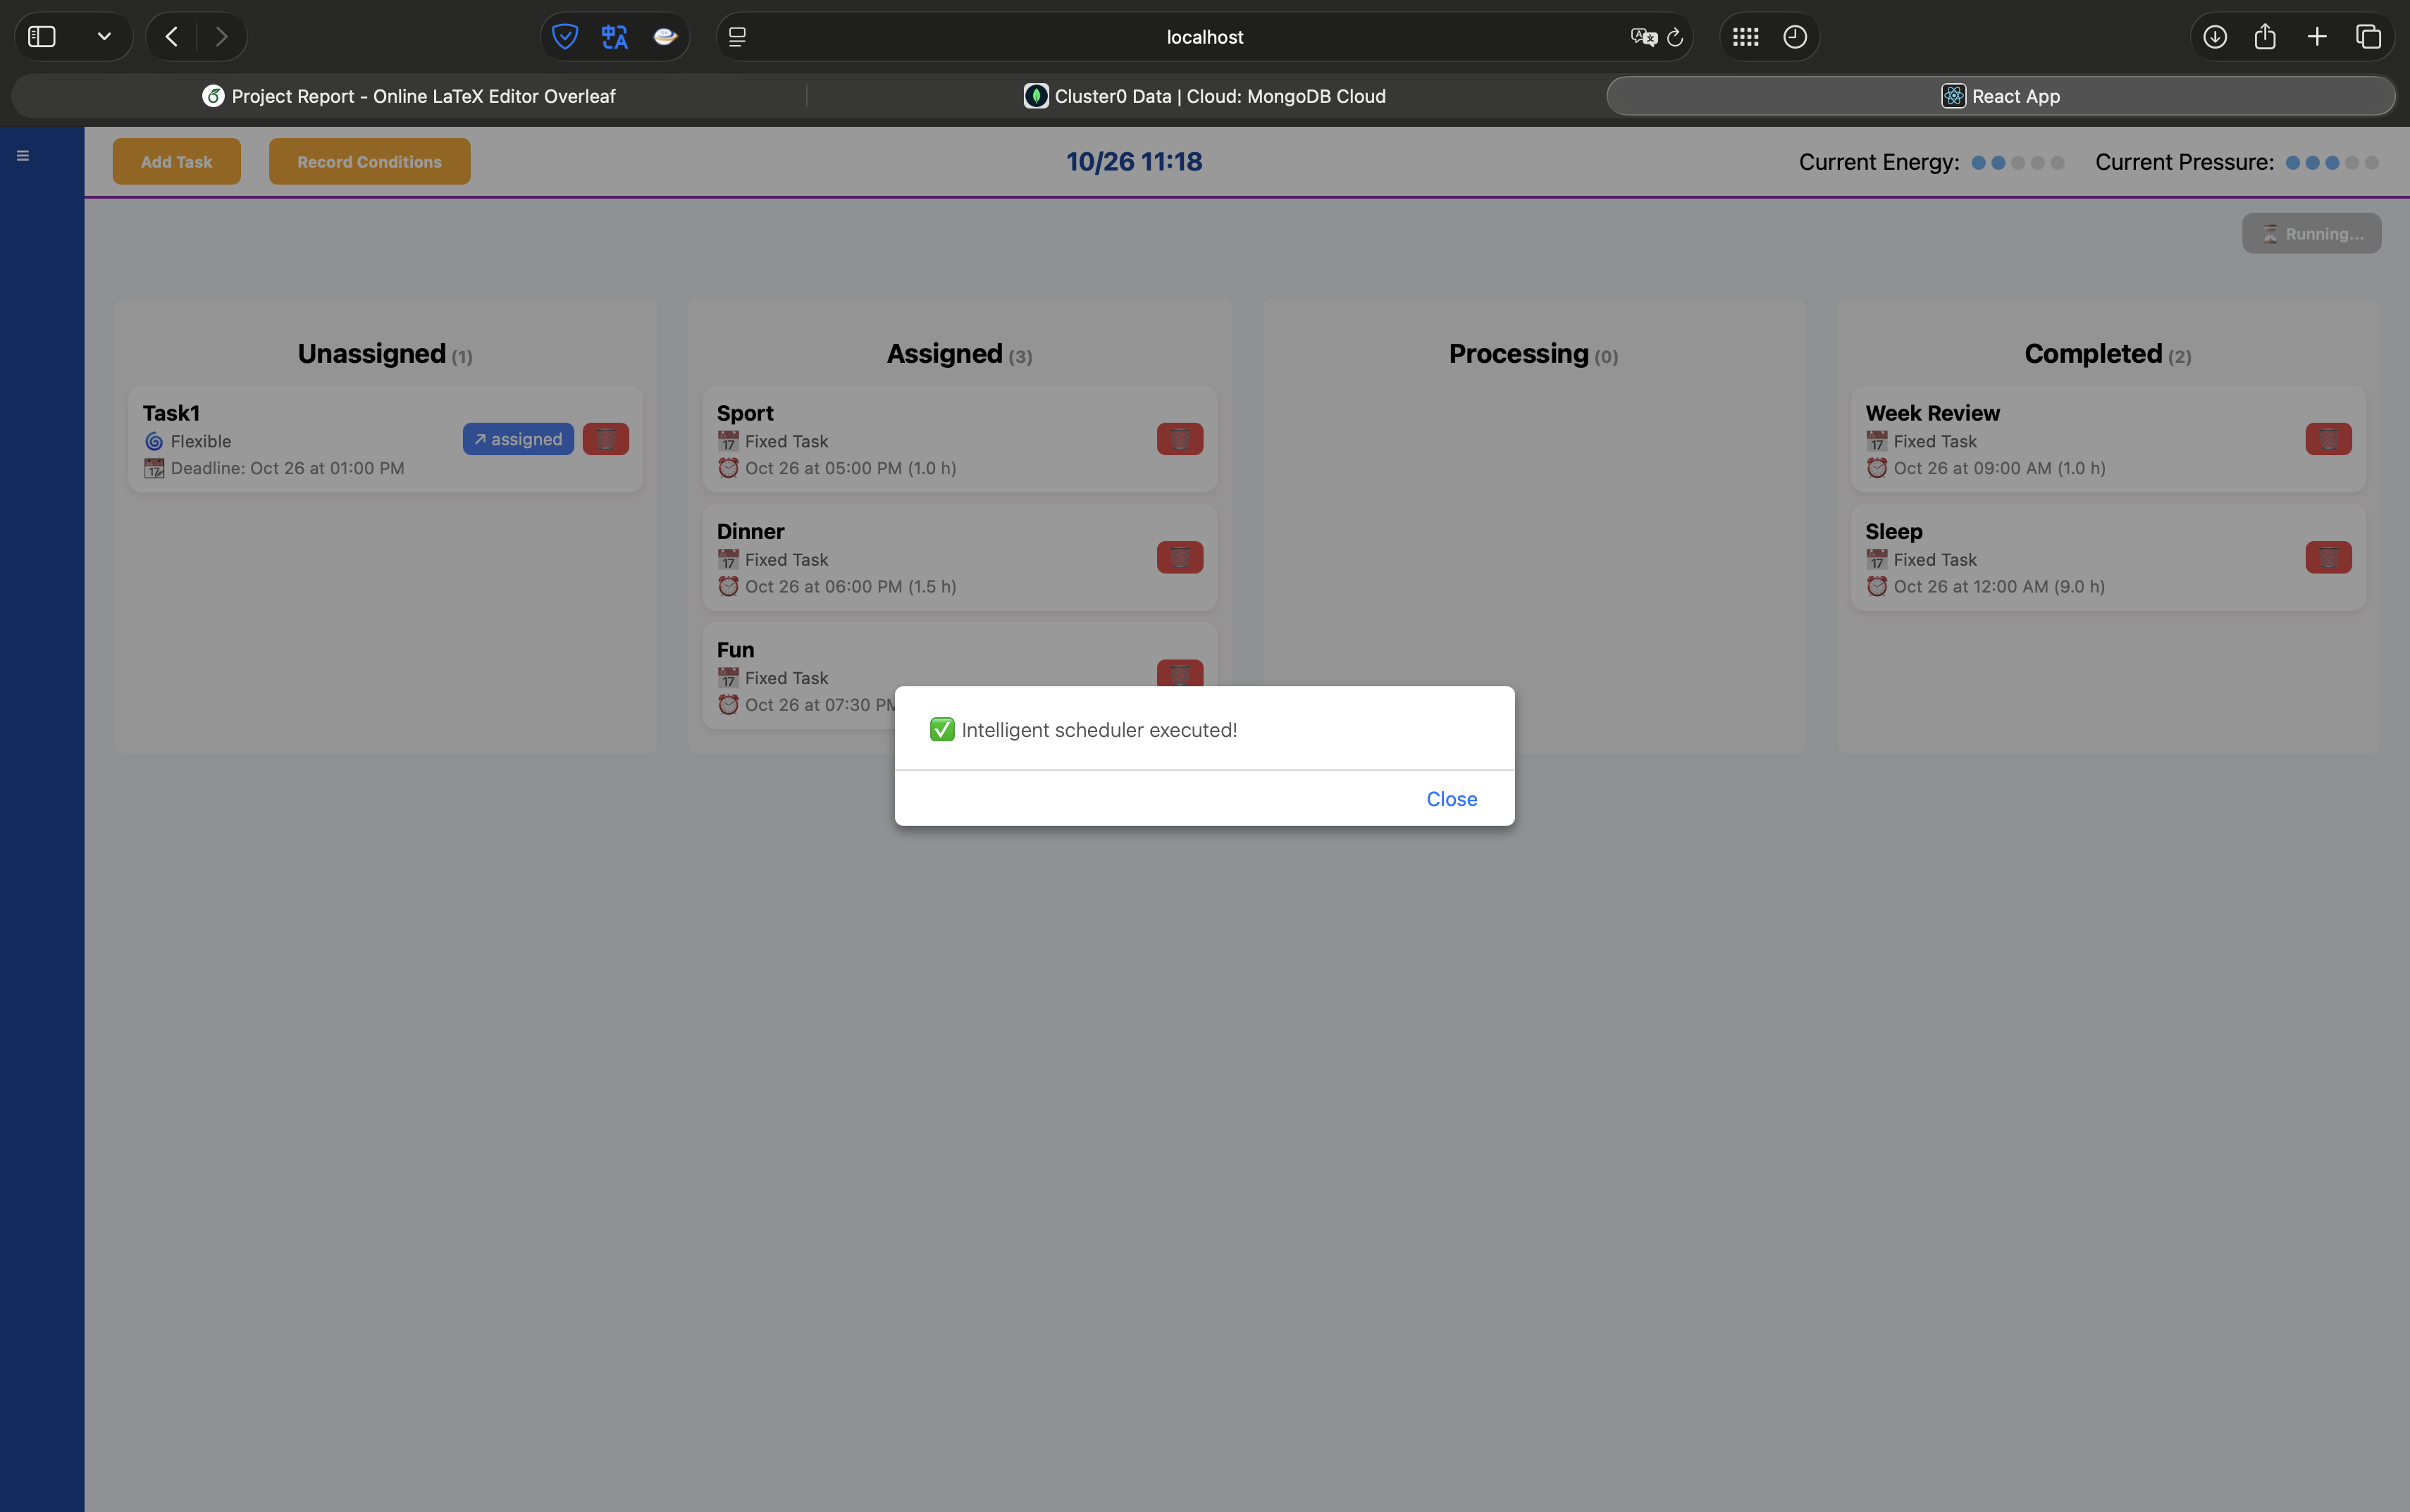
\includegraphics[width=\textwidth]{Images/System/ai_scheduling/sch_succ.png}
                            \caption{Prompt - Scheduling Succeed! }
                            \label{sch_succ}
                        \end{minipage}
                        \hfill
                        \begin{minipage}[t]{0.49\textwidth}
                            \centering
                            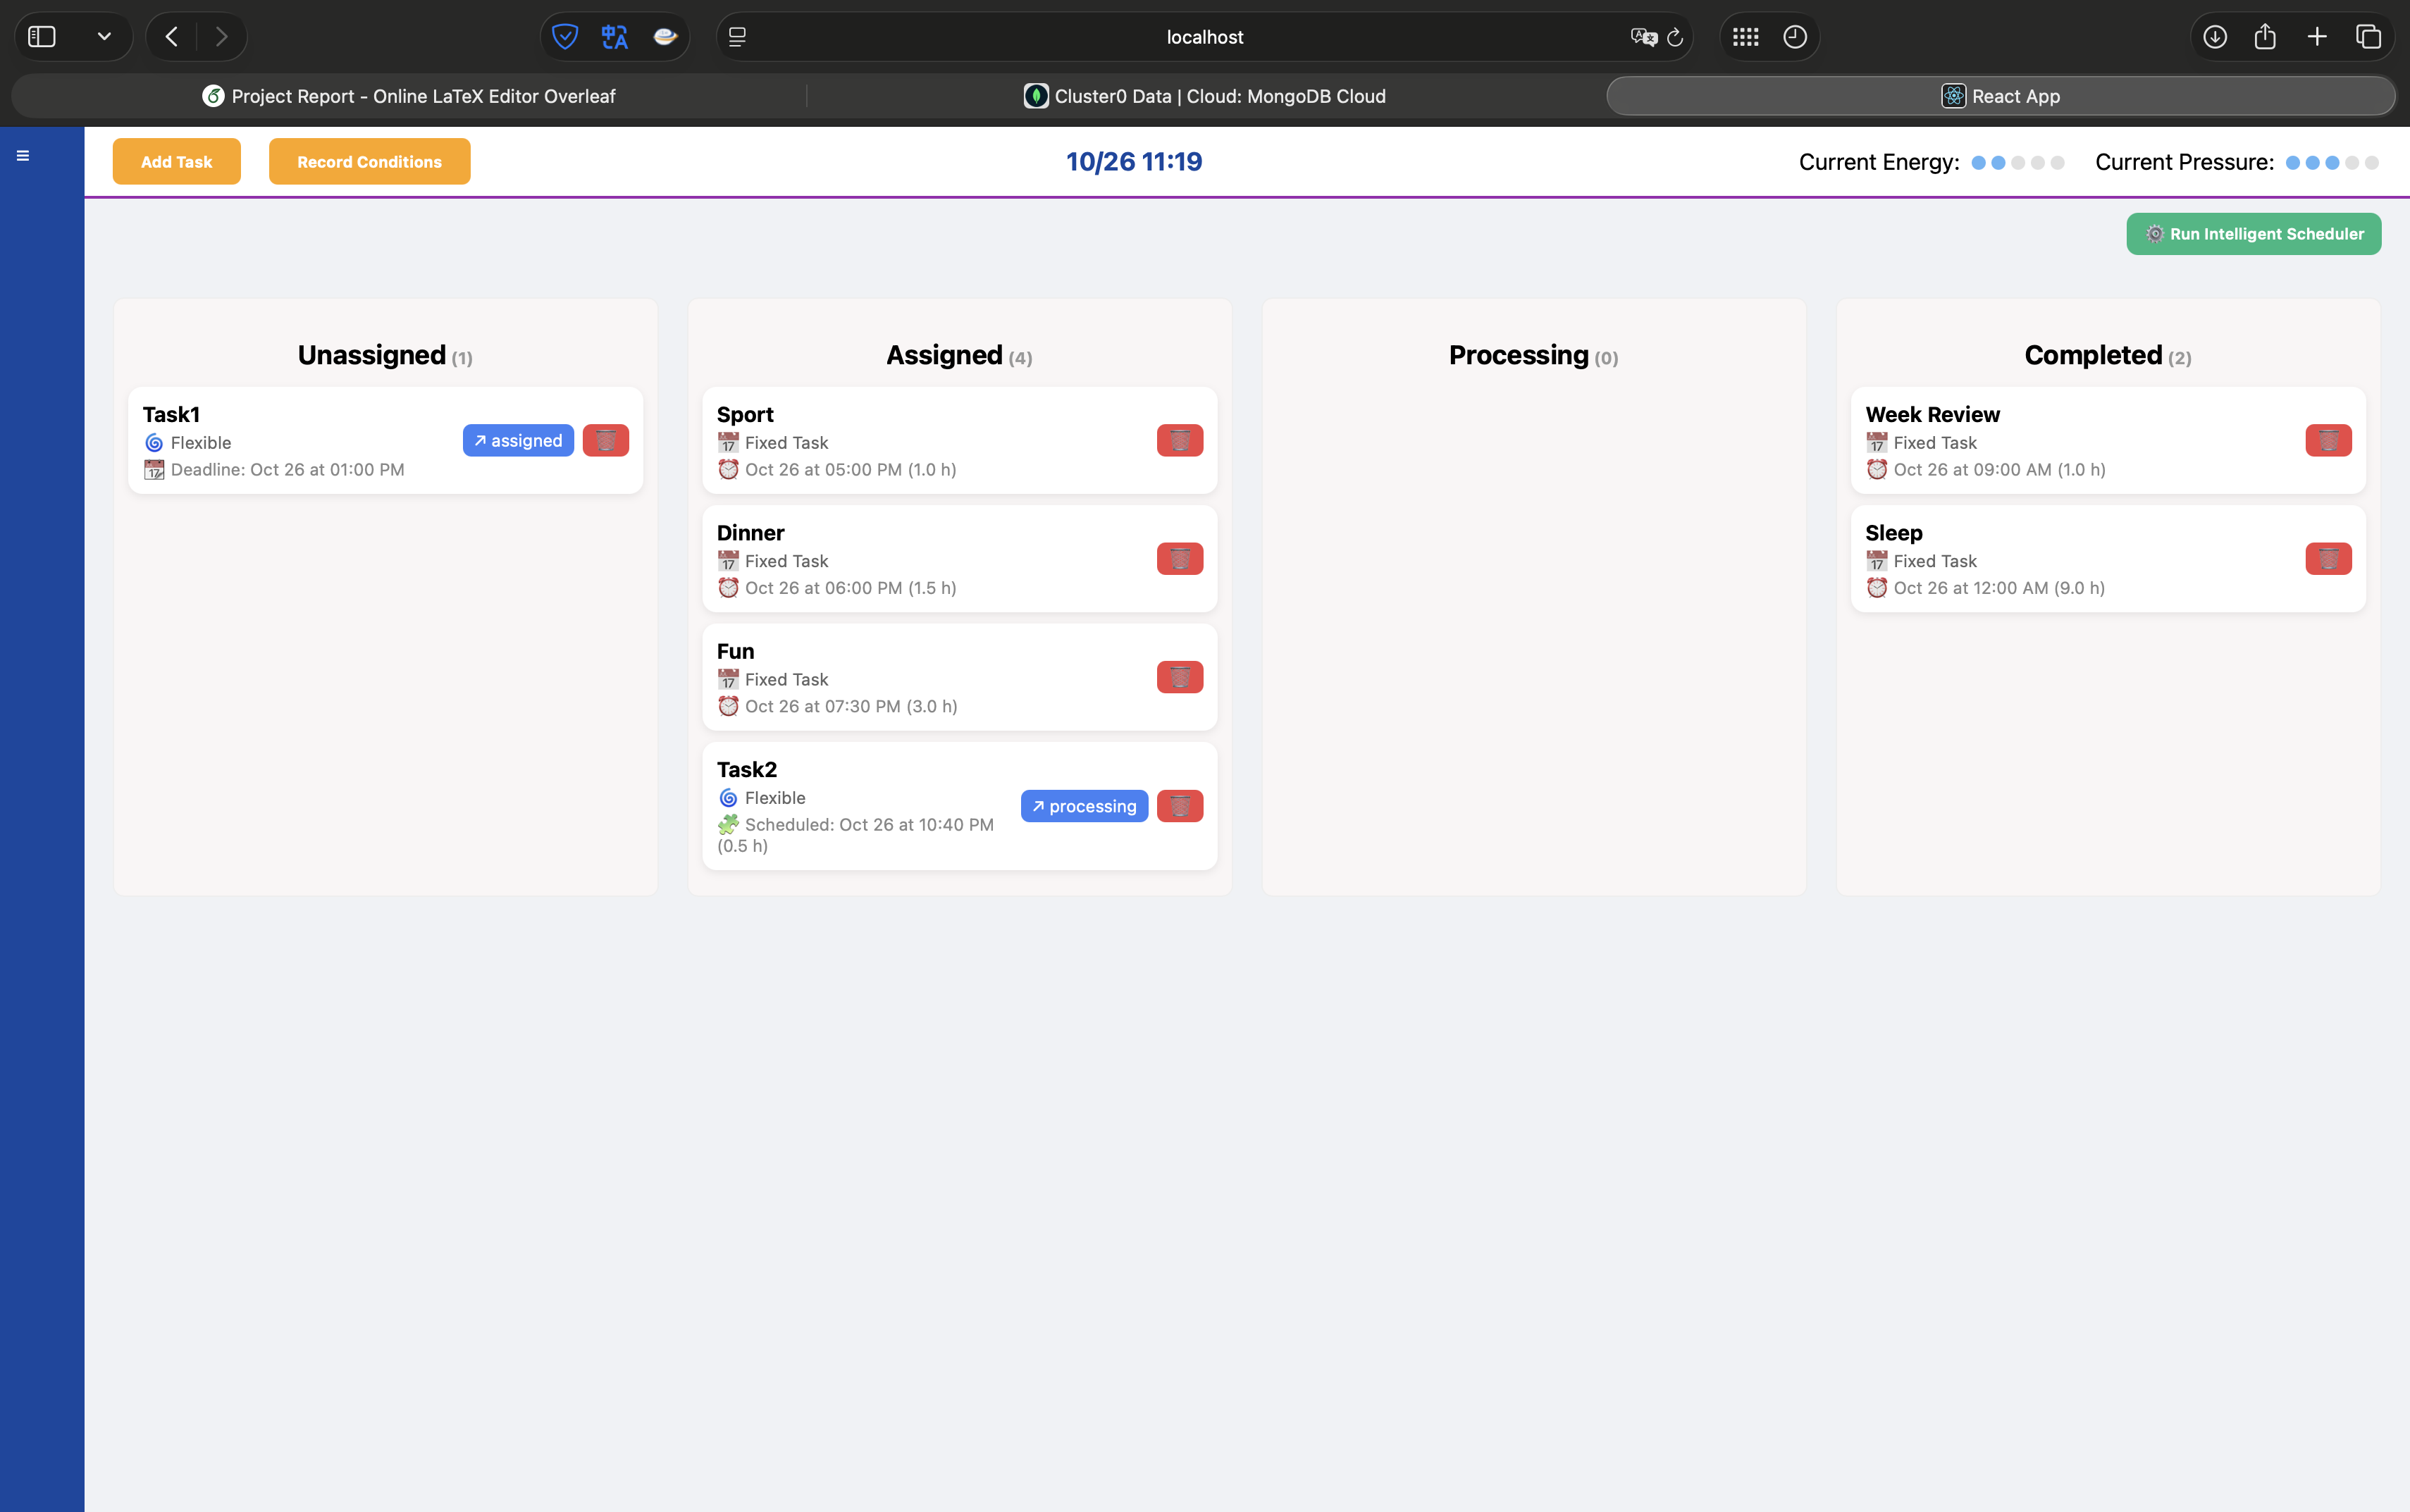
\includegraphics[width=\textwidth]{Images/System/ai_scheduling/aft_sch_todaytask.png}
                            \caption{Today Tasks after AI-Scheduling}
                            \label{aft_sch_todaytask}
                        \end{minipage}
                    \end{figure}

                    \begin{figure}[H]
                        \begin{minipage}[t]{0.49\textwidth}
                            \centering
                            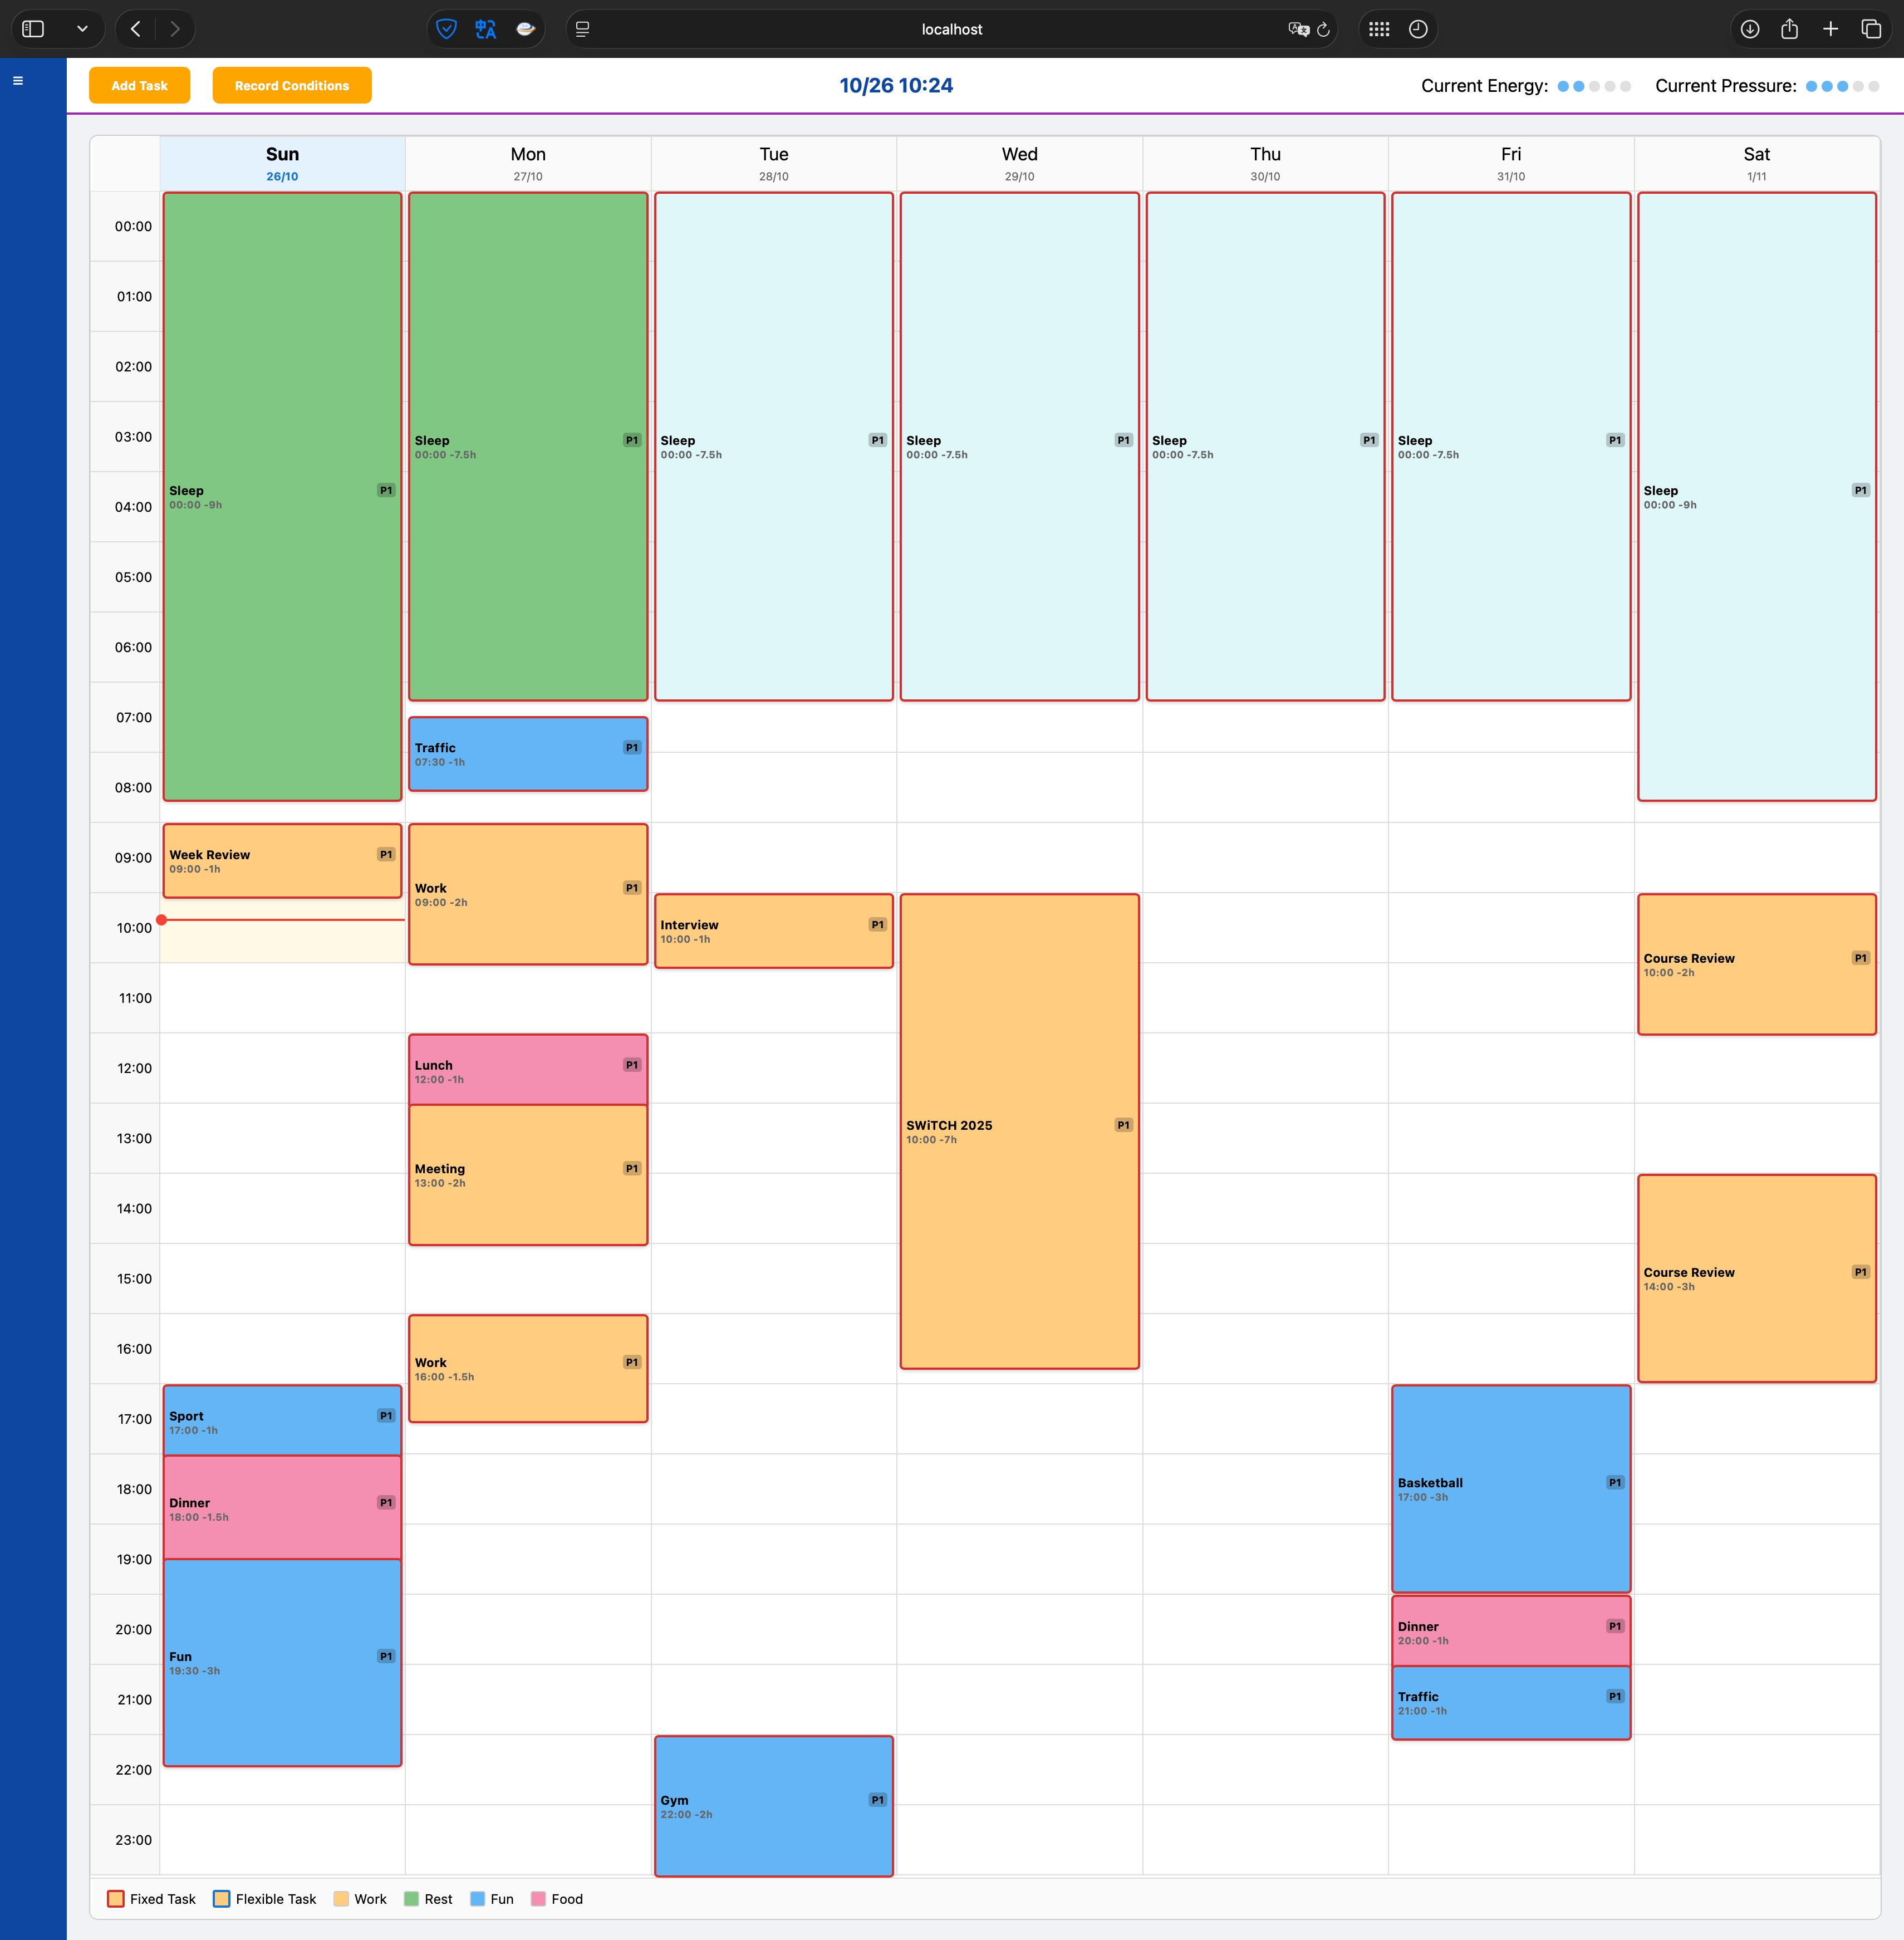
\includegraphics[width=\textwidth]{Images/System/ai_scheduling/bf_scheduling.JPG}
                            \caption{Timetable before AI-Scheduling}
                            \label{bf_scheduling}
                        \end{minipage}
                        \hfill
                        \begin{minipage}[t]{0.49\textwidth}
                            \centering
                            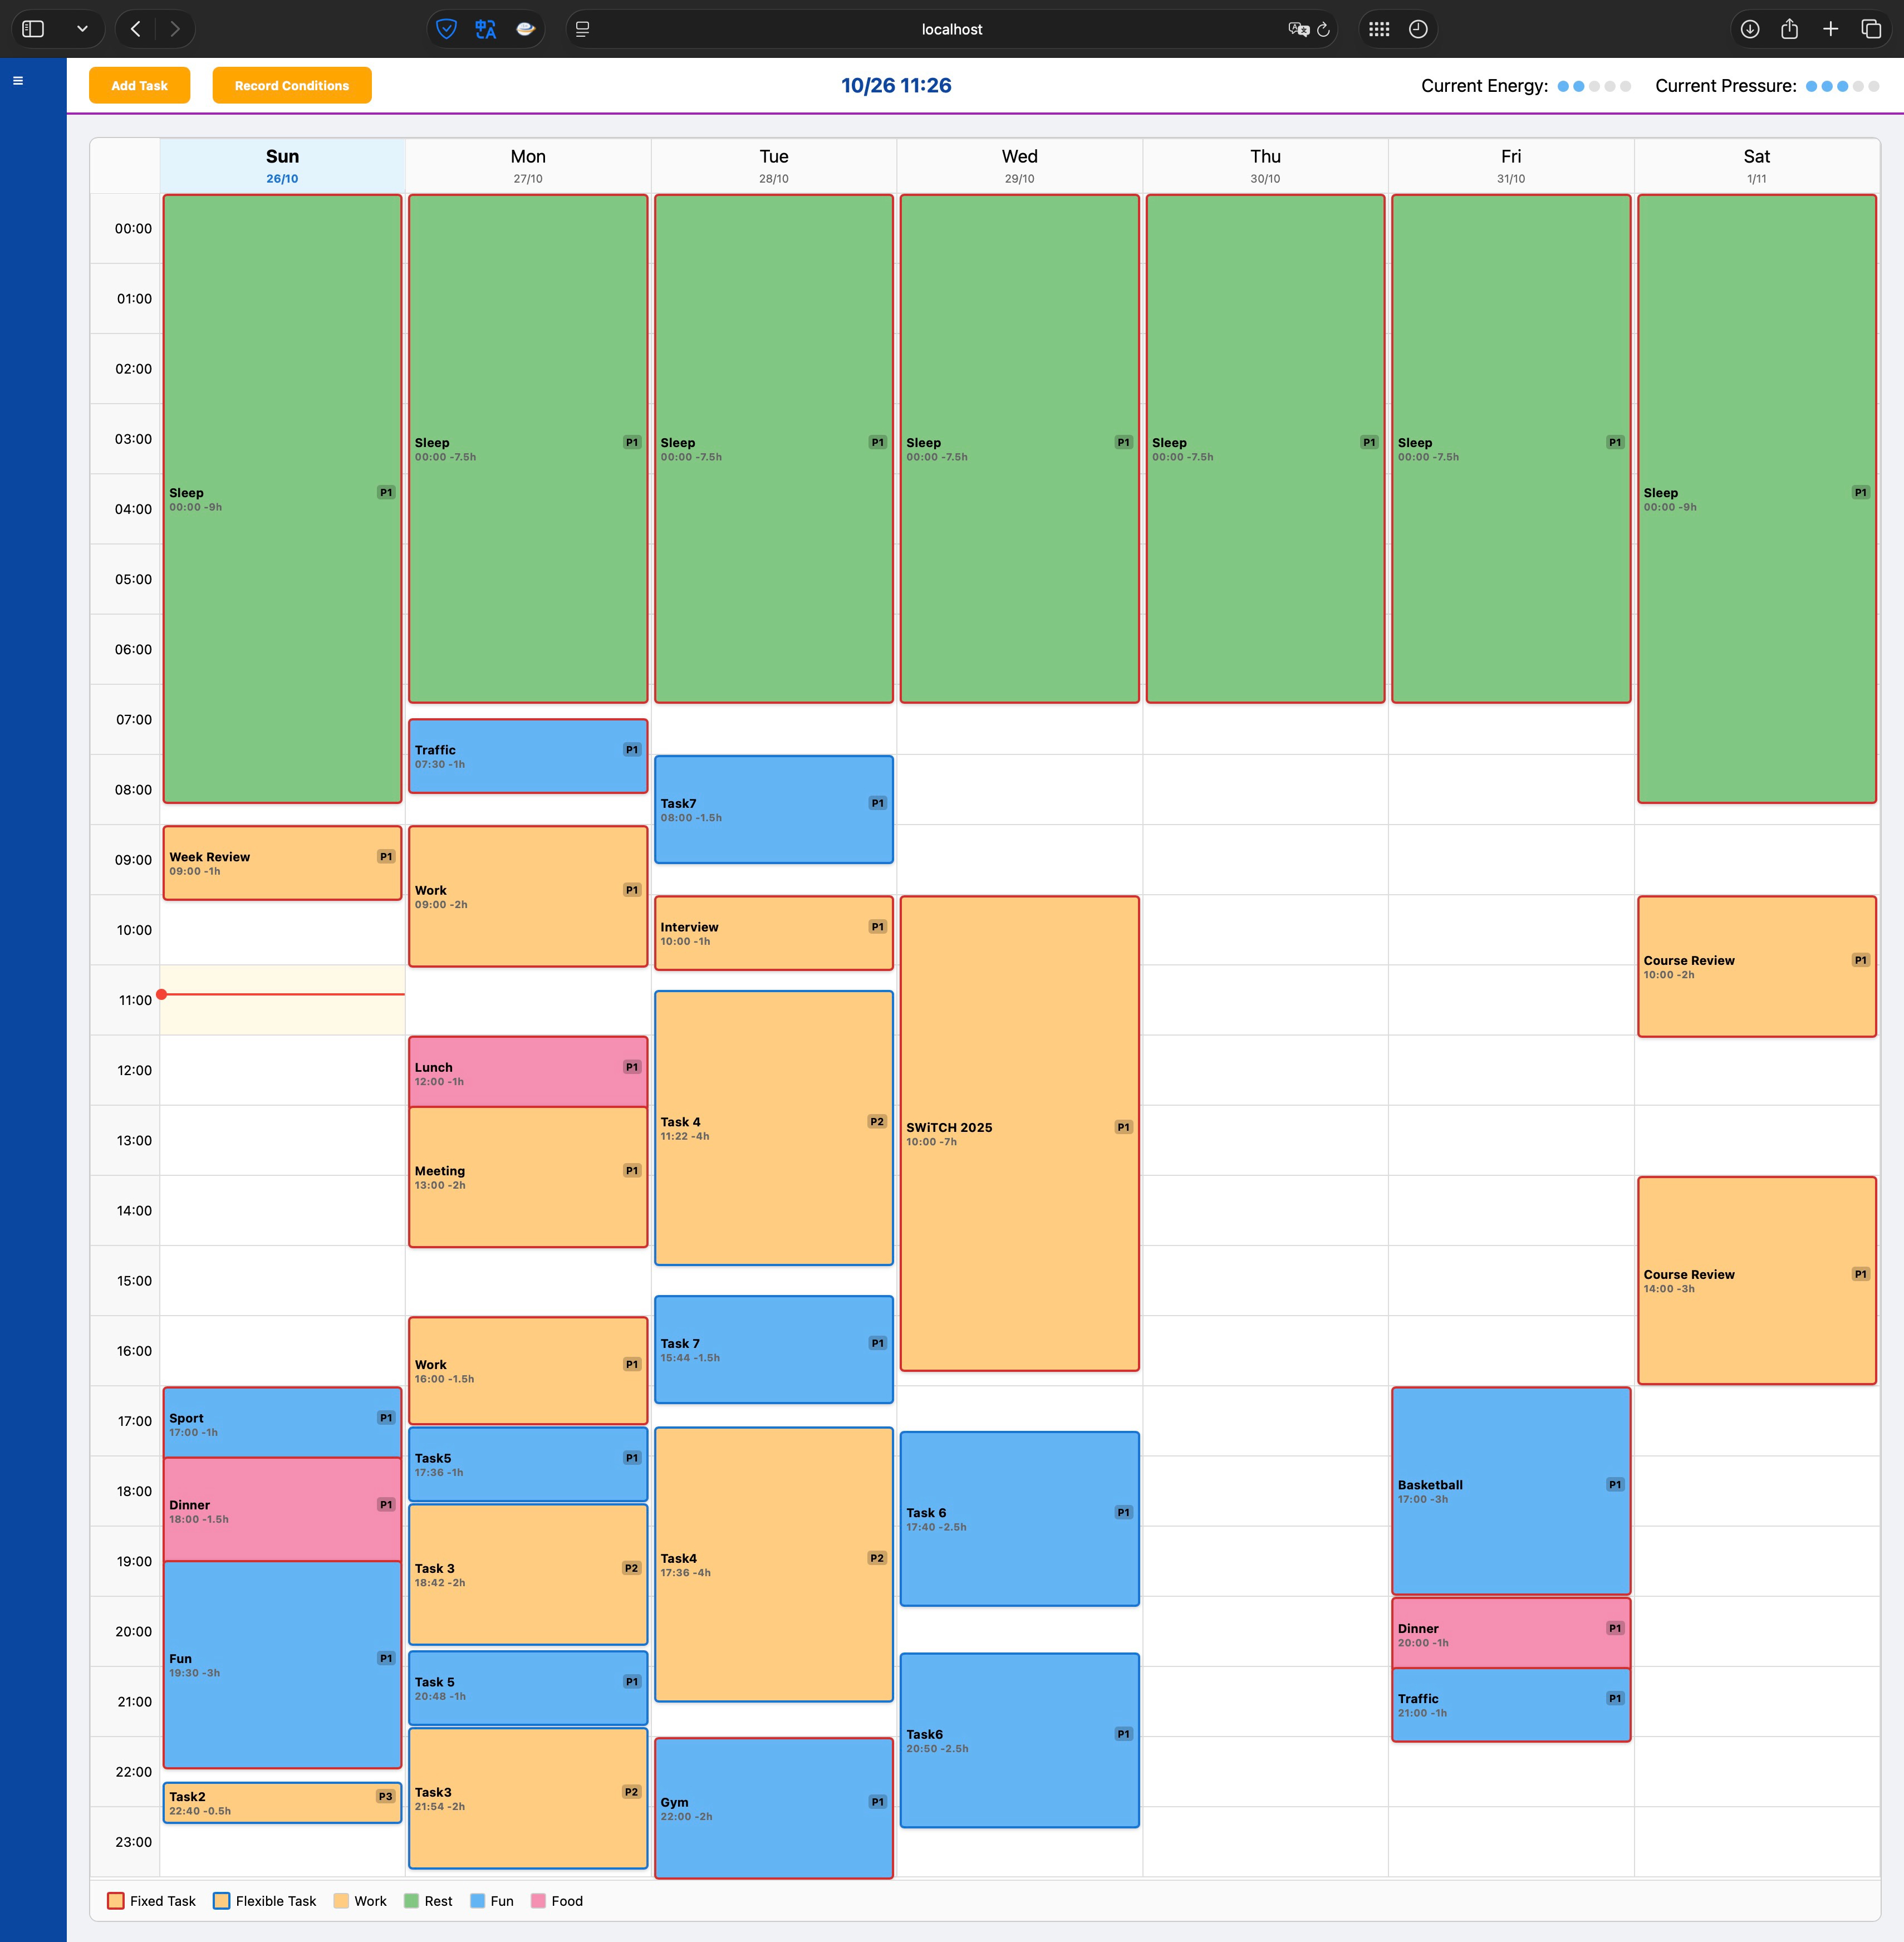
\includegraphics[width=\textwidth]{Images/System/ai_scheduling/aft_scheduling.jpeg}
                            \caption{Timetable after AI-Scheduling}
                            \label{aft_scheduling}
                        \end{minipage}
                    \end{figure}

                \item \textbf{Intelligent Report}
                                
                    The \textbf{Intelligent Report} module provides an analytical visualization of the user’s daily and weekly performance, bridging the reasoning engine with interpretable insights. It is designed not only to display completed tasks and statistics but also to reflect patterns in user behavior, energy consumption, and psychological pressure trends over time. By combining data analytics and adaptive visualization, this component transforms raw scheduling data into actionable self-awareness. 
    
                    \begin{itemize}
                        \item \textbf{Daily Report}
    
                            As shown in Figure~\ref{daily_report}, the daily report panel presents an overview of the user's performance on a specific day. It consists of three main sections:
                        
                            \begin{enumerate}
                                \item \textbf{Task Status Summary}: Displays total number of tasks, number of completed ones, and the completion rate. This section offers a quantitative reflection of user productivity.
                                \item \textbf{Task Type Distribution}: A pie chart categorizing tasks into work, food, rest and fun. This distribution helps the user identify whether their schedule maintains a healthy balance between professional and leisure activities.
                                \item \textbf{Energy \& Pressure Trends}: Line charts that visualize predicted energy and stress levels throughout the day. These curves are derived from the AI Task Evaluation Model, showing how task arrangement impacts the user’s well-being.
                            \end{enumerate}
            
                            \begin{figure}[H]
                                \centering
                                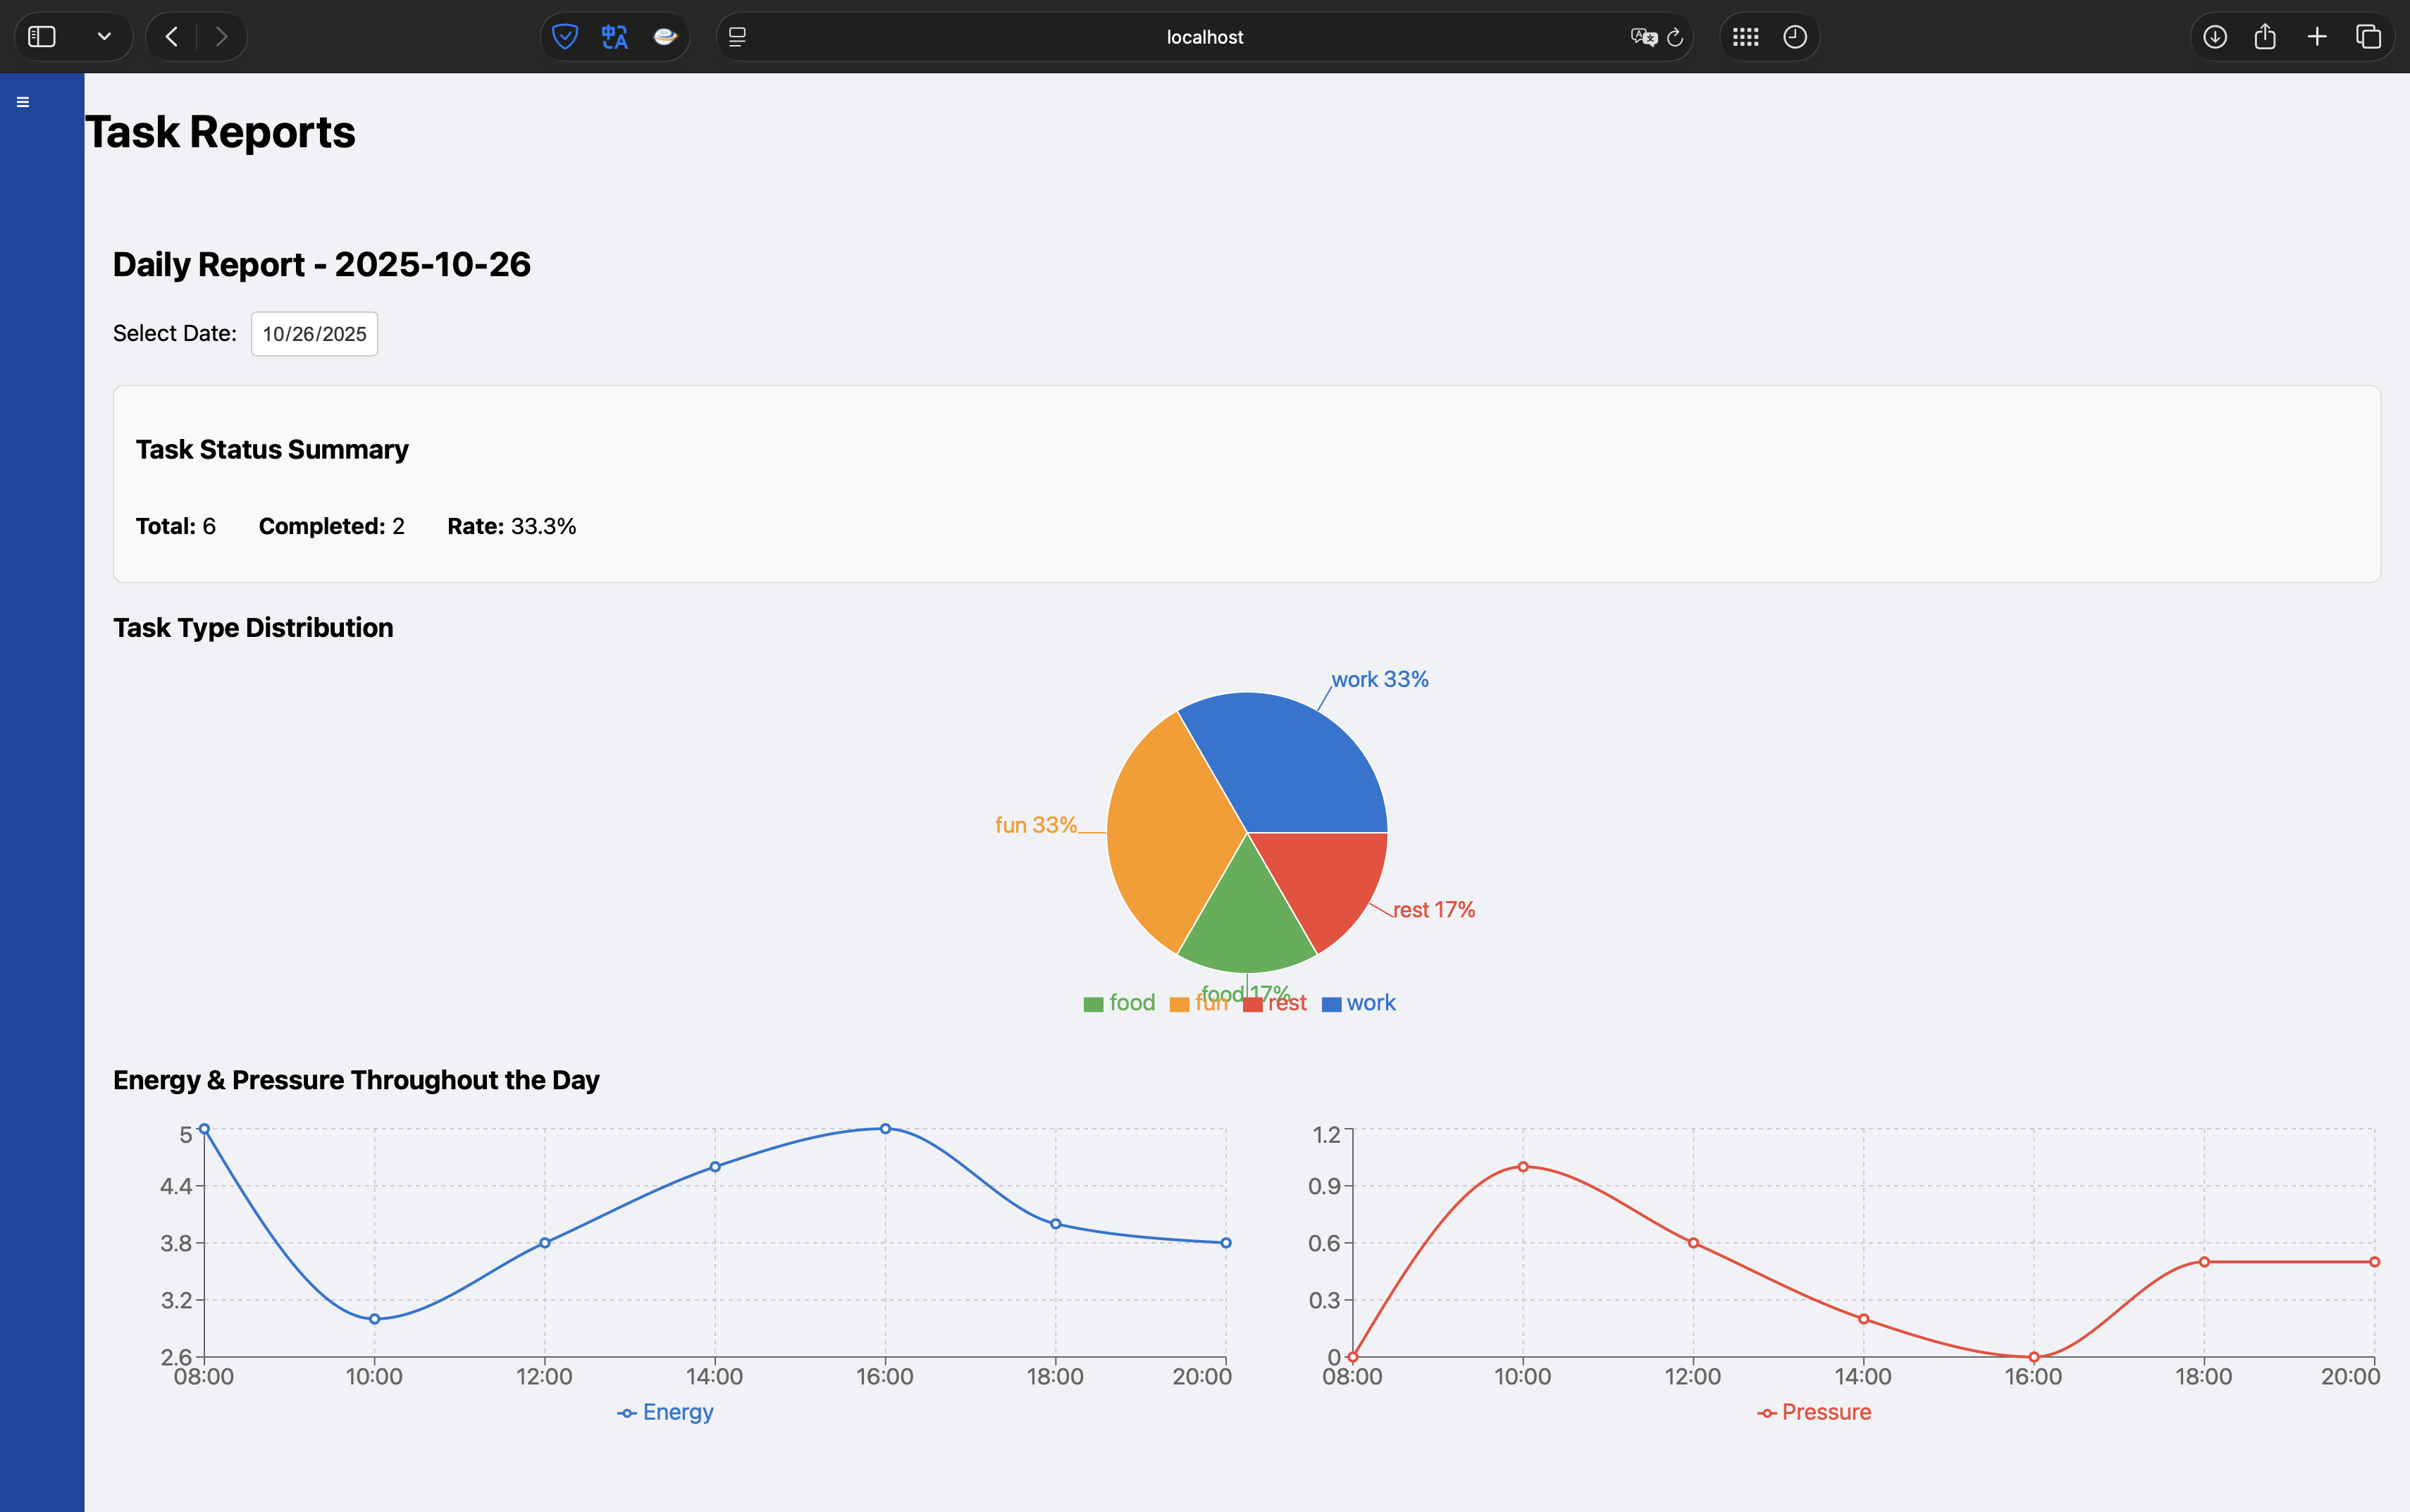
\includegraphics[width=\textwidth]{Images/System/report/daily_report.png}
                                \caption{Daily Report Interface}
                                \label{daily_report}
                            \end{figure}
    
                        \item \textbf{Weekly Report}
    
                            The weekly report (Figure~\ref{weekly_report1}) provides a longitudinal view of performance over seven days, summarizing total task counts, completion ratios, and changes in energy-pressure patterns. Key features include:
                            
                            \begin{enumerate}
                                \item \textbf{Weekly Summary}: Summarizes the total number of tasks and completion rate across the week.
                                \item \textbf{Daily Task Count}: A bar chart comparing total tasks per day, revealing workload fluctuations and potential over-scheduling days.
                                \item \textbf{Task Type Distribution}: Visualizes proportions of different task types (work, food, fun and rest), indicating the overall lifestyle balance across the week.
                                \item \textbf{Energy \& Pressure Trends}: Plots average energy and stress over the week, highlighting days with excessive fatigue or pressure peaks.
                            \end{enumerate}
                            
                            \begin{figure}[H]
                                \centering
                                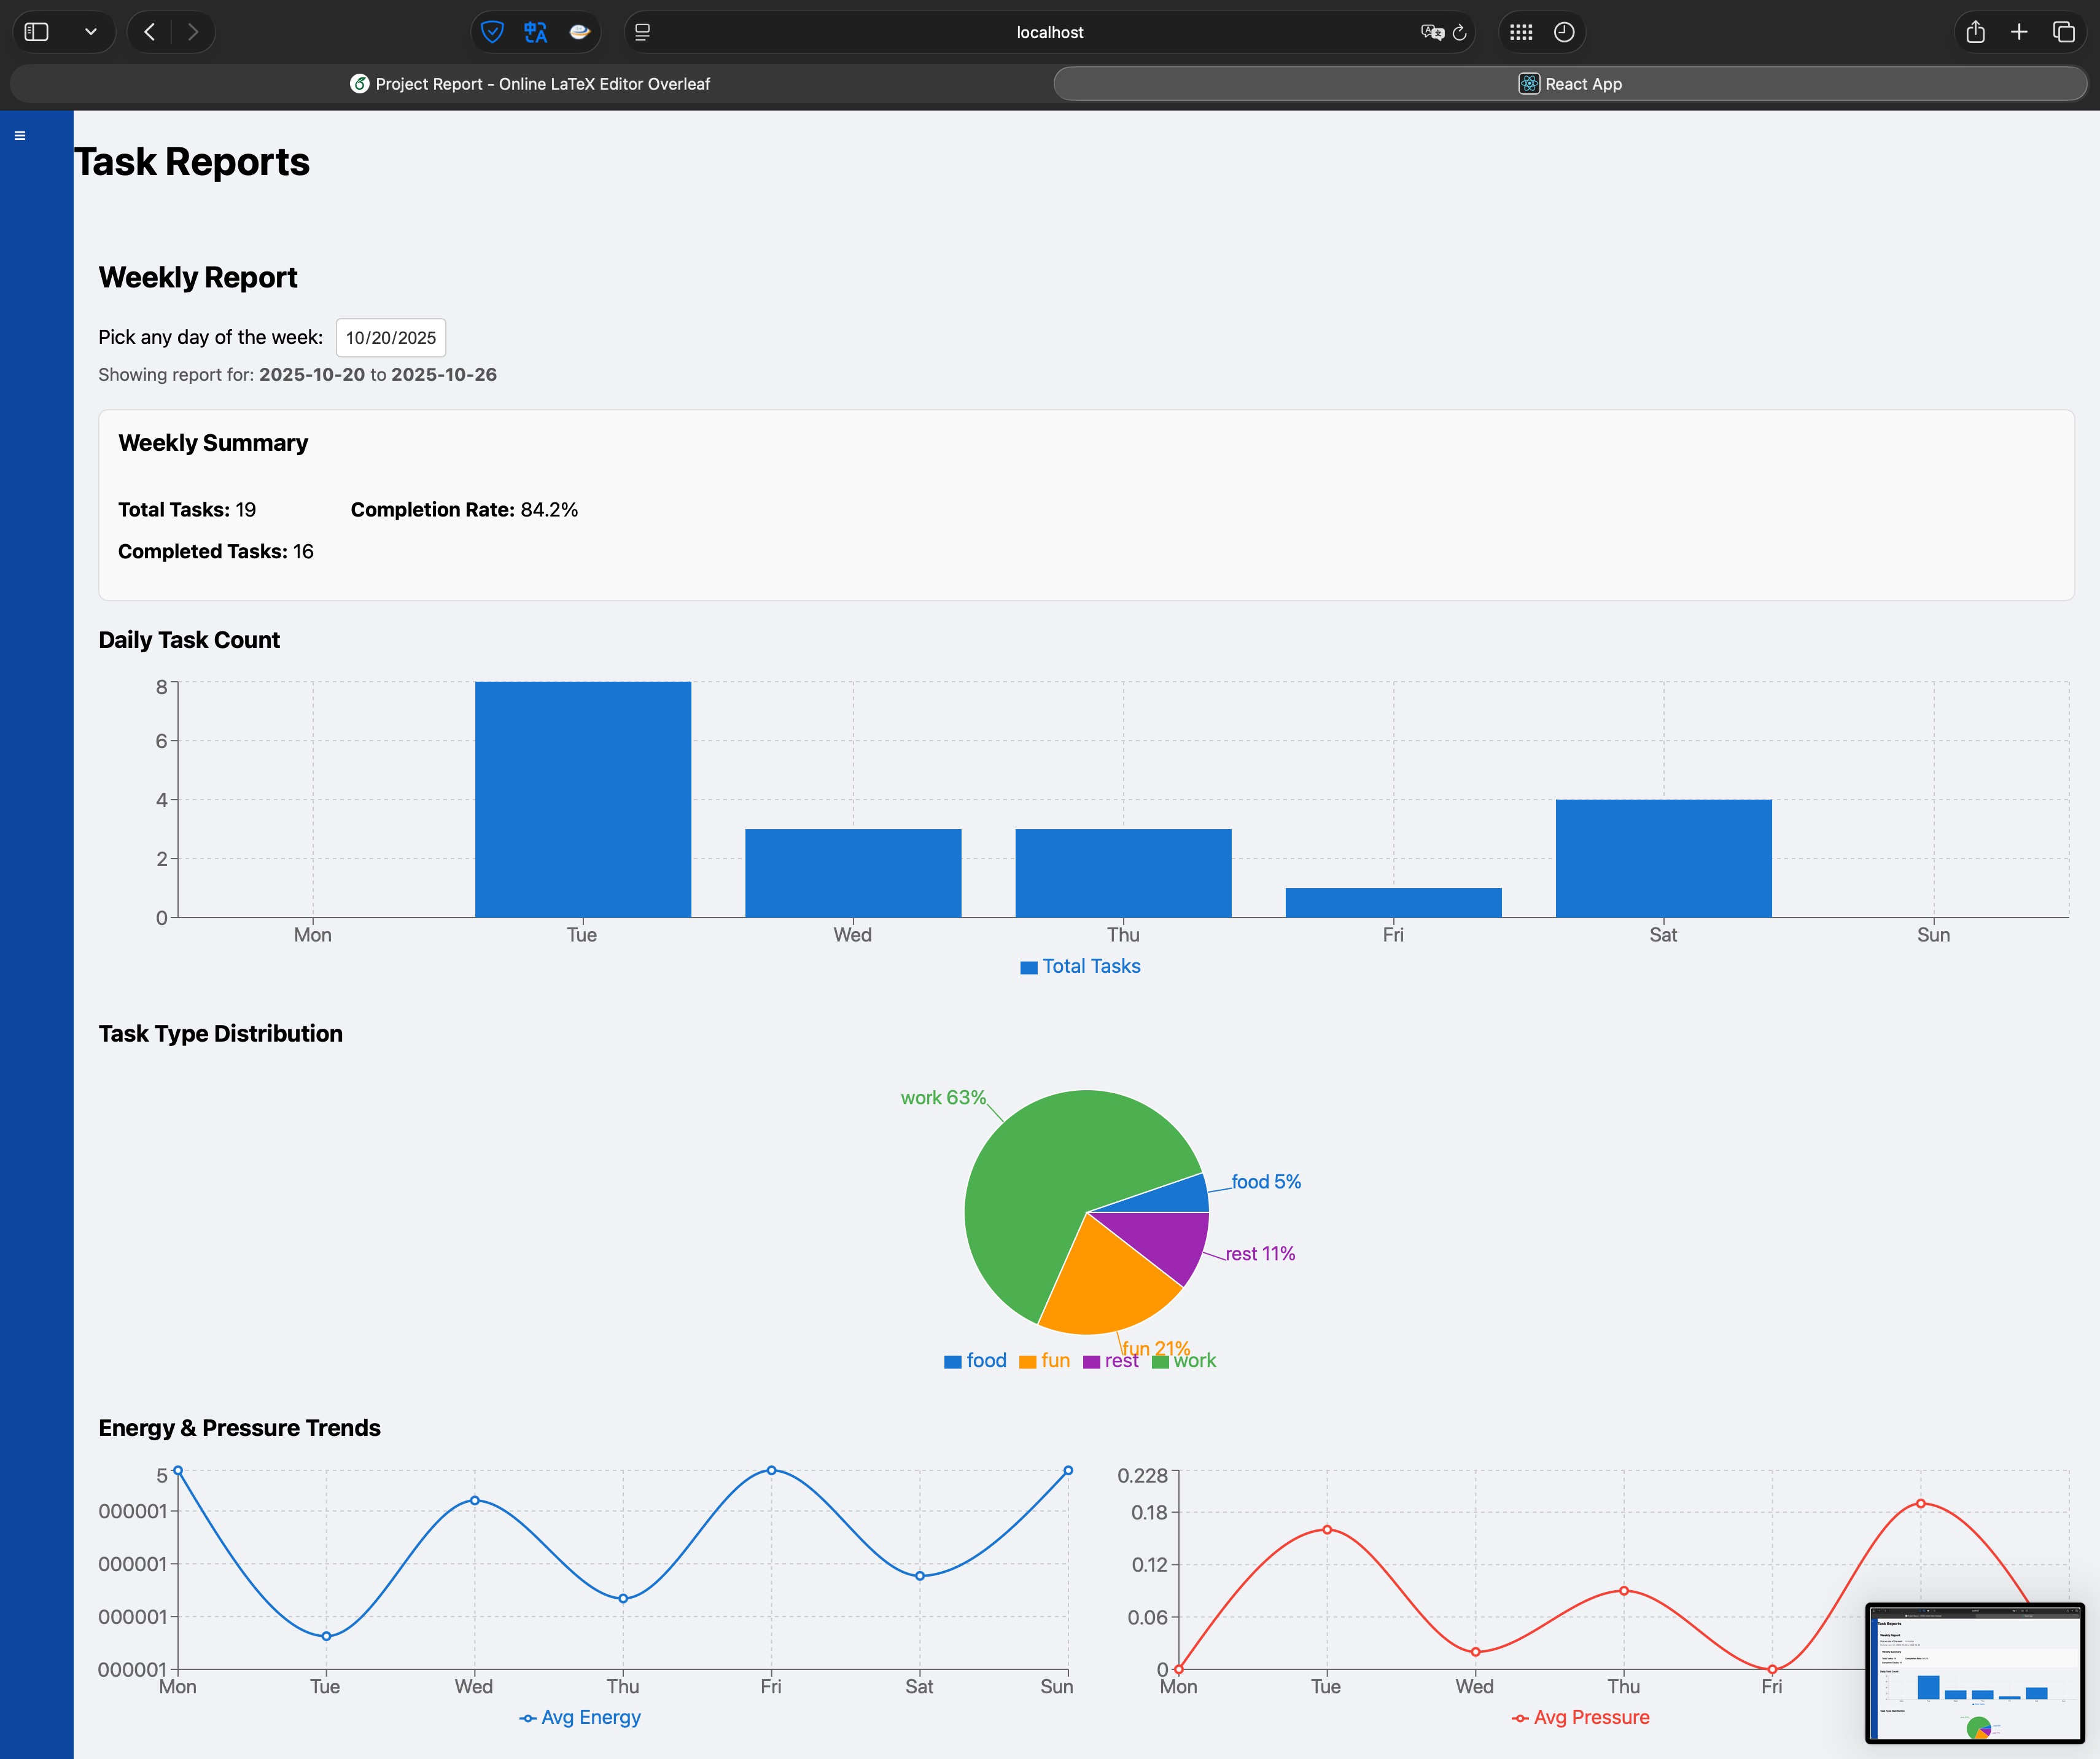
\includegraphics[width=\textwidth]{Images/System/report/weekly_report.JPG}
                                \caption{Weekly Report Overview}
                                \label{weekly_report1}
                            \end{figure}
    
                        \item \textbf{Analytical Insights.}  
                        
                            By combining daily and weekly reports, users can understand:
                            
                            \begin{enumerate}
                                \item \textbf{Productivity Patterns}: How the total workload and completion efficiency evolve over time.
                                \item \textbf{Lifestyle Balance}: Whether “work” tasks dominate excessively or leisure activities are underrepresented.
                                \item \textbf{Well-being Trends}: How energy depletion and pressure accumulation fluctuate throughout the week.
                            \end{enumerate}
                            
                    \end{itemize}
                    
                    These visualizations are dynamically generated based on real-time data queried from MongoDB and computed by the backend scheduler. They help users not only to reflect on past performance but also to adjust future schedules. The module demonstrates how AI-driven reasoning can be complemented by intuitive data visualization to support self-management, reflection, and long-term behavioral optimization.
                    
                                    
                \item \textbf{LLM Chatbot}
                
                    The \textbf{AI Task Chatbot} serves as a conversational interface that bridges natural language understanding and intelligent task automation. Instead of filling structured forms, users can directly describe their tasks in plain language, and the chatbot automatically interprets, structures, and adds them to the scheduling system. This component demonstrates the integration of Large Language Models (LLMs) with task reasoning, providing a natural, efficient, and human-centered interaction experience.

                    \begin{itemize}
                        \item \textbf{Natural Language Input}  

                            As shown in Figure~\ref{ai}, users can simply type a message such as:
                            
                            \begin{quote}
                                \textit{“Group meeting, 2025/10/25 at 10pm, 30 minutes, work.”}
                            \end{quote}
                            
                            The chatbot employs an embedded LLM to parse and extract structured task attributes, including:
                            
                            \begin{enumerate}
                                \item \textbf{Task name} (“group meeting”)
                                \item \textbf{Task mode} (fixed)
                                \item \textbf{Start time} (2025-10-25 22:00)
                                \item \textbf{Duration} (30 minutes)
                                \item \textbf{Task type} (work)
                            \end{enumerate}

                            If the LLM detects that the input explicitly includes a start time, the task is automatically categorized as a \textbf{fixed task}. Otherwise, when the description lacks a specific starting time, it is interpreted as a \textbf{flexible task} whose scheduling window will later be optimized by the system. 
                            
                            After determining the task mode, the chatbot performs entity extraction to identify all available attributes (time, duration, type, etc.) and prepares the structured task object for backend processing. 

                            \begin{figure}[H]
                                \centering
                                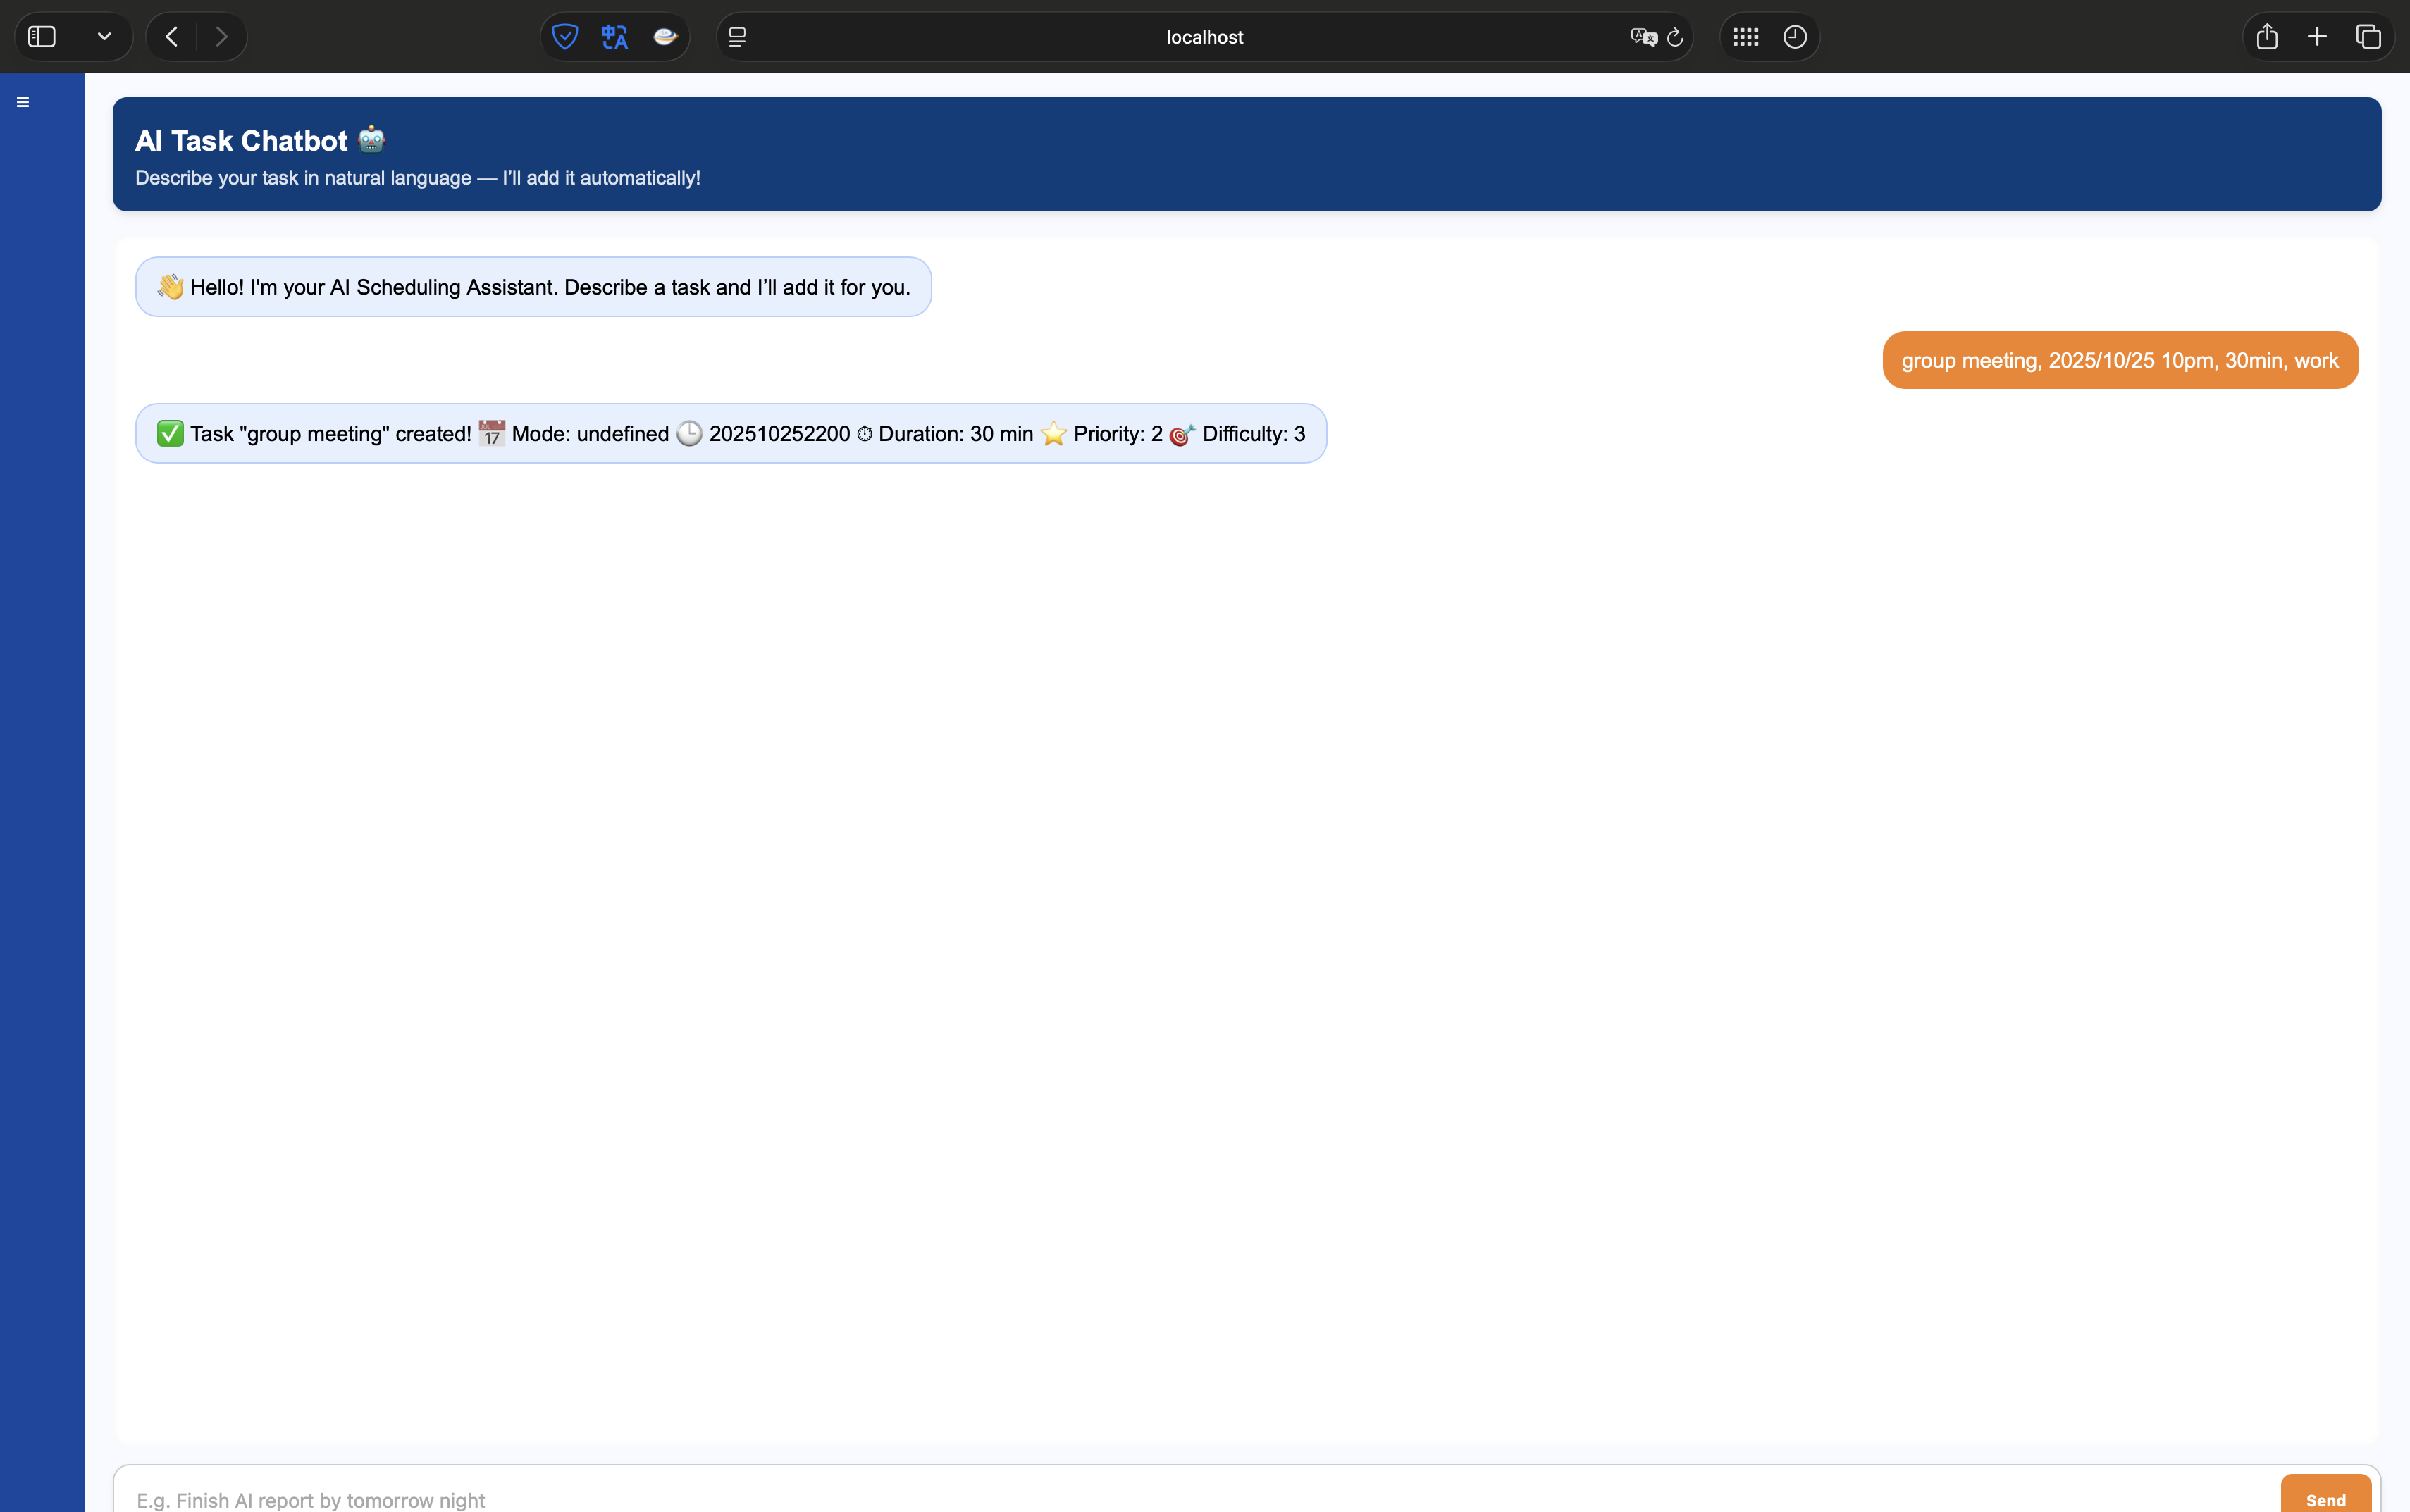
\includegraphics[width=\textwidth]{Images/System/chatbot/ai.png}
                                \caption{AI Chatbot}
                                \label{ai}
                            \end{figure}
        
                            \begin{figure}[H]
                                \begin{minipage}[t]{0.49\textwidth}
                                    \centering
                                    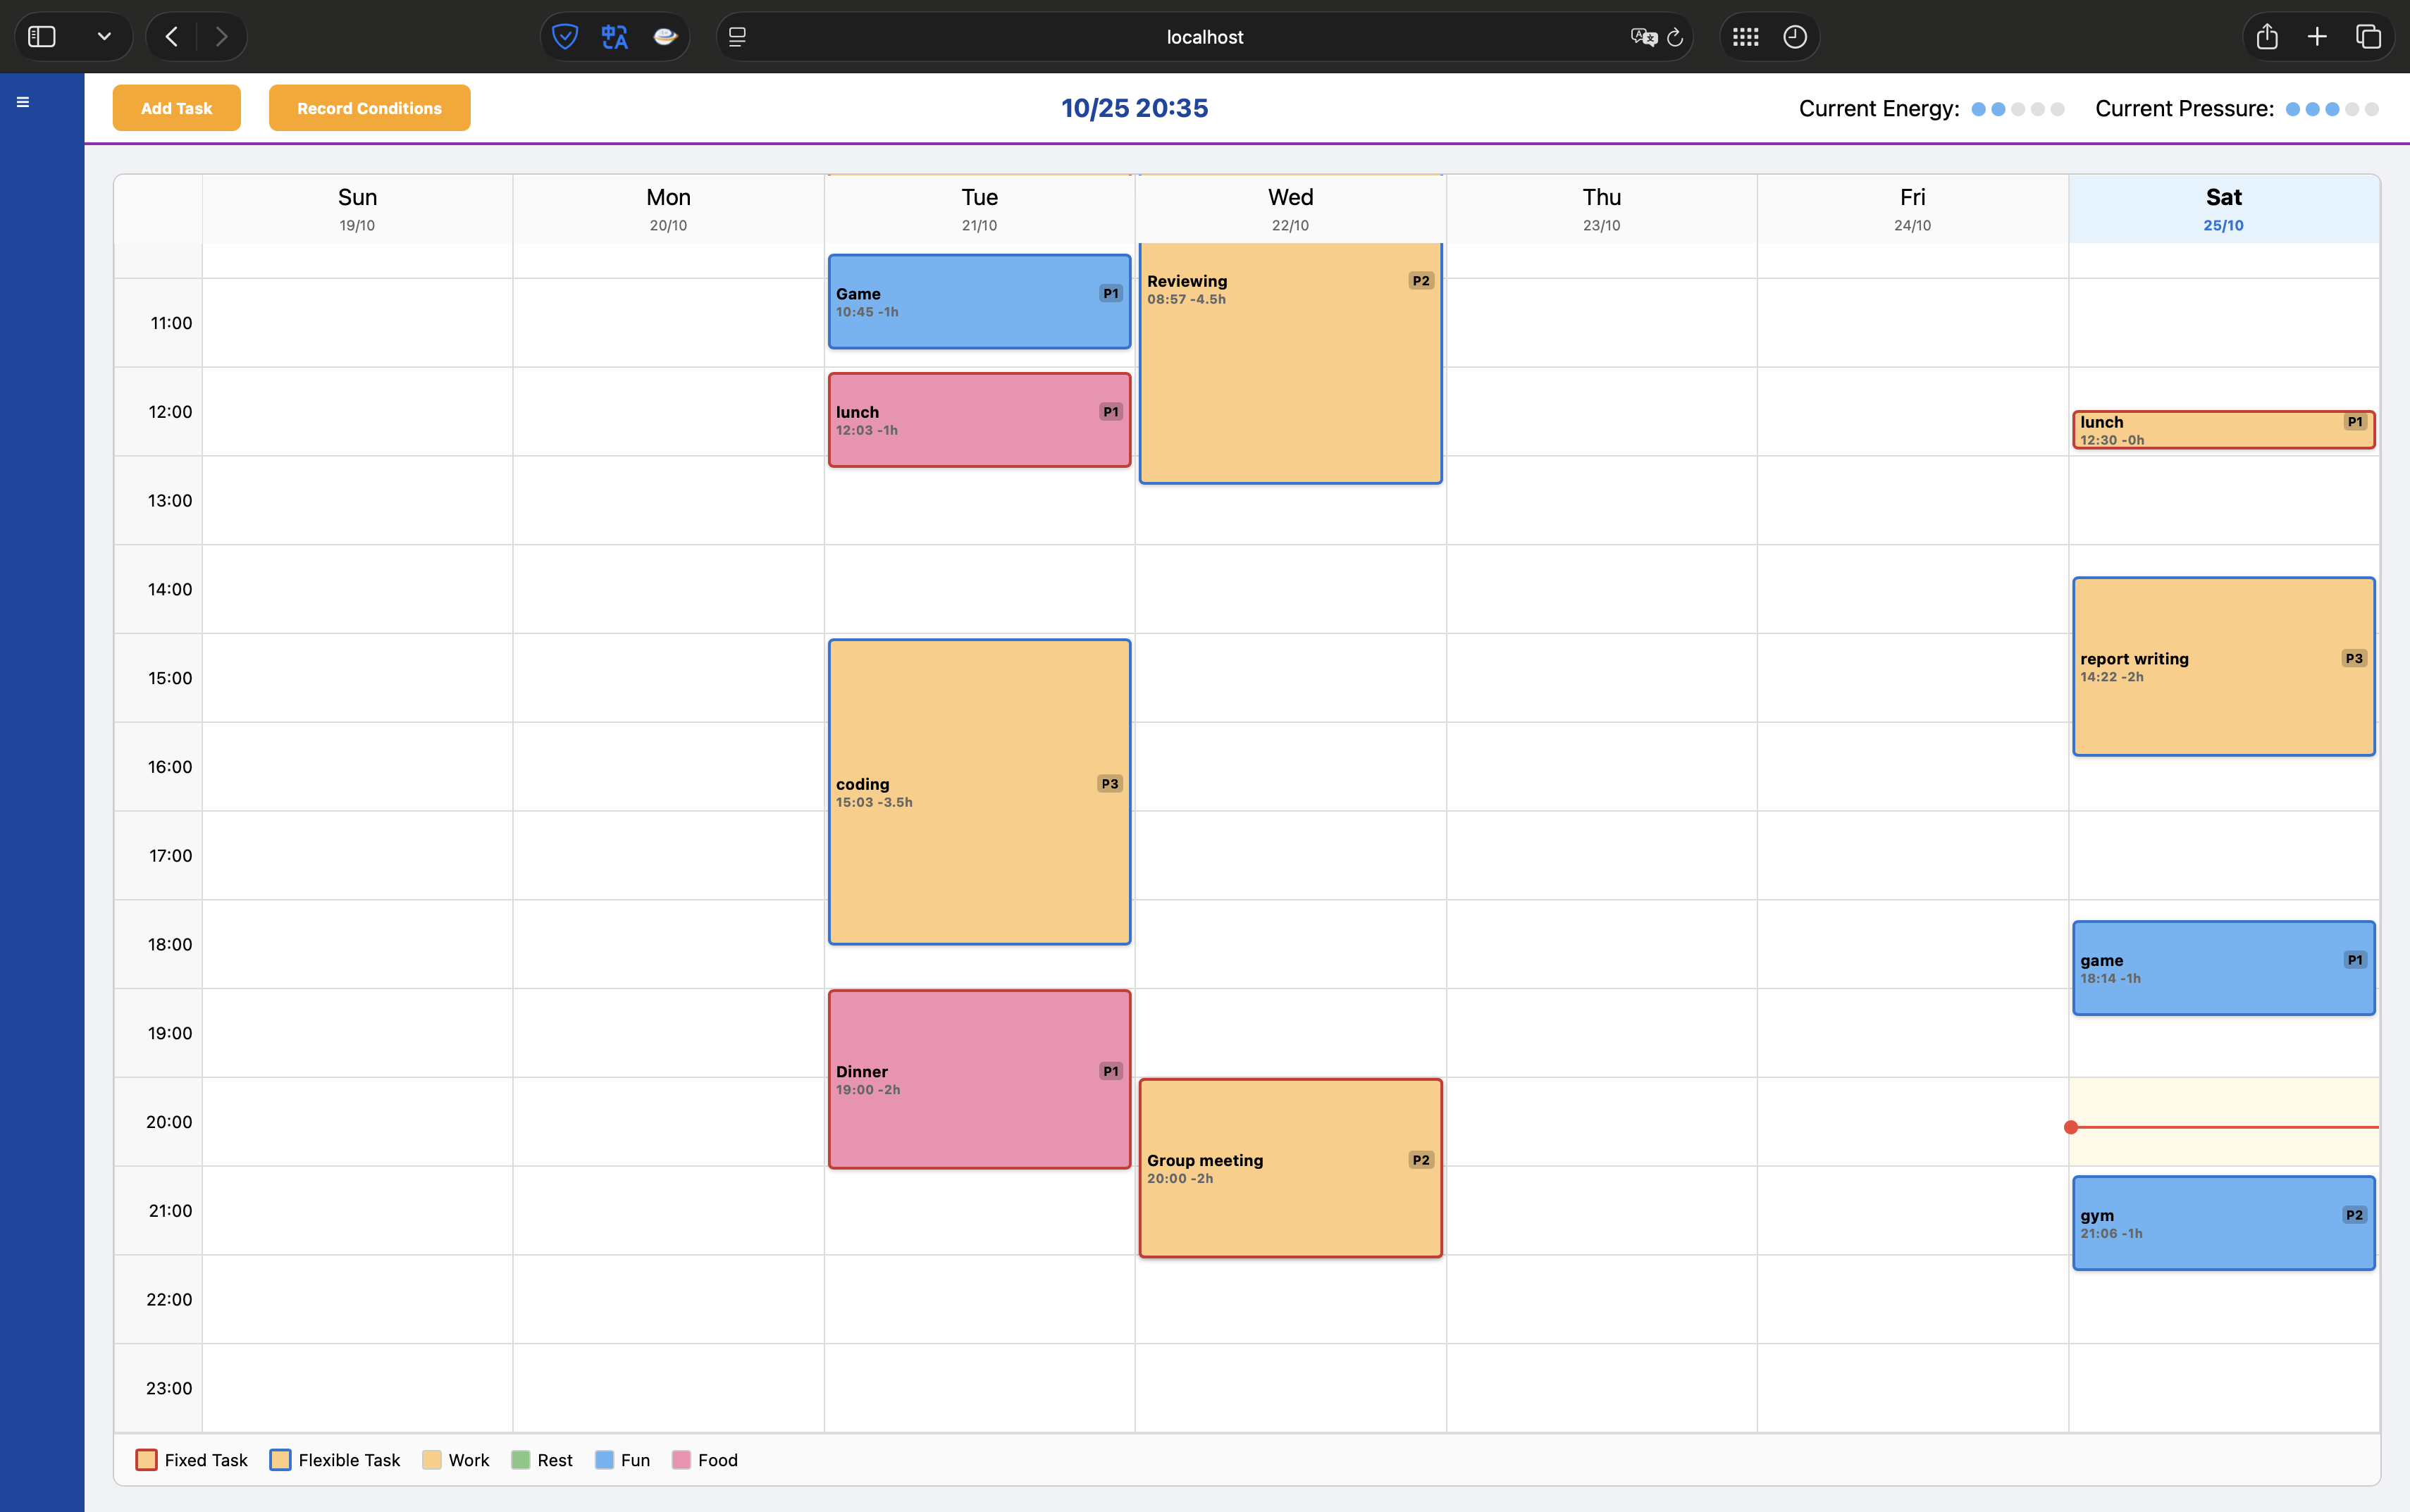
\includegraphics[width=\textwidth]{Images/System/chatbot/bf_ai.png}
                                    \caption{Before AI Assignment}
                                    \label{bf_ai}
                                \end{minipage}
                                \hfill
                                \begin{minipage}[t]{0.49\textwidth}
                                    \centering
                                    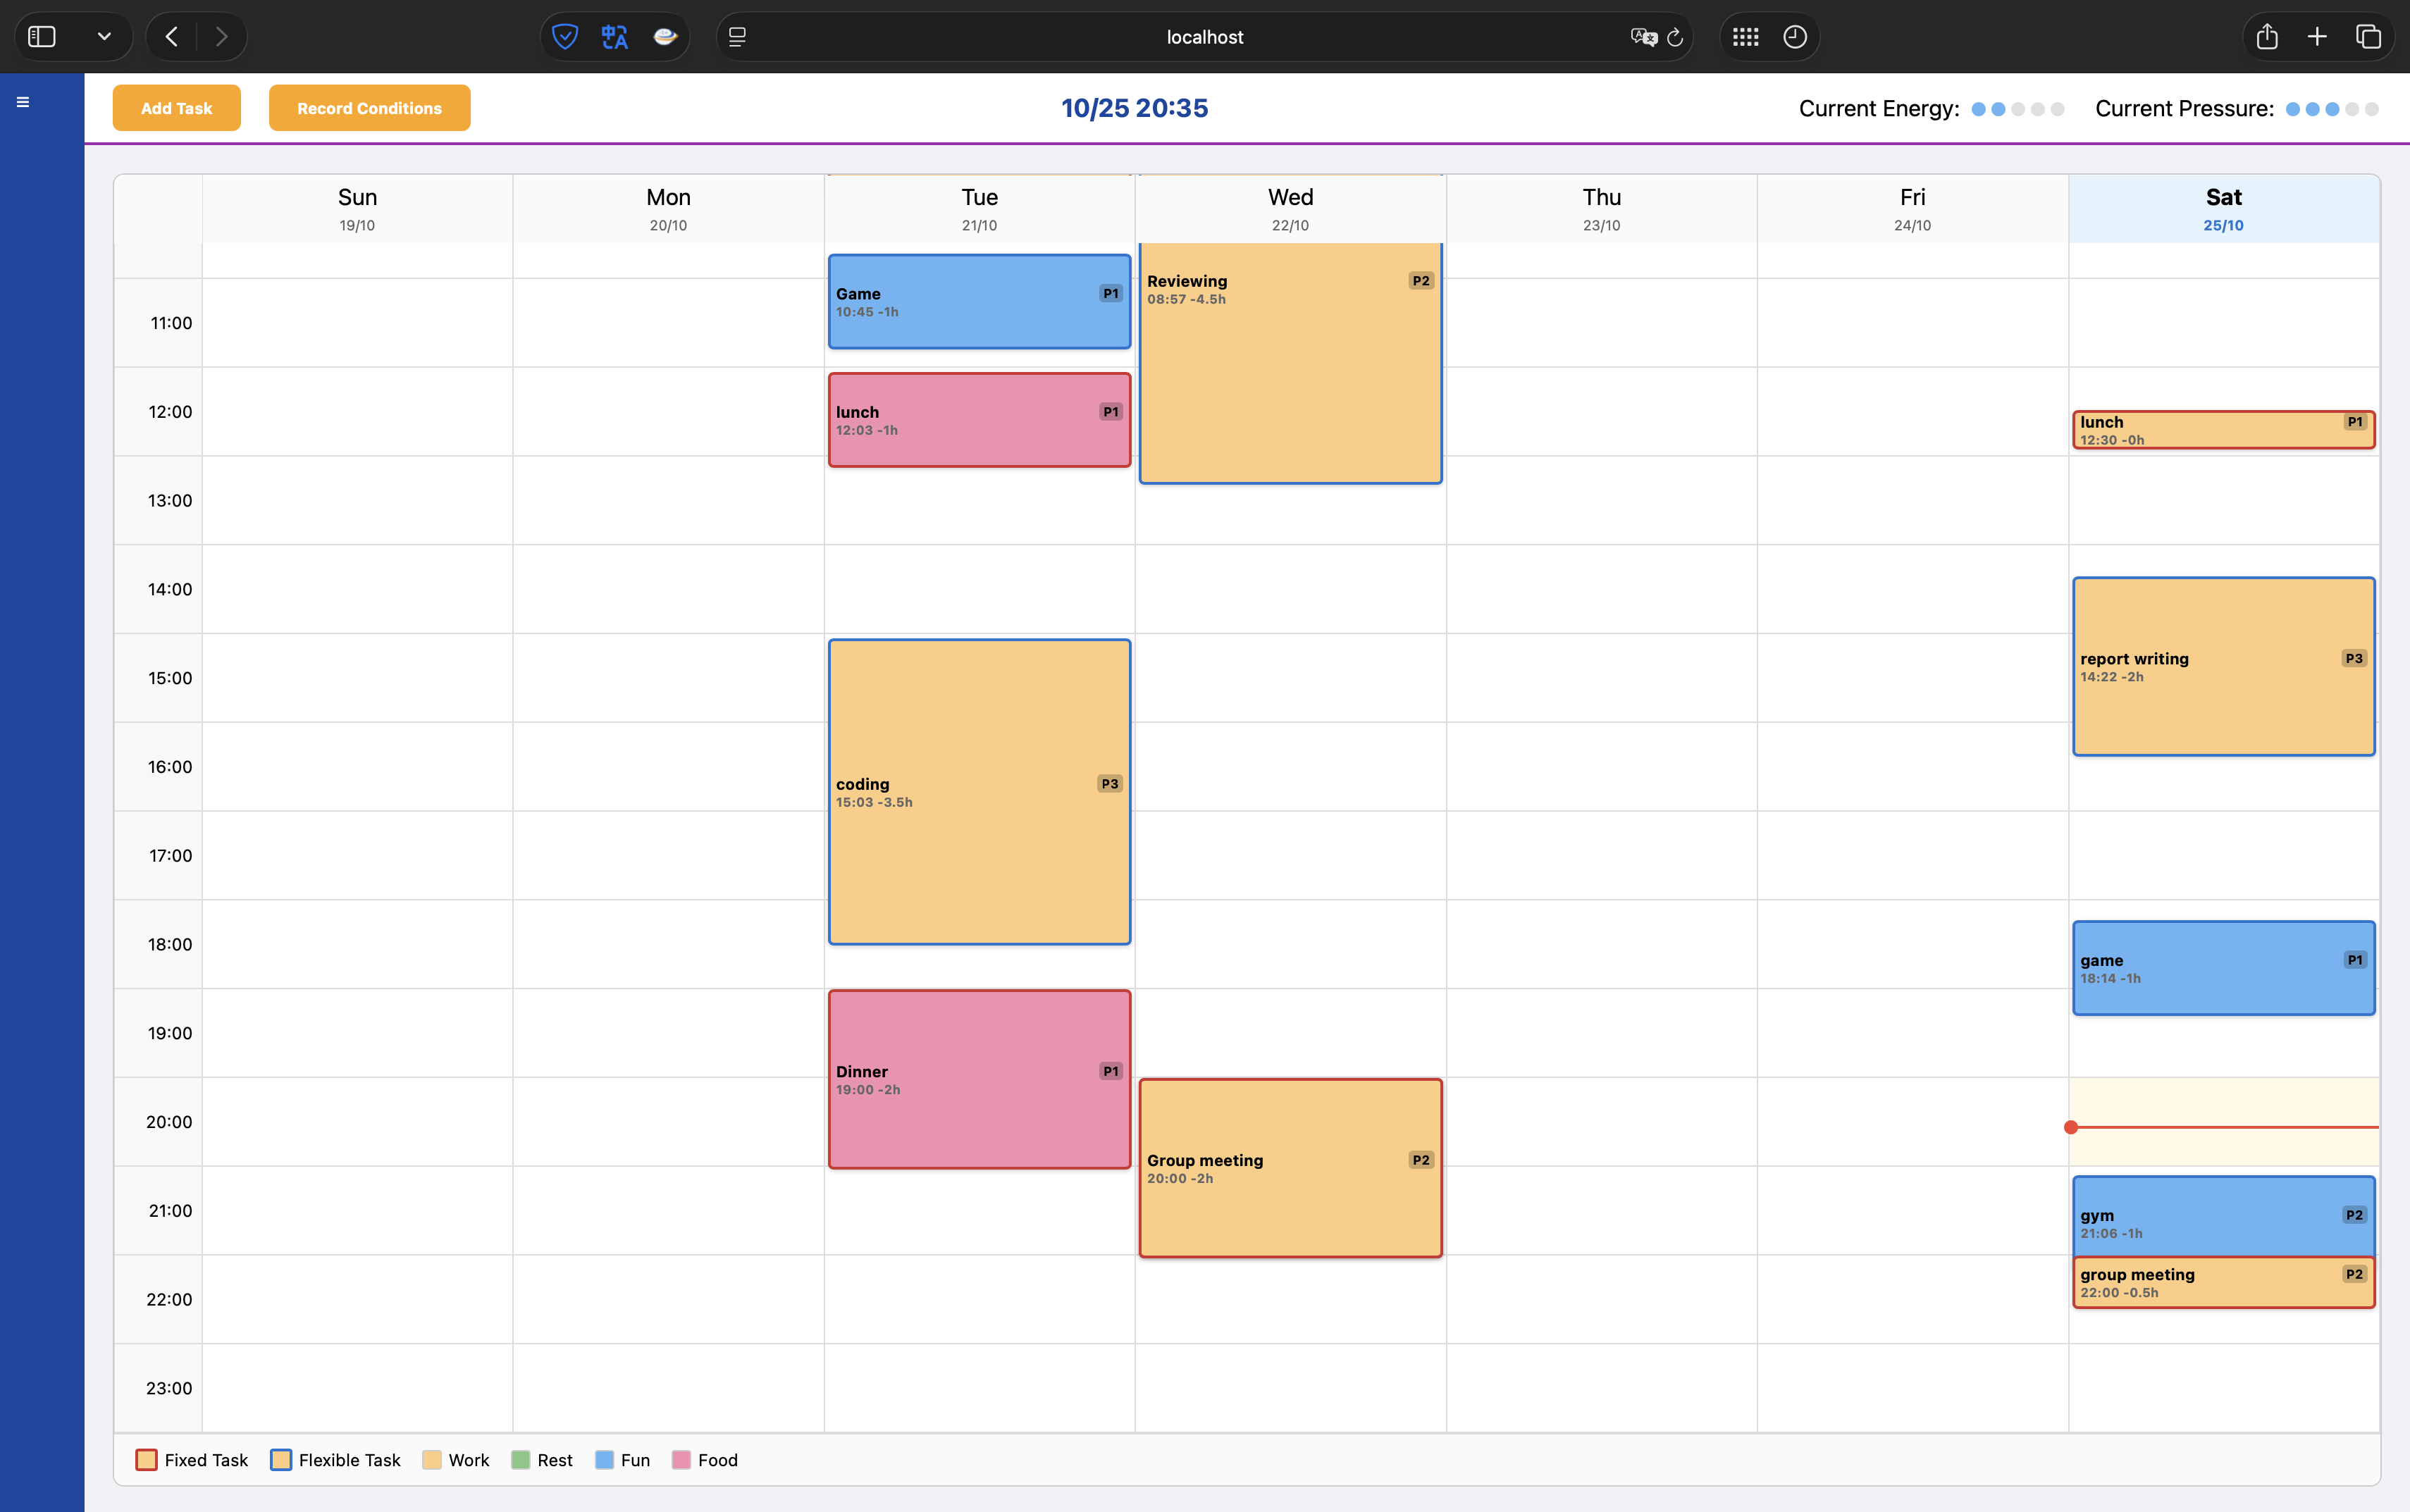
\includegraphics[width=\textwidth]{Images/System/chatbot/aft_ai.png}
                                    \caption{After AI Assignment}
                                    \label{aft_ai}
                                \end{minipage}
                            \end{figure}

                        \item \textbf{Task Creation and Confirmation}  
                
                            Once the LLM successfully interprets the natural language input, the chatbot generates a structured task object and communicates with the backend API to store it in the MongoDB database. A confirmation message is then returned to the user, listing all parsed parameters (name, duration, time, difficulty, priority) for verification. This allows transparent interaction between users and the system, ensuring accuracy and trust in automated scheduling.
                        
                        \item \textbf{Integration with Scheduler}  
                        
                            After task creation, the system instantly synchronizes with the intelligent scheduling engine.  
                            Figure~\ref{bf_ai} and Figure~\ref{aft_ai} illustrate the dynamic scheduling process: the left figure shows the timetable \textbf{before} adding the new task, while the right one shows the \textbf{updated schedule after} the chatbot’s AI-driven assignment.  
                            The scheduler automatically re-evaluates available windows and integrates the new task into an optimized time slot—without requiring manual refresh or adjustment.
                        
                        \item \textbf{User Experience and Significance}  
                        
                            This conversational interface demonstrates how modern large language models can enhance usability and accessibility in AI-driven scheduling systems. It lowers cognitive barriers for non-technical users and allows fluid, human-like communication with the system. Beyond convenience, it embodies the project’s core philosophy — integrating intelligent reasoning with empathetic human-AI interaction.
                            
                    \end{itemize}
                
            \end{enumerate}



%-----------------------
% Conclusion & References
%-----------------------
\section{Conclusion \& References}

In conclusion, the \textbf{AI-Powered Scheduling System} successfully demonstrates how intelligent reasoning and data-driven modeling can be applied to real-world time management. By integrating a neural network–based Task Evaluation Model and a rule-based Scheduler, the system dynamically adapts to users’ changing priorities, energy levels, and workloads. It goes beyond traditional calendar tools by offering personalized recommendations, optimized rest-time allocation, and adaptive rescheduling in response to unexpected events.

Through this project, we illustrate the potential of combining \textbf{artificial intelligence} and \textbf{human-centered design} to improve productivity and well-being simultaneously. The system not only enhances users’ ability to plan and execute daily tasks efficiently but also encourages sustainable work habits that prevent burnout. Although challenges such as limited data availability and user subjectivity remain, the framework establishes a solid foundation for future extensions—such as collaborative scheduling, richer behavioral analytics, and integration with wearable or productivity-tracking devices.

Overall, this work contributes both practically and academically to the development of intelligent personal assistants, marking a step toward more adaptive, context-aware, and empathetic AI systems in everyday life.


\end{document}
%-----------------------
% End document
%-----------------------